\documentclass[oneside]{scrbook}

% Graphics
\usepackage{tikz}
\usepackage{graphicx}
% Maths
\usepackage{amsmath}
\usepackage{amsfonts}
\usepackage{amsthm}
\usepackage{mathtools}
\usepackage{bm}
% Algorithms
\usepackage{algorithmicx}
\usepackage{algpseudocode}
% Local
\usepackage{local_macros/isasmathmacros}

% Environments
\theoremstyle{definition}
\newtheorem{definition}{Definition}[section]

\theoremstyle{definition}
\newtheorem{theorem}{Theorem}[section]

\theoremstyle{remark}
\newtheorem*{remark}{Remark}

% Algorithm settings
\algnewcommand{\LineComment}[1]{\State \(\triangleright\) #1}

% Tikz settings
\usetikzlibrary{math}

% Tikz reused commands
\tikzset{
   plane/.pic = {
    \draw[fill]  plot[smooth, tension=0.6] coordinates {
        (-0.65,-0.9) 
        (-0.6,-0.85) 
        (-0.4,-0.75) 
        (-0.25,-0.65) 
        (-0.15,-0.5) 
        (-0.12,-0.3) 
        (-0.1,-0.1) 
        (0,0) 
        (0.1,-0.1) 
        (0.12,-0.3) 
        (0.15,-0.5) 
        (0.25,-0.65) 
        (0.4,-0.75) 
        (0.6,-0.85) 
        (0.65,-0.9)
        } -- plot[smooth, tension=0.6] coordinates {
        (0.65,-0.9) 
        (0.15,-0.91)
        (0.35,-1.1) 
        (0.37,-1.15)
        } -- plot[smooth, tension=0.6] coordinates {
        (0.37,-1.15)
        (0,-1.12) 
        (-0.37,-1.15) 
        } -- plot[smooth, tension=0.6] coordinates {
        (-0.37,-1.15)
        (-0.35,-1.1) 
        (-0.15,-0.91) 
        (-0.65,-0.9) 
        } -- cycle;
   }
}
\definecolor{pyplotblue}{RGB}{31,119,180}
\definecolor{pyplotorange}{RGB}{255,127,14}
\definecolor{pyplotgreen}{RGB}{44,160,44}



% 
% 8888888888 8888888b.   .d88888b.  888b    888 88888888888 
% 888        888   Y88b d88P" "Y88b 8888b   888     888     
% 888        888    888 888     888 88888b  888     888     
% 8888888    888   d88P 888     888 888Y88b 888     888     
% 888        8888888P"  888     888 888 Y88b888     888     
% 888        888 T88b   888     888 888  Y88888     888     
% 888        888  T88b  Y88b. .d88P 888   Y8888     888     
% 888        888   T88b  "Y88888P"  888    Y888     888     
%                                                           
%                                                           
%                                                           
% 
\title{Data Confidentiality for Distributed Sensor Fusion}
\author{Marko Ristic}
\date{\today}
\titlehead{Dissertation for the Faculty of Computer Science (FIN),\\Otto von Guericke University (OVGU), Magdeburg}
\publishers{{\large Reviewers:}\\\vspace{\baselineskip}Prof. Dr.-Ing. Benjamin Noack (OVGU, Magdeburg, Germany)\\\dots}

\begin{document}
\maketitle

\frontmatter
\tableofcontents

% 
%        d8888  .d8888b.  888    d8P  
%       d88888 d88P  Y88b 888   d8P   
%      d88P888 888    888 888  d8P    
%     d88P 888 888        888d88K     
%    d88P  888 888        8888888b    
%   d88P   888 888    888 888  Y88b   
%  d8888888888 Y88b  d88P 888   Y88b  
% d88P     888  "Y8888P"  888    Y88b 
%                                     
%                                     
%                                     
% 
\chapter{Acknowledgements}
Acks go here.

% 
%        d8888 888888b.    .d8888b.       8888888888 888b    888 
%       d88888 888  "88b  d88P  Y88b      888        8888b   888 
%      d88P888 888  .88P  Y88b.           888        88888b  888 
%     d88P 888 8888888K.   "Y888b.        8888888    888Y88b 888 
%    d88P  888 888  "Y88b     "Y88b.      888        888 Y88b888 
%   d88P   888 888    888       "888      888        888  Y88888 
%  d8888888888 888   d88P Y88b  d88P      888        888   Y8888 
% d88P     888 8888888P"   "Y8888P"       8888888888 888    Y888 
%                                                                
%                                                                
%                                                                
% 
\chapter{Abstract}
Distributed sensing and fusion algorithms are increasingly present in public computing networks and have led to a natural concern for data security in these environments. This thesis aims to present generalisable data fusion algorithms that simultaneously provide strict cryptographic guarantees on user data confidentiality. While fusion algorithms providing some degrees of security guarantees exist, these are typically either provided at the cost of solution generality or lack formal security proofs. Here, novel cryptographic constructs and state-of-the-art encryption schemes are used to develop formal security guarantees for new and generalised data fusion algorithms. Industry standard Kalman filter derivates are modified and existing schemes abstracted such that novel cryptographic notions capturing the required communications can be formalised, while simulations provide an anlysis of practicality. Due to the generality of the presented solutions, broad applications are supported, including autonomous vehicle communications, smart sensor networks and distributed localisation.

% 
%        d8888 888888b.    .d8888b.       8888888b.  8888888888 
%       d88888 888  "88b  d88P  Y88b      888  "Y88b 888        
%      d88P888 888  .88P  Y88b.           888    888 888        
%     d88P 888 8888888K.   "Y888b.        888    888 8888888    
%    d88P  888 888  "Y88b     "Y88b.      888    888 888        
%   d88P   888 888    888       "888      888    888 888        
%  d8888888888 888   d88P Y88b  d88P      888  .d88P 888        
% d88P     888 8888888P"   "Y8888P"       8888888P"  8888888888 
%                                                               
%                                                               
%                                                               
% 
\chapter{Kurzfassung}
German abs goes here.

% 
% 888b    888  .d88888b. 88888888888     d8888 88888888888 8888888 .d88888b.  888b    888 
% 8888b   888 d88P" "Y88b    888        d88888     888       888  d88P" "Y88b 8888b   888 
% 88888b  888 888     888    888       d88P888     888       888  888     888 88888b  888 
% 888Y88b 888 888     888    888      d88P 888     888       888  888     888 888Y88b 888 
% 888 Y88b888 888     888    888     d88P  888     888       888  888     888 888 Y88b888 
% 888  Y88888 888     888    888    d88P   888     888       888  888     888 888  Y88888 
% 888   Y8888 Y88b. .d88P    888   d8888888888     888       888  Y88b. .d88P 888   Y8888 
% 888    Y888  "Y88888P"     888  d88P     888     888     8888888 "Y88888P"  888    Y888 
%                                                                                         
%                                                                                         
%                                                                                         
% 
\chapter{Notation}
Complete notation here.

% 
% 888888b.    .d88888b.  8888888b. Y88b   d88P 
% 888  "88b  d88P" "Y88b 888  "Y88b Y88b d88P  
% 888  .88P  888     888 888    888  Y88o88P   
% 8888888K.  888     888 888    888   Y888P    
% 888  "Y88b 888     888 888    888    888     
% 888    888 888     888 888    888    888     
% 888   d88P Y88b. .d88P 888  .d88P    888     
% 8888888P"   "Y88888P"  8888888P"     888     
%                                              
%                                              
%                                              
% 
\mainmatter

\chapter{Introduction}\label{ch:intro}
Sensor data processing, state estimation and data fusion have long been active areas of research and continue to find applications in modern systems \cite{andersonOptimalFiltering1979,simonOptimalStateEstimation2006}. As distributed networks have become more prevalent over the years, greater stress has been put on the need for broadly applicable algorithms that support varying types of measurements, estimate accuracies and communication availabilities \cite{mutambaraDecentralizedEstimationControl1998,ligginsDistributedDataFusion2012}, finding uses in localisation, weather forecasting, mapping, cooperative computing and more \cite{galanisApplicationsKalmanFilters2006,gillijnsWhatEnsembleKalman2006,geziciLocalizationUltraWidebandRadios2005,sieblerLocalizationMagneticField2020,kiaCooperativeLocalizationMobile2016,sridharCooperativePerceptionAutonomous2019,aulinasSLAMProblemSurvey2008}. In particular, handling cross-correlations between distributed data, especially when they are not known in advance, has been a well-studied difficulty in distributed estimation and is closely tied to the challenges in the field \cite{julierNondivergentEstimationAlgorithm1997,grimeDataFusionDecentralized1994,noackTreatmentDependentInformation2017,radtkeReconstructionCrossCorrelationsConstant2018}. The use of Bayesian estimation methods such as the popular Kalman filter and its non-linear derivatives have become especially prevalent in these applications due to their recursive, often optimal, properties and their suitability for modelling these cross-correlations \cite{chongFortyYearsDistributed2017,haugBayesianEstimationTracking2012,willnerKalmanFilterAlgorithms1976,pfaffInformationFormDistributed2017}. In recent years, widespread advancements in distributed algorithms and the ubiquity of public networks such as the Internet, wireless communication channels and the Internet-of-things (IoT) paradigm, have brought privacy challenges into focus as well \cite{brennerSecretProgramExecution2011,renSecurityChallengesPublic2012}. In particular, the data confidentiality component of the cryptographic Confidentiality-Integrity-Availability (CIA) triad \cite{keyserSecurityPolicy2005} has become an important goal in security-aware distributed data processing tasks. That is for concrete data, private to participants, to remain confidential or leakage to be formally quantifiable. In general, the broader topic of data \textit{privacy}, concerned with the identification of individuals by any means including the observation of this data, is used synonymously in literature \cite{farokhiPrivacyDynamicalSystems2020,specialePrivacyPreservingImageBased2019,erkinPrivacyPreservingFaceRecognition2009,hePreservingDataPrivacyAdded2018,liPrivacyPreservingDistributedOptimization2020} but will not be considered in its entirety in this thesis.

Traditional data confidentiality involves keeping transmitted information private from unauthorised parties in untrusted networks and can often be achieved irrespective of the data processing algorithms used. Typically, these scenarios can be achieved by using common symmetric and asymmetric encryption schemes such as the Advanced Encryption Standard (AES) \cite{gueronIntelAdvancedEncryption2010} or the Rivest-Shamir-Adleman (RSA) cryptosystem \cite{rivestMethodObtainingDigital1978}, respectively. These scenarios, however, imply trust between encrypting and decrypting parties, which cannot always be assumed in distributed environments. Situations where partial results are considered private, or only partial leakage of data is desired for computing results, do not assume this trust and have led to the development of several encryption schemes that provide encrypted operations and explicit formal leakages \cite{paillierPublicKeyCryptosystemsBased1999,shiPrivacyPreservingAggregationTimeSeries2011,chotardDecentralizedMultiClientFunctional2018,andresGeoIndistinguishabilityDifferentialPrivacy2013}. A very applicable group of these schemes in estimation, homomorphic encryption (HE), allow operations to be performed on encrypted data without decryption. These schemes can be loosely grouped into two categories: fully homomorphic encryption (FHE), allowing arbitrary operations on encryptions; and partially homomorphic encryption (PHE), allowing only a subset, typically one, operations. Although FHE suits a wider variety of estimation problems, essentially allowing arbitrary computations while preserving data confidentiality, its current implementations are still too computationally expensive for large-scale or real-time processing \cite{acarSurveyHomomorphicEncryption2018,gentryFullyHomomorphicEncryption2009,stehleFasterFullyHomomorphic2010}. For this reason, PHE has been the more popular choice in providing data confidentiality during a variety of estimation tasks \cite{lagendijkEncryptedSignalProcessing2012,ryanPretVoterPaillier2008,kerschbaumOutsourcedPrivateSet2012,catalanoUsingLinearlyHomomorphicEncryption2015,abdallaSingleInputMulticlientInnerProduct2019} and is predominantly relied on throughout this thesis. While these schemes provide a powerful tool for designing data-processing algorithms, the nature of cryptographic analysis in distributed environments depends heavily on communication protocols between participants, limiting the ease of their combination with general estimation and data fusion solutions such as the Bayesian methods mentioned previously. In turn, this has led to various context-specific estimation solutions with differing degrees of cryptographic guarantees, often restricting general solutions to provide meaningful cryptographic guarantees or foregoing provable security for more general algorithms. This leads us to the goals of this thesis and the current state-of-the-art in security-oriented estimation and data fusion.

% 
%  .d8888b.   .d88888b. 88888888888     d8888 
% d88P  Y88b d88P" "Y88b    888        d88888 
% Y88b.      888     888    888       d88P888 
%  "Y888b.   888     888    888      d88P 888 
%     "Y88b. 888     888    888     d88P  888 
%       "888 888     888    888    d88P   888 
% Y88b  d88P Y88b. .d88P    888   d8888888888 
%  "Y8888P"   "Y88888P"     888  d88P     888 
%                                             
%                                             
%                                             
% 

\section{Research Questions and the State-of-the-Art}\label{sec:intro:sota}
The restrictions on the generality of solutions and the frequent foregoing of cryptographic guarantees when providing security in estimation tasks form the literature gap that this thesis is centred around. The overarching topics we are interested in are as follows. We wish to find distributed estimation and data fusion solutions based on the Kalman filter for non-linear models with provable security. Here, non-linear models capture the broadest, and therefore most generally applicable, solutions in estimation. Secondly, we are interested in formalising novel cryptographic definitions that capture suitable communication protocols and leakages for any of these solutions should they not exist. Lastly, we would like to define a general cryptographic notion that captures adversary estimation performance and can be applied to existing security-aware estimation schemes with no cryptographically provable guarantees. From these topics, we concentrate on three specific problems that will form the main chapters of this thesis and discuss the state-of-the-art in the context of each.

% 
% ######## ##     ##  ######  ####  #######  ##    ## 
% ##       ##     ## ##    ##  ##  ##     ## ###   ## 
% ##       ##     ## ##        ##  ##     ## ####  ## 
% ######   ##     ##  ######   ##  ##     ## ## ## ## 
% ##       ##     ##       ##  ##  ##     ## ##  #### 
% ##       ##     ## ##    ##  ##  ##     ## ##   ### 
% ##        #######   ######  ####  #######  ##    ## 
% 

\subsection{Estimate Fusion on an Untrusted Cloud}\label{subsec:intro:conf_est_fusion}
The first problem we consider is confidential estimate fusion on a centralised untrusted cloud. This is a popular scenario in distributed sensor fusion, where a cloud or fusing party obtains estimates from within the network and fuses them centrally, providing a resulting fused state estimate for further processing []. Some use cases for the scenario include factory sensor data fusion, object tracking, centralised weather forecasting, etc. Intuitively, untrusted cloud processing brings security concerns to mind, such as the confidentiality of individual estimate data and the privacy of participants producing it []. Work on security-aware cloud processing and data fusion exists in a variety of scenarios []. FHE and PHE are particularly suited to the problem, allowing computations to be finalised on confidential data before being queried by trusted parties for final results []. This includes control aggregation [], private matrix multiplication [] and private set intersection []. Another relevant topic is differential privacy []. Here, a formal cryptographic notion guarantees that individual inputs to data fusion cannot be exactly estimated by guaranteeing that results are indistinguishable when differing by only a single input. The downside to this cryptographically meaningful and often applicable solution is the noisiness of fusion results, rendering it unsuitable for scenarios where result accuracy cannot be compromised. We are interested in accurate general solutions to data fusion in a Bayesian setting and our solution to this problem aims to fuse arbitrary (non-linear and dependent) state estimates accurately while a strong cryptographically meaningful assessment of the level of confidentiality can be provided. Some applicable methods for this exist, albeit restricting the estimation or security requirements. In [darup two clouds], control inputs can be computed in an encrypted control loop, with methods applicable to estimation, but rely on the presence of two clouds that cannot maliciously collude. [aristov] presents a method for homomorphic fusion but requires that partial fusions are collected in a hierarchical network and for fused measurements to be linear and independent. While in [proloc], the homomorphic fusion of data is used to perform range-measurement localisation on confidential measurements but does not lend itself to a Bayesian setting where measurement noise properties are considered. The formalised estimation problem and cryptographic goals as well as our novel solutions to this problem are presented in chapter \ref{ch:cloud_fusion}.

% 
% ##    ##  #######  ##    ## ##       #### ##    ## 
% ###   ## ##     ## ###   ## ##        ##  ###   ## 
% ####  ## ##     ## ####  ## ##        ##  ####  ## 
% ## ## ## ##     ## ## ## ## ##        ##  ## ## ## 
% ##  #### ##     ## ##  #### ##        ##  ##  #### 
% ##   ### ##     ## ##   ### ##        ##  ##   ### 
% ##    ##  #######  ##    ## ######## #### ##    ## 
% 

\subsection{Distributed Non-Linear Measurement Fusion with Untrusted Participants}\label{subsec:intro:conf_nonlin_measurements}
The next problem we look at is confidential measurement fusion when participants in the network are untrusted. The scenario is in principle similar to the fusion problem in section \ref{subsec:intro:conf_est_fusion} but is distinguished by the party using the fusion result and the properties of the measurements. Unlike using a cloud, final computed fusion results are often needed by the party computing the fusion itself [], such as self-localisation and decentralised estimation [], rendering HE methods less practical as no trusted querying party is present. We also distinguish measurements from estimates in that we assume they are independent, allowing for the use of accurate Bayesian estimation methods such as the Kalman filter which make this assumption []. Methods [aristov] and [proloc] again tackle a similar problem, but remain limited in requiring a hierarchical communication network and not considering measurement noise properties. Similarly to the fusion problem above, differential privacy [] is again a related and applicable field, including existing applications to the Kalman filter [], but results remain noisy and are considered undesirable when accuracy is important. To provide an accurate non-linear distributed estimation filter with meaningful cryptographic assessment, other cryptographic notions need to be considered. Cryptographic constructs that support homomorphic computations as well as the leakage of final results, as would be required in the case where a third-party cloud is not used, exist. Private Weighted Sum Aggregation with centralised or hidden weights (pWSAc and pWSAh, respectively) are introduced in [pwsac] and [pwsah in lcao paper] as a means for computing control inputs in a distributed network without leaking individual contributions. Here, formal definitions with different communication assumptions to those suitable in a non-linear estimation problem are given. Similarly, more definitions of aggregation schemes have been introduced [shi, joyelibert, joyelibert extension, data aggregation scheme secret sharing] with a variety of specified communication protocols. Again, a formalised estimation and cryptographic goal for this problem as well as the presented solutions will be shown in chapter \ref{ch:nonlin_fusion}.

% 
% ########  ######## ########  ######## 
% ##     ## ##       ##     ## ##       
% ##     ## ##       ##     ## ##       
% ########  ######   ########  ######   
% ##        ##       ##   ##   ##       
% ##        ##       ##    ##  ##       
% ##        ######## ##     ## ##       
% 

\subsection{Provable Estimate Performances}\label{subsec:intro:provable_est_perf}

eavesdropper paper with a secure return channel and a lossier channel for eavesdroppers

GPS

chaotic system paper

physical layer noise paper (similar to chaotic noise paper)

data privacy with added noises paper (semantic security where we consider computational)


--

privacy-preserving image-based localisation??


This problem, it's cryptographic goals and presented solutions are formalised in chapter \ref{ch:priv_estimation}.

% 
%  .d8888b.   .d88888b.  888b    888 88888888888 
% d88P  Y88b d88P" "Y88b 8888b   888     888     
% 888    888 888     888 88888b  888     888     
% 888        888     888 888Y88b 888     888     
% 888        888     888 888 Y88b888     888     
% 888    888 888     888 888  Y88888     888     
% Y88b  d88P Y88b. .d88P 888   Y8888     888     
%  "Y8888P"   "Y88888P"  888    Y888     888     
%                                                
%                                                
%                                                
% 

\section{Contributions}\label{sec:intro:contributions}

The contributions tackle the research topics in section .. by considering three concrete problems that coincide with the broader problems in the field

\begin{itemize}
    \item dot point topics
\end{itemize}



% 
%  .d8888b. 88888888888 8888888b.  888     888  .d8888b. 88888888888 
% d88P  Y88b    888     888   Y88b 888     888 d88P  Y88b    888     
% Y88b.         888     888    888 888     888 888    888    888     
%  "Y888b.      888     888   d88P 888     888 888           888     
%     "Y88b.    888     8888888P"  888     888 888           888     
%       "888    888     888 T88b   888     888 888    888    888     
% Y88b  d88P    888     888  T88b  Y88b. .d88P Y88b  d88P    888     
%  "Y8888P"     888     888   T88b  "Y88888P"   "Y8888P"     888     
%                                                                    
%                                                                    
%                                                                    
% 

\section{Thesis Structure}\label{sec:intro:structure}

Each chapter includes a formal problem formalisation before presenting the novel solutions.

\chapter{Preliminaries}\label{ch:prelims}
When introducing novel methods throughout this thesis, we make use of several existing algorithms and constructs. In this chapter, we present these relevant preliminaries grouped by the fields they pertain to; estimation and cryptography.

% 
% 8888888888 .d8888b. 88888888888      8888888b.  8888888b.  8888888888 888      8888888 888b     d888 
% 888       d88P  Y88b    888          888   Y88b 888   Y88b 888        888        888   8888b   d8888 
% 888       Y88b.         888          888    888 888    888 888        888        888   88888b.d88888 
% 8888888    "Y888b.      888          888   d88P 888   d88P 8888888    888        888   888Y88888P888 
% 888           "Y88b.    888          8888888P"  8888888P"  888        888        888   888 Y888P 888 
% 888             "888    888          888        888 T88b   888        888        888   888  Y8P  888 
% 888       Y88b  d88P    888          888        888  T88b  888        888        888   888   "   888 
% 8888888888 "Y8888P"     888          888        888   T88b 8888888888 88888888 8888888 888       888 
%                                                                                                      
%                                                                                                      
%                                                                                                      
% 

\section{Estimation Preliminaries}\label{sec:prelims:est_prelims}
Sensor and estimate data that we consider is primarily Bayesian in nature and typically consists of estimates and associated estimate uncertainties. The linear Kalman filter and the linearising extended Kalman filter, along with their information filter equivalents, are particularly useful in the estimation and fusion of such data. A general fusion algorithm, the covariance intersection, used when data cross-correlations are unknown, is also introduced.

% 
% ##    ## ######## 
% ##   ##  ##       
% ##  ##   ##       
% #####    ######   
% ##  ##   ##       
% ##   ##  ##       
% ##    ## ##       
% 

\subsection{Kalman Filter}\label{subsec:prelims:kf}
The Kalman filter (KF) [orig kf] is a popular and well studied recursive state estimation filter that produces estimates and their error covariances $\hat{\vec{x}}_{k|k^\prime} \in \mathbb{R}^n$ and $\mat{P}_{k|k^\prime} \in \mathbb{R}^{n \times n}$, respectively, for a timestep $k \in \mathbb{N}$, given measurements up to and including timestep $k^\prime \in \mathbb{N}$ [kf uses]. Although the KF supports the estimation of a system state which can be manipulated through an external input, this thesis primarily discusses scenarios where no external inputs are known to the estimator and will introduce the filter with these inputs set to $\vec{0}$. In this form, the KF assumes the existence of a true state $\vec{x}_k \in \mathbb{R}^n$ at each timestep $k$, following the linear process model
\begin{equation}\label{eq:prelims:lin_gauss_process_model}
    \vec{x}_k = \mat{F}_k \vec{x}_{k-1} + \vec{w}_k\,,
\end{equation}
where $\vec{w}_k \sim \mathcal{N}(\vec{0}, \mat{Q}_k)$ with known covariance $\mat{Q}_k \in \mathbb{R}^{n \times n}$. Similarly, measurements $\vec{z}_k \in \mathbb{R}^m$ are assumed to follow the linear measurement model
\begin{equation}\label{eq:prelims:lin_gauss_measurement_model}
    \vec{z}_k = \mat{H}_k \vec{x}_k + \vec{v}_k\,,
\end{equation}
where $\vec{v}_k \sim \mathcal{N}(\vec{0}, \mat{R}_k)$ with known covariance $\mat{R}_k \in \mathbb{R}^{m \times m}$. The filter requires initialisation with some known values $\hat{\vec{x}}_{0|0}$ and $\mat{P}_{0|0}$ and is computed recursively in two steps. First, the estimate for the next timestep is predicted without new measurement information, known as the \textit{prediction} step, and is given by
\begin{equation}\label{eq:prelims:kf_est_predict}
    \hat{\vec{x}}_{k|k-1} = \mat{F}_k \hat{\vec{x}}_{k-1|k-1}
\end{equation}
and
\begin{equation}\label{eq:prelims:kf_cov_predict}
    \mat{P}_{k|k-1} = \mat{F}_k \mat{P}_{k-1|k-1} \mat{F}_k^\top + \mat{Q}_k\,.
\end{equation}
Next, this prediction is updated with current measurement information, known as the \textit{update} step, and given by
\begin{equation}\label{eq:prelims:kf_est_update}
    \hat{\vec{x}}_{k|k} = \hat{\vec{x}}_{k|k-1}+\mat{P}_{k|k-1}\mat{H}_k^\top\left(\mat{H}_k\mat{P}_{k|k-1}\mat{H}_k^\top + \mat{R}_k\right)^{-1}\left(z_k-\mat{H}_k\hat{\vec{x}}_{k|k-1}\right)
\end{equation}
and
\begin{equation}\label{eq:prelims:kf_cov_update}
    \mat{P}_{k|k} = \mat{P}_{k|k-1}-\mat{P}_{k|k-1}\mat{H}_k^\top\left(\mat{H}_k\mat{P}_{k|k-1}\mat{H}_k^\top + \mat{R}_k\right)^{-1}\mat{H}\mat{P}_{k|k-1}\,.
\end{equation}
In addition to alternating prediction and update steps as time progresses, the update step \eqref{eq:prelims:kf_est_update} and \eqref{eq:prelims:kf_cov_update} can be skipped at timesteps when no measurements are available. Similarly, when multiple independent measurements are present at the same timestep, the update step can be repeated for each measurement individually. Detailed derivations of the KF and discussions on its properties can be found in [huag+chap].

% 
% ##    ## ########     #######  ########  ######## 
% ##   ##  ##          ##     ## ##     ##    ##    
% ##  ##   ##          ##     ## ##     ##    ##    
% #####    ######      ##     ## ########     ##    
% ##  ##   ##          ##     ## ##           ##    
% ##   ##  ##          ##     ## ##           ##    
% ##    ## ##           #######  ##           ##    
% 

\subsection{Kalman Filter Optimality}\label{subsec:prelims:kf_opt}
One of the reasons for the ubiquity and popularity of the KF introduced in section \ref{subsec:prelims:kf} is its optimality in terms of mean square error (MSE) [huag+chap]. That is, the estimate's error covariances, defined by the expectation capturing mean square error,
\begin{equation}
    \mat{P}_{k|k} = \mathbb{E}\left\{\left(\vec{x}_k - \hat{\vec{x}}_{k|k}\right)\left(\vec{x}_k - \hat{\vec{x}}_{k|k}\right)^\top\right\}\,,
\end{equation}
and computed by \eqref{eq:prelims:kf_cov_predict} and \eqref{eq:prelims:kf_cov_update}, can be shown to equal the theoretical lower bound on the covariance of an unbiased estimator when process and measurement models \eqref{eq:prelims:lin_gauss_process_model} and \eqref{eq:prelims:lin_gauss_measurement_model}, respectively, capture the estimated environment exactly [huag refs for crlb]. This property will be used in later cryptographic discussions in this thesis to guarantee estimator performances in terms of MSE. Further reading on the definitions and proofs of KF optimality can be found in [crlb,huag,etc].

% 
% ######## ##    ## ######## 
% ##       ##   ##  ##       
% ##       ##  ##   ##       
% ######   #####    ######   
% ##       ##  ##   ##       
% ##       ##   ##  ##       
% ######## ##    ## ##       
% 

\subsection{Extended Kalman Filter}\label{subsec:prelims:ekf}
The extended Kalman filter (EKF) is a recursive state estimation filter applicable to non-linear models and closely related to the linear KF [ekf paper,huag+chap]. The filter produces estimates and their covariances at each timestep by linearising models at the current estimate and evaluating the filter similarly to the KF. As in the KF, a true state $\vec{x}_k$ is assumed to follow known models. The process model is now non-linear and given by
\begin{equation}\label{eq:prelims:nonlin_gauss_process_model}
    \vec{x}_k = f_k(\vec{x}_{k-1}) + \vec{w}_k\,,
\end{equation}
where again $\vec{w}_k \sim \mathcal{N}(\vec{0}, \mat{Q}_k)$ with known covariance $\mat{Q}_k$. Similarly, measurements are assumed to follow the non-linear measurement model
\begin{equation}\label{eq:prelims:nonlin_gauss_measurement_model}
    \vec{z}_k = h_k(\vec{x}_k) + \vec{v}_k\,,
\end{equation}
with $\vec{v}_k \sim \mathcal{N}(\vec{0}, \mat{R}_k)$ and known covariance $\mat{R}_k$. The EKF \textit{prediction} step is given by
\begin{equation}\label{eq:prelims:ekf_est_predict}
    \hat{\vec{x}}_{k|k-1} = f_k\left(\hat{\vec{x}}_{k-1|k-1}\right)
\end{equation}
and
\begin{equation}\label{eq:prelims:ekf_cov_predict}
    \mat{P}_{k|k-1} = \hat{\mat{F}}_k \mat{P}_{k-1|k-1} \hat{\mat{F}}_k^\top + \mat{Q}_k\,,
\end{equation}
with Jacobian
\begin{equation}\label{eq:prelims:ekf_predict_jacobian}
    \hat{\mat{F}}_k = \left.\frac{\partial f_k}{\partial \vec{x}}\right|_{\hat{\vec{x}}_{k-1|k-1}}
\end{equation}
linearising the process model at the latest estimate for estimate error covariance prediction. The EKF \textit{update} step is given by
\begin{equation}\label{eq:prelims:ekf_est_update}
    \hat{\vec{x}}_{k|k} = \hat{\vec{x}}_{k|k-1}+\mat{P}_{k|k-1}\hat{\mat{H}}_k^\top\left(\hat{\mat{H}}_k\mat{P}_{k|k-1}\hat{\mat{H}}_k^\top + \mat{R}_k\right)^{-1}\left(z_k-h_k(\hat{\vec{x}}_{k|k-1})\right)
\end{equation}
and
\begin{equation}\label{eq:prelims:ekf_cov_update}
    \mat{P}_{k|k} = \mat{P}_{k|k-1}-\mat{P}_{k|k-1}\hat{\mat{H}}_k^\top\left(\hat{\mat{H}}_k\mat{P}_{k|k-1}\hat{\mat{H}}_k^\top + \mat{R}_k\right)^{-1}\hat{\mat{H}}\mat{P}_{k|k-1}\,,
\end{equation}
with Jacobian
\begin{equation}\label{eq:prelims:ekf_update_jacobian}
    \hat{\mat{H}}_k = \left.\frac{\partial h_k}{\partial \vec{x}}\right|_{\hat{\vec{x}}_{k|k-1}}
\end{equation}
linearising the measurement model. Unlike the linear KF, by linearising the models the EKF propagates Gaussian model noises in its estimates that may not be Gaussian in reality, even when process and measurement models \eqref{eq:prelims:nonlin_gauss_process_model} and \eqref{eq:prelims:nonlin_gauss_measurement_model}, respectively, are exactly correct. For this reason, the EKF does not hold the same guarantees on optimality as the KF does. To a similar effect, highly non-linear models or inaccurate models can lead to greater inaccuracies and divergence of estimates from true states in EKF estimates. Despite these downsides, its scalability and efficiency have made the EKF an industry-standard estimation filter for non-linear systems [smth on uses of ekf]. More details on the EKF and its derivation can be found in [huag+chap].

% 
% #### ######## 
%  ##  ##       
%  ##  ##       
%  ##  ######   
%  ##  ##       
%  ##  ##       
% #### ##       
% 

\subsection{Information Filter}\label{subsec:prelims:if}
The information filter (IF) is an algebraic reformulation of the KF from section \ref{subsec:prelims:kf} [niehsenInformationFusionBased2002, Mutambara, another]. The information form of the filter simplifies the update step of the filter making it more suitable when multiple independent measurements are present at the same timestep. The key difference of the IF is the storing and propagation of the information vector $\hat{\vec{y}}_{k|k'}$ and information matrix $\mat{Y}_{k|k'}$ rather than the estimate and its error covariance, $\hat{\vec{x}}_{k|k'}$ and $\mat{P}_{k|k'}$, respectively, stored by the KF. When assuming the same linear and Gaussian models \eqref{eq:prelims:lin_gauss_process_model} and \eqref{eq:prelims:lin_gauss_measurement_model}, the information vector and matrix are related to the estimate and its covariance by
\begin{equation}\label{eq:prelims:info_vec_defn}
    \hat{\vec{y}}_{k|k'} = \mat{P}_{k|k'}^{-1}\hat{\vec{x}}_{k|k'}
\end{equation}
and
\begin{equation}\label{eq:prelims:info_mat_defn}
    \mat{Y}_{k|k'} = \mat{P}_{k|k'}^{-1}\,,
\end{equation}
for an estimated timestep $k$ and measurements from timesteps up to and including $k'$. The estimation of the information vector and information matrix requires an initialisation of $\hat{\vec{y}}_{0|0}$ and $\mat{Y}_{0|0}$, similarly to the KF, and is also performed by iterating distinct predict and update filter steps. The prediction step is given by
\begin{equation}\label{eq:prelims:if_info_vec_predict}
    \hat{\vec{y}}_{k|k-1} = \mat{Y}_{k|k-1}\mat{F}_k\mat{Y}_{k-1|k-1}^{-1}\hat{\vec{y}}_{k-1|k-1}
\end{equation}
and
\begin{equation}\label{eq:prelims:if_info_mat_predict}
    \mat{Y}_{k|k-1} = \left(\mat{F}_k\mat{Y}_{k-1|k-1}^{-1}\mat{F}_k^\top + \mat{Q}_k\right)^{-1}\,.
\end{equation}
The update step is given by
\begin{equation}\label{eq:prelims:if_info_vec_update_single}
    \hat{\vec{y}}_{k|k} = \hat{\vec{y}}_{k|k-1} + \vec{i}_k
\end{equation}
and
\begin{equation}\label{eq:prelims:if_info_mat_update_single}
    \mat{Y}_{k|k} = \mat{Y}_{k|k-1} + \mat{I}_k\,,
\end{equation}
where added terms $\vec{i}_k$ and $\mat{I}_k$ are known as the measurement vector and measurement matrix, respectively, and are defined as
\begin{equation}
    \vec{i}_k = \mat{H}_k^\top\mat{R}_k^{-1}z_k
\end{equation}
and
\begin{equation}
    \mat{I}_k = \mat{H}_k^\top\mat{R}_k^{-1}\mat{H}_k\,.
\end{equation}

Since all information related to a measurement and its sensor are captured in $\vec{i}_k$ and $\mat{I}_k$, namely the measured value $z_k$, measurement model $\mat{H}_k$ and measurement error $\mat{R}_k$, sequential IF update steps required in the presence of multiple sensors are easily computed as a summation of this information from each sensor. That is, if we consider the same process model \eqref{eq:prelims:lin_gauss_process_model} and multiple sensors $i$, $1\leq i\leq n$, making independent measurements that follow models
\begin{equation}
    \vec{z}_{k,i} = \mat{H}_{k,i} \vec{x}_k + \vec{v}_{k,i}\,,
\end{equation}
with $\vec{v}_{k,i}\sim\mathcal{N}(\vec{0},\mat{R}_{k,i})$ and known covariances $\mat{R}_{k,i}$, the update step of the filter using all measurements at timestep $k$ can be written as
\begin{equation}\label{eq:prelims:if_info_vec_update}
    \hat{\vec{y}}_{k|k} = \hat{\vec{y}}_{k|k-1} + \sum_{i=1}^n\vec{i}_{k,i}
\end{equation}
and
\begin{equation}\label{eq:prelims:if_info_mat_update}
    \mat{Y}_{k|k} = \mat{Y}_{k|k-1} + \sum_{i=1}^n\mat{I}_{k,i}\,,
\end{equation}
where information vectors $\vec{i}_{k,i}$ and information matrices $\mat{I}_{k,i}$ are now dependent on sensor $i$ and given by
\begin{equation}\label{eq:prelims:if_measurement_vec_defn}
    \vec{i}_{k,i} = \mat{H}_{k,i}^\top\mat{R}_{k,i}^{-1}z_{k,i}
\end{equation}
and
\begin{equation}\label{eq:prelims:if_measurement_mat_defn}
    \mat{I}_{k,i} = \mat{H}_{k,i}^\top\mat{R}_{k,i}^{-1}\mat{H}_{k,i}\,.
\end{equation}
The easily computed summation has led to the IF being particularly suited to distributed estimation environments, where multiple sensors are present and communicational costs need to be reduced [if egs]. In addition, since the IF is strictly a rearrangement of terms in the KF, it holds the same optimality properties as the KF, described in section \ref{subsec:prelims:kf_opt}. For additional reading on the IF, see [mutambara+chap].

% 
% ######## #### ######## 
% ##        ##  ##       
% ##        ##  ##       
% ######    ##  ######   
% ##        ##  ##       
% ##        ##  ##       
% ######## #### ##       
% 

\subsection{Extended Information Filter}\label{subsec:prelims:eif}
The extended information filter (EIF) is an algebraic reformulation of the EKF and represents a non-linear model extension to the linear IF [thrun, another]. As with the IF, its simplification of the update step to a trivial sum has led to its adoption in suitable distributed environments with multiple sensors and a desire to reduce communicational costs [tobias garritsen thesis]. Similarly, the EIF estimates and propagates the information vector $\hat{\vec{y}}_{k|k'}$ and information matrix $\mat{Y}_{k|k'}$ that relate to the state estimate and its covariance by \eqref{eq:prelims:info_vec_defn} and \eqref{eq:prelims:info_mat_defn}, respectively. Assuming the non-linear process model \eqref{eq:prelims:nonlin_gauss_process_model} and multiple sensors $i$, $1\leq i \leq n$, making independent non-linear measurements that follow models
\begin{equation}
    \vec{z}_{k,i} = h_{k,i}\left(\vec{x}_k\right) + \vec{v}_{k,i}\,,
\end{equation}
with $\vec{v}_{k,i}\sim\mathcal{N}(\vec{0},\mat{R}_{k,i})$ and known covariances $\mat{R}_{k,i}$, the EIF predict step is given by
\begin{equation}\label{eq:prelims:eif_info_vec_predict}
    \hat{\vec{y}}_{k|k-1} = \mat{Y}_{k|k-1}f_k\left(\mat{Y}_{k-1|k-1}^{-1}\hat{\vec{y}}_{k-1|k-1}\right)
\end{equation}
and
\begin{equation}\label{eq:prelims:eif_info_mat_predict}
    \mat{Y}_{k|k-1} = \left(\hat{\mat{F}}_k\mat{Y}_{k-1|k-1}^{-1}\hat{\mat{F}}_k^\top + \mat{Q}_k\right)^{-1}\,,
\end{equation}
with Jacobian linearising the process model
\begin{equation}
    \hat{\mat{F}}_k = \left.\frac{\partial f_k}{\partial \vec{x}}\right|_{\hat{\vec{x}}_{k-1|k-1}}\,.
\end{equation}
The update step of the filter using all $n$ measurements is given by
\begin{equation}\label{eq:prelims:eif_info_vec_update}
    \hat{\vec{y}}_{k|k} = \hat{\vec{y}}_{k|k-1} + \sum_{i=1}^n\vec{i}_{k,i}
\end{equation}
and
\begin{equation}\label{eq:prelims:eif_info_mat_update}
    \mat{Y}_{k|k} = \mat{Y}_{k|k-1} + \sum_{i=1}^n\mat{I}_{k,i}\,,
\end{equation}
where information vectors $\vec{i}_{k,i}$ and information matrices $\mat{I}_{k,i}$ now linearise the measurement model and are given by
\begin{equation}\label{eq:prelims:eif_measurement_vec_defn}
    \vec{i}_{k,i} = \hat{\mat{H}}_{k,i}^\top\mat{R}_{k,i}^{-1}\left(z_{k,i} - h_{k,i}\left(\mat{Y}_{k|k-1}^{-1}\hat{\vec{y}}_{k|k-1}\right) + \hat{\mat{H}}_{k,i}\mat{Y}_{k|k-1}^{-1}\hat{\vec{y}}_{k|k-1}\right)
\end{equation}
and
\begin{equation}\label{eq:prelims:eif_measurement_mat_defn}
    \mat{I}_{k,i} = \hat{\mat{H}}_{k,i}^\top\mat{R}_{k,i}^{-1}\hat{\mat{H}}_{k,i}\,,
\end{equation}
with Jacobian
\begin{equation}
    \hat{\mat{H}}_{k,i} = \left.\frac{\partial h_{k,i}}{\partial \vec{x}}\right|_{\hat{\vec{x}}_{k|k-1}}\,.
\end{equation}
Similarly to the EKF, the linearisation of models leads to estimation errors making optimality guarantees of the KF and IF not hold for the EIF. For further reading and applications of the EIF, see [refs].

% 
% ########  ######  #### 
% ##       ##    ##  ##  
% ##       ##        ##  
% ######   ##        ##  
% ##       ##        ##  
% ##       ##    ##  ##  
% ##        ######  #### 
% 

\subsection{Covariance Intersection and Fast Covariance Intersection}\label{subsec:prelims:fci}
In the filters presented in the previous sections, measurements from the same timestep must be independent for sequential update steps to fuse them correctly. That is, non-zero cross-correlations between measurements can lead to overly confident estimate error covariances and estimation track divergence [crosscor paper]. In some cases, this independence of measurements cannot be guaranteed and a conservative fusion method is required to obtain a final estimate and its error covariance using all available measurements. A typical scenario is the fusion of local estimator estimates themselves, such as those produced by separate KF or EKF instances, that may contain cross-correlations due to shared process model assumptions during estimation [ci and dependence ref]. Covariance intersection (CI), is a fusion algorithm that fuses estimates and their error covariances (or measurements and their known error covariances) when cross-correlations are unknown [julierNondivergentEstimation] and produces estimates that are guaranteed to be conservative, that is, not overly confident in the error of resulting fused estimates. The CI fusion of $n$ estimates $\hat{\vec{x}}_i$, $1\leq i \leq n$, and their error covariances $\mat{P}_i$, $1\leq i \leq n$, produces a fused estimate $\hat{\vec{x}}_{\mathsf{fus}}$ and its error covariance $\mat{P}_{\mathsf{fus}}$, and is given by
\begin{equation}\label{eq:prelims:ci_est}
    \hat{\vec{x}}_{\mathsf{fus}} = \mat{P}_{\mathsf{fus}}\sum_{i=1}^n \omega_i \mat{P}_i^{-1} \hat{\vec{x}}_i
\end{equation}
and
\begin{equation}\label{eq:prelims:ci_cov}
\mat{P}_{\mathsf{fus}}=\left(\sum_{i=1}^{n}\omega_i \mat{P}_i^{-1}\right)^{-1}\,,
\end{equation}
for some weights $0\leq \omega_i \leq 1$, $1\leq i \leq n$, such that
\begin{equation}
    \sum_{i=1}^n \omega_i = 1\,.
\end{equation}
The weights $\omega_i$ are chosen in a way to speed up the convergence of estimate errors over time and to minimise fusion estimate error by minimising some property of the fused estimate error covariance. A common choice is to minimise the trace of the covariance [ci example with trace], requiring a solution to
\begin{equation}\label{eq:prelims:ci_min_trace}
    \argmin_{\omega_1,\dots,\omega_n} \left\{\tr\left(\mat{P}_{\mathsf{fus}}\right)\right\}\,.
 \end{equation}
However, minimising the non-linear cost function \eqref{eq:prelims:ci_min_trace} can be computationally costly and has led to the development of faster approximation techniques. The Fast Covariance Intersection (FCI) algorithm [niehsenInformationFusionBased] is one such method, that approximates \eqref{eq:prelims:ci_min_trace} non-iteratively, while still guaranteeing consistency. It is defined by adding new constraints
\begin{equation}\label{eq:prelims:fci_added_constraints}
   \omega_i \tr(\mat{P}_i) - \omega_{i+1} \tr(\mat{P}_{i+1}) = 0\,,
\end{equation}
for $1\leq i\leq n-1$, leading to the linear problem
\begin{equation}\label{eq:prelims:fci_matrix_equation}
    \begin{bmatrix}
        \mathcal{P}_1 & -\mathcal{P}_2 & 0 & \cdots & 0 \\
        0 & \mathcal{P}_2 & -\mathcal{P}_3 & \ddots & \vdots \\
        \vdots & \ddots & \ddots & \ddots & 0 \\
        0 & \cdots & 0 & \mathcal{P}_{n-1} & -\mathcal{P}_n \\
        1 & \cdots & 1 & 1 & 1
    \end{bmatrix}
    \begin{bmatrix}
        \omega_1 \\
        \vdots \\
        \omega_{n-1} \\
        \omega_n
    \end{bmatrix}
    =
    \begin{bmatrix}
        0 \\
        \vdots \\
        0 \\
        1
    \end{bmatrix}
\end{equation}
and its solution
\begin{equation}\label{eq:prelims:fci_solution}
    \omega_i = \frac{\frac{1}{\mathcal{P}_i}}{\sum_{j=1}^n \frac{1}{\mathcal{P}_j}}\,,
\end{equation}
for $1\leq i\leq n$, where $\mathcal{P}_i = \tr(\mat{P}_i)$. Yeilding similar results to the optimal CI, FCI has become a popular alternative due to its computational simplicity [uses of fci]. For further reading, and uses of CI and FCI, see [ci refs].

% 
%  .d8888b.  8888888888 .d8888b.       8888888b.  8888888b.  8888888888 888      8888888 888b     d888 
% d88P  Y88b 888       d88P  Y88b      888   Y88b 888   Y88b 888        888        888   8888b   d8888 
% Y88b.      888       888    888      888    888 888    888 888        888        888   88888b.d88888 
%  "Y888b.   8888888   888             888   d88P 888   d88P 8888888    888        888   888Y88888P888 
%     "Y88b. 888       888             8888888P"  8888888P"  888        888        888   888 Y888P 888 
%       "888 888       888    888      888        888 T88b   888        888        888   888  Y8P  888 
% Y88b  d88P 888       Y88b  d88P      888        888  T88b  888        888        888   888   "   888 
%  "Y8888P"  8888888888 "Y8888P"       888        888   T88b 8888888888 88888888 8888888 888       888 
%                                                                                                      
%                                                                                                      
%                                                                                                      
% 

\section{Encryption Preliminaries}\label{sec:prelims:crypto_prelims}
Used cryptographic notions and schemes are summarised here. In addition, the encoding of floating point numbers to integers suitable for encryption by the presented schemes is introduced as well.

% 
% ##    ##  #######  ######## ####  #######  ##    ##  ######  
% ###   ## ##     ##    ##     ##  ##     ## ###   ## ##    ## 
% ####  ## ##     ##    ##     ##  ##     ## ####  ## ##       
% ## ## ## ##     ##    ##     ##  ##     ## ## ## ##  ######  
% ##  #### ##     ##    ##     ##  ##     ## ##  ####       ## 
% ##   ### ##     ##    ##     ##  ##     ## ##   ### ##    ## 
% ##    ##  #######     ##    ####  #######  ##    ##  ######  
% 

\subsection{Meeting Cryptographic Notions}\label{subsec:prelims:crypto_notions}
Cryptographic notions are formal mathematical constructs used to prove the security of cryptographic schemes. A cryptographic notion applies to a type of cryptographic scheme, typically defined by a tuple of algorithms, \textit{e.g.} $(\mathsf{Generate},\mathsf{Encrypt},\mathsf{Decrypt})$, and captures the capabilities of considered attackers and accepted leakage of information to these attackers, that is, what an attacker can do and what they can learn [katzIntroductionModernCryptography2008]. When a scheme of an appropriate form is proved to meet a cryptographic notion it is mathematically guaranteed that any attacker with the capabilities specified by the notion is limited in gaining information from encryptions as also specified by the notion.

Notion capabilities and leakages are dependent on the goal of a particular encryption scheme and are typically defined as a \textit{cryptographic game} (or \textit{experiment}) involving an adversary and the encryption scheme algorithms []. Proofs that schemes meet these notions are often based on existing proofs or assumptions believed to hold, and proved by contrapositive. Below, some cryptographic notions relevant to this thesis are introduced.
\begin{description}
    \item[Indistinguishability under a Chosen Plaintext Attack (IND-CPA)] This notion targets encryption schemes of the form $(\mathsf{Generate},\mathsf{Encrypt},\mathsf{Decrypt})$ and states that an attacker cannot distinguish between encryptions of unknown messages when they can encrypt chosen messages of their own. For detailed definitions and the formal cryptographic game, see [].
    \item[Aggregator Obliviousness (AO)] The AO notion considers an environment of multiple participants where a single \textit{aggregator} computes the summation of input from all other participants. An encryption scheme for this interaction is of the form $(\mathsf{Setup},\mathsf{Encrypt},\mathsf{AggregateDecrypt})$. The notion states that no subset of colluding participants with access to all encryptions and the final summation can compute any more than a party with access to only the colluding participant inputs and the final summation can. The notion of AO and the relevant game are given can be found in [shiPrivacyPreservingAggregationTimeSeries2011].
    \item[Indistinguishability under an Ordered Chosen Plaintext Attack (IND-OCPA)] IND-OCPA is the ideal notion of security for order-revealing encryption, stating that no attacker can distinguish between two sequences of encryptions when the numerical order of messages in the sequences is identical. The associated encryption scheme for the notion is of the form $(\mathsf{Setup},\mathsf{Encrypt},\mathsf{Compare})$. Additional details and the cryptographic game are given in [boldyreva order-preserving symmetric encryption].
\end{description}
As novel encryption schemes and cryptographic games are presented in this thesis, additional information on creating and proving cryptographic notions may be beneficial. For introductory methods and the structure of proofs, see [], while more advanced proofs can be found in [].

% 
% ########  ##     ## ######## 
% ##     ## ##     ## ##       
% ##     ## ##     ## ##       
% ########  ######### ######   
% ##        ##     ## ##       
% ##        ##     ## ##       
% ##        ##     ## ######## 
% 

\subsection{Paillier Homomorphic Encryption Scheme}\label{subsec:prelims:paillier}
The Paillier encryption scheme [paillierPublicKeyCryptosystemsBased1999] is an additively homomorphic encryption scheme that bases its security on the decisional composite residuosity assumption (DCRA) and meets the security notion of IND-CPA. Key generation of the Paillier scheme is performed by choosing two sufficiently large primes of an equal bit length, $p$ and $q$, and computing $N=pq$ [katzIntroductionModernCryptography2008]. The public key is defined by $N$ and the secret key by $(p, q)$.

Encryption of a plaintext message $a \in \mathbb{Z}_N$, producing ciphertext $c \in \mathbb{Z}^{*}_{N^2}$, is computed by
\begin{equation}
    c = (N+1)^a \rho^N \pmod{N^2}
\end{equation}
for a randomly chosen $\rho \in \mathbb{Z}_{N}$. Here, $\rho^N$ can be considered the noise term which hides the value $(N+1)^a \pmod{N^2}$, which due to the scheme construction, is an easily computable discrete logarithm. The decryption of a ciphertext is computed by
\begin{equation}
    a = \frac{L(c^\lambda\pmod{N^2})}{L((N+1)^\lambda\pmod{N^2})} \pmod{N}
\end{equation}
where $\lambda = \mathsf{lcm}(p-1, q-1)$ and $L(\psi) = \frac{\psi-1}{N}$.

In addition to encryption and decryption, the following homomorphic functions are provided by the Paillier scheme. $\forall a_1,a_2 \in \mathbb{Z}_N$,
\begin{align}
    \mathcal{D}(\mathcal{E}(a_1)\mathcal{E}(a_2) \hspace{-7pt} \pmod{N^2}) &= a_1+a_2 \hspace{-7pt} \pmod{N}\,, \label{eq:prelims:paillier_hom_add}\\
    \mathcal{D}(\mathcal{E}(a_1)(N+1)^{a_2} \hspace{-7pt} \pmod{N^2}) &= a_1+a_2\hspace{-7pt}\pmod{N}\,, \label{eq:prelims:paillier_hom_add_plain}\\
    \mathcal{D}(\mathcal{E}(a_1)^{a_2} \hspace{-7pt} \pmod{N^2}) &= a_1a_2 \hspace{-7pt} \pmod{N}\,. \label{eq:prelims:paillier_hom_mult}
\end{align}

% 
%    ###     ######    ######   
%   ## ##   ##    ##  ##    ##  
%  ##   ##  ##        ##        
% ##     ## ##   #### ##   #### 
% ######### ##    ##  ##    ##  
% ##     ## ##    ##  ##    ##  
% ##     ##  ######    ######   
% 

\subsection{Joye-Libert Aggregation Scheme}\label{subsec:prelims:joye_libert_agg}
The Joye-Libert privacy-preserving aggregation scheme [joyeScalableSchemePrivacyPreserving2013] is a scheme defined on time-series data and meets the security notion AO. Similarly to the Paillier scheme in section \ref{subsec:prelims:paillier}, it bases its security on the DCRA, however, an aggregation scheme generates private keys for individual participants and the aggregating party, requiring an additional trusted party to perform the private key generation and distribution.

Key generation is computed by choosing two equal-length and sufficiently large primes $p$ and $q$, and computing $N=pq$. A hash function $H:\mathbb{Z} \rightarrow \mathbb{Z}_{N^2}^*$ is defined and the public key is set to $(N, H)$. $n$ private keys are generated by choosing $sk_i,\,i\in\{1,\dots,n\}$, uniformly from $\mathbb{Z}_{N^2}$ and distributing them to $n$ participants (whose values are to be aggregated), while the last key is set as
\begin{equation}
    sk_0 = -\sum^{n}_{i=1}sk_i\,,
\end{equation}
and sent to the aggregator.

At any timestep $k$, a participant $i$ can encrypt time-series plaintext data $a^{(k)}_{i} \in \mathbb{Z}_N$ to ciphertext $c^{(k)}_{i} \in \mathbb{Z}_{N^2}$ with
\begin{equation}
    c^{(k)}_{i} = (N+1)^{a^{(k)}_{i}} H(k)^{sk_i} \pmod{N^2}\,.
\end{equation}
Here, we can consider $H(k)^{sk_i}$ the noise term which hides the easily computable discrete logarithm $(N+1)^{a^{(k)}_{i}} \pmod{N^2}$.

When all encryptions $c^{(k)}_{i},\,i\in\{1,\dots,n\}$ are sent to the aggregator, summation and decryption of the aggregated sum are computed by the functions
\begin{equation}
    c^{(k)} = H(k)^{sk_0}\prod^{n}_{i=1}c^{(k)}_{i} \pmod{N^2} \label{eq:prelims:joye_libert_agg_sum}
\end{equation}
and
\begin{equation}
    \sum^{n}_{i=1}a^{(k)}_{i} = \frac{c^{(k)}-1}{N} \pmod{N}\,. \label{eq:prelims:joye_libert_agg_dec}
\end{equation}
Correctness follows from $\sum^{n}_{i=0}sk_i = 0$, and thus
\begin{equation*}
    \begin{split}
        &H(k)^{sk_0}\prod^{n}_{i=1}c^{(k)}_{i} \pmod{N^2} \\
        \equiv &H(k)^{sk_0}\prod^{n}_{i=1}(N+1)^{a^{(k)}_{i}} H(k)^{sk_i} \pmod{N^2} \\
        \equiv &H(k)^{\sum^n_{j=0}sk_j} \prod^{n}_{i=1}(N+1)^{a^{(k)}_{i}} \pmod{N^2} \\
        \equiv &(N+1)^{\sum^n_{i=1}a^{(k)}_{i}} \pmod{N^2}\,,
    \end{split}
\end{equation*}
removing all noise terms.

% 
%  #######  ########  ########  ######## ########  
% ##     ## ##     ## ##     ## ##       ##     ## 
% ##     ## ##     ## ##     ## ##       ##     ## 
% ##     ## ########  ##     ## ######   ########  
% ##     ## ##   ##   ##     ## ##       ##   ##   
% ##     ## ##    ##  ##     ## ##       ##    ##  
%  #######  ##     ## ########  ######## ##     ## 
% 

\subsection{Lewi Order-Revealing Encryption Scheme}\label{subsec:prelims:lewi_ore}
The Lewi order-revealing encryption scheme is a symmetric encryption scheme that allows for message values to be compared numerically after encryption. The scheme does not meet the ideal notion of security for order-revealing encryption, IND-OCPA, due to the inherent difficulty of this problem [chenettePracticalOrderRevealingEncryption2016] but rather meets a weaker simulation-based security given in [chenettePracticalOrderRevealingEncryption2016] that allows for some leakage.

To allow additional control over which encrypted values can be compared, the scheme provides two encryption functions, namely a \textit{left} encryption and \textit{right} encryption, such that comparisons can only take place between left and right encryptions. As complete equations for the scheme are lengthy and unnecessary for following this thesis, only notation will be introduced here. The two encryption equations provided can encrypt plaintexts $a_1,a_2\in\mathbb{Z}$ with a secret key $sk$ and functions
\begin{equation}\label{eq:prelims:lewi_enc}
    \mathcal{E}^{\mathsf{L}}_{sk}\left(a_1\right)\text{ and }\mathcal{E}^{\mathsf{R}}_{sk}\left(a_2\right)
\end{equation}
denoting left and right encryption, respectively. Their comparison can be computed with a function
\begin{equation}\label{eq:prelims:lewi_comp}
    \mathcal{C}\left(\mathcal{E}^{\mathsf{L}}_{sk}(a_1), \mathcal{E}^{\mathsf{R}}_{sk}(a_2)\right) = \mathsf{cmp}(a_1, a_2)\,,
\end{equation}
where
\begin{equation*}
    \mathsf{cmp}(a_1, a_2)=
    \begin{cases}
        -1 & a_1 < a_2\\
        0 & a_1 = a_2\\
        1 & a_1 > a_2
    \end{cases}\,.
\end{equation*}
For details on implementation, see [lewi order revealing].

% 
% ######## ##    ##  ######  
% ##       ###   ## ##    ## 
% ##       ####  ## ##       
% ######   ## ## ## ##       
% ##       ##  #### ##       
% ##       ##   ### ##    ## 
% ######## ##    ##  ######  
% 

\subsection{Encoding Numbers for Encryption}\label{subsec:prelims:encoding}
In both the Paillier and Joye-Libert schemes, as well as the one we introduce, meaningful inputs $a$ are bounded to $a \in \mathbb{Z}_N$. For this reason, real-valued estimation variables require quantisation and integer mapping for encryption and aggregation. We will rely on a generalised Q number encoding [oberstarFixedPointRepresentationFractional2007] due to implementation simplicity and applicability.

We will consider a subset of rational numbers in terms of a range $M \in \mathbb{N}$ and fractional precision $\phi \in \mathbb{N}$. This contrasts with the common definition in terms of total and fractional bits [oberstarFixedPointRepresentationFractional2007, schulzedarupEncryptedCooperativeControl2019, farokhiSecurePrivateControl2017], but allows for a direct mapping to integer ranges which are not a power of two. A rational subset $\mathbb{Q}_{M,\phi}$ is then given by
\begin{equation}
    \mathbb{Q}_{M,\phi} = \left\{o \,\middle|\, \phi o \in \mathbb{N} \wedge -\left\lfloor\frac{M}{2}\right\rfloor \leq \phi o < \left\lfloor\frac{M}{2}\right\rfloor \right\}\,,
\end{equation}
and we can quantize any real number $a$ by taking the nearest rational $o \in \mathbb{Q}_{M,\phi}$, that is, $\argmin_{o\in\mathbb{Q}_{M,\phi}} |a-o|$. In this form, mapping rationals $\mathbb{Q}_{M,\phi}$ to an encryption range $\mathbb{Z}_N$ is achieved by choosing $M=N$ and handling negatives by modulo arithmetic. Additionally, we note that the Q number format requires a precision factor $\phi$ to be removed after each encoded multiplication. This is captured by a third parameter $d$; the number of additional precision factors present in encodings.

The function for \textit{combined} quantisation and encoding, $\mathsf{E}_{M,\phi,d}(a)$, of a given number $a \in \mathbb{R}$ and with an integer range $\mathbb{Z}_M$, precision $\phi$ and scaling for $d$ prior encoded multiplications is given by
\begin{equation}
    \mathsf{E}_{M,\phi,d}(a) = \left\lfloor \phi^{d+1} a \right\rceil \pmod{M}\,. \label{eqn:encode}
\end{equation}
Decoding of an integer $u \in \mathbb{Z}_M$, is given by
\begin{equation}
    \mathsf{E}^{-1}_{M,\phi,d}(u) \!=\! 
    \begin{dcases}
        \frac{u\hspace{-8pt}\pmod{M}}{\phi^{d+1}}, &\hspace{-6pt}u\hspace{-8pt}\pmod{M} \leq \left\lfloor\frac{M}{2}\right\rfloor \\
        -\frac{M - u\hspace{-8pt}\pmod{M}}{\phi^{d+1}}, &\hspace{-6pt}\text{otherwise} \\
    \end{dcases}\!\!.\label{eqn:decode}
\end{equation}

This encoding scheme provides the following homomorphic operations,
\begin{equation}
    \begin{split}
        \mathsf{E}_{M,\phi,d}(a_1) + \mathsf{E}_{M,\phi,d}(a_2)& \pmod{M} =\\
        &\mathsf{E}_{M,\phi,d}(a_1+a_2)
    \end{split}\label{eqn:encoding_homomorphic_add}
\end{equation}
and
\begin{equation}
    \begin{split}
        \mathsf{E}_{M,\phi,d}(a_1)\mathsf{E}_{M,\phi,d}(a_2)& \pmod{M} =\\
        &\mathsf{E}_{M,\phi,d+1}(a_1a_2)\,,
    \end{split}
\end{equation}
noting that when $M=N$, the operations and modulus correspond with those in the Paillier homomorphic operations \eqref{eqn:paillier_hom_add}, \eqref{eqn:paillier_hom_plain_add} and \eqref{eqn:paillier_hom_mult}, and the Joye-Libert sum \eqref{eqn:agg_decryption}.

In general, the choice of a large precision parameter $\phi$ may reduce quantisation errors introduced in \eqref{eqn:encode}, but risks overflow after too many multiplications. Given the largest number of encoded multiplications, $d_{max}$, and the largest value to be encoded $a_{max}$, the parameter should be chosen such that
\begin{equation}
    \left|\phi^{d_{max}+1}a_{max}\right| < \left\lfloor \frac{M}{2} \right\rfloor\,.
\end{equation}
In practice, $N$ is typically very large ($N>2^{1024}$) and this condition can be ignored when $M=N$, as $\phi$ can be made sufficiently large to make quantisation errors negligible.

\chapter{Estimate Fusion on an Untrusted Cloud}\label{ch:cloud_fusion}

% 
% 8888888b.  8888888b.   .d88888b.  888888b.   
% 888   Y88b 888   Y88b d88P" "Y88b 888  "88b  
% 888    888 888    888 888     888 888  .88P  
% 888   d88P 888   d88P 888     888 8888888K.  
% 8888888P"  8888888P"  888     888 888  "Y88b 
% 888        888 T88b   888     888 888    888 
% 888        888  T88b  Y88b. .d88P 888   d88P 
% 888        888   T88b  "Y88888P"  8888888P"  
%                                              
%                                              
%                                              
% 

\section{Problem Formulation}\label{sec:cloud_fusion:problem}
Motivated by the key step in multi-sensor fusion, we are interested in transmitting local sensor state estimate and covariance information over a network to be fused by a fusion cloud. In particular, we consider centralised FCI fusion, as introduced in section \ref{subsec:prelims:fci}, over a public network and at an untrusted fusion cloud. The aim is for fusion to be computed by the cloud on encrypted sensor data to preserve individual and fused estimate confidentiality, that is, no estimate information should be made available to network eavesdroppers, sensors that did not produce it or the fusion cloud itself. A trusted querying third party, holding appropriate secret keys, is presumed to exist which can request and process the fused estimate information from the cloud.

The concrete estimation problem is captured by a time-independent process defined by its state $\vec{x} \in \mathbb{R}^d$ and is estimated by sensors $i$, $1\leq i\leq n$, each producing a state estimate and estimate error covariance,
\begin{equation}
    \hat{\vec{x}}_i \in \mathbb{R}^d \text{ and } \mat{P}_i \in \mathbb{R}^{d\times d}\,,
\end{equation}
respectively. As we are interested in computing the FCI algorithm, we consider sensors that produce estimates in the information form, namely, the information vector and information matrix,
\begin{equation}\label{eq:cloud_fusion:sen_info_vecs_and_mats}
    \mat{P}_i^{-1}\hat{\vec{x}}_i \text{ and } \mat{P}_i^{-1}\,,
\end{equation}
instead. Information \eqref{eq:cloud_fusion:sen_info_vecs_and_mats} is to be sent to the fusion cloud where FCI is computed and a fused information vector and information matrix,
\begin{equation}\label{eq:cloud_fusion:fus_info_vec_and_mat}
    \mat{P}_{\mathsf{fus}}^{-1}\hat{\vec{x}}_{\mathsf{fus}} \in \mathbb{R}^d \text{ and } \mat{P}_{\mathsf{fus}}^{-1} \in \mathbb{R}^{d\times d}\,,
\end{equation}
are produced. A trusted querying party can then request \eqref{eq:cloud_fusion:fus_info_vec_and_mat} from the cloud when desired.

The cryptographic aims of this problem are captured by the actions of the involved parties and the accepted leakage of confidential information. 
\begin{description}
    \item[Honest-but-curious parties] We assume that all sensors and the fusion cloud follow fusion protocols correctly and that no injection or modification to transmitted data is performed by network eavesdroppers, but all parties may use any learned information for external malicious gain. Collusion between any malicious parties is considered possible.
    \item[Encrypted estimates meeting IND-CPA] Permitted leakage is such that all estimate information available to a colluding subset of malicious parties, excluding any locally produced estimates (in the case of malicious sensors), is encrypted with a scheme meeting the IND-CPA cryptographic notion, introduced in section \ref{subsec:prelims:crypto_notions}.
\end{description}

The relatively strict estimation and security aims above can be difficult to achieve in general and relaxations of some requirements may be necessary to achieve others. This will be seen in the two methods presented later in this chapter. Participants, communications between them and whether they are trusted, concerning the ideal aims above, are summarised graphically in figure \ref{fig:cloud_fusion:problem_layout}.
\begin{figure}[htbp]
    \centering
    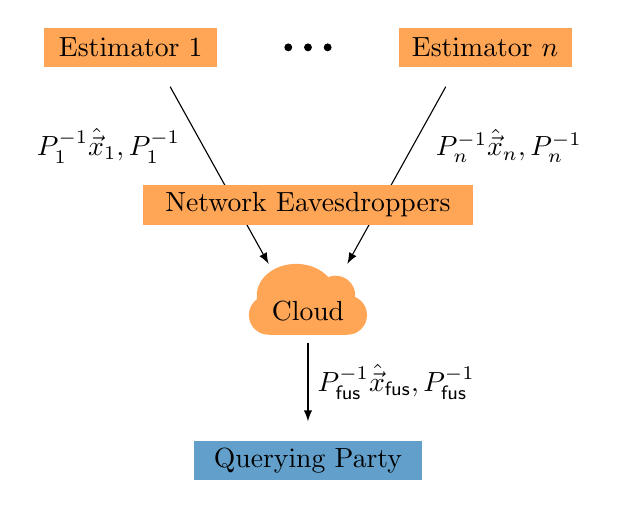
\begin{tikzpicture}
        % Estimators
        \fill [pyplotorange!70] (1.4,5.75) rectangle (3.6,5.25);
        \fill [pyplotorange!70] (5.9,5.75) rectangle (8.1,5.25);
        \node at (2.5,5.5) {Estimator $1$};
        \node at (7,5.5) {Estimator $n$};
        % Dots
        \fill [black] (5,5.5) circle (0.05);
        \fill [black] (4.5,5.5) circle (0.05);
        \fill [black] (4.75,5.5) circle (0.05);
        % Estimates
        \node [left] at (3.25,4.25) {$\mat{P}_1^{-1}\hat{\vec{x}}_1,\mat{P}_1^{-1}$};
        \node [right] at (6.25,4.25) {$\mat{P}_n^{-1}\hat{\vec{x}}_n,\mat{P}_n^{-1}$};
        % Estimator arrows
        \draw [-latex]  plot coordinates {(3,5)  (4.25,2.75)};
        \draw [-latex]  plot coordinates {(6.5,5)  (5.25,2.75)};
        % Network
        \fill [pyplotorange!70] (2.65,3.75) rectangle (6.85,3.25);
        \node at (4.75,3.5) {Network Eavesdroppers};
        % Cloud
        \fill [pyplotorange!70] (4.6,2.35) ellipse (0.5 and 0.4);
        \fill [pyplotorange!70] (5.25,2.1) ellipse (0.25 and 0.25);
        \fill [pyplotorange!70] (4.25,2.1) ellipse (0.25 and 0.25);
        \fill [pyplotorange!70] (5.1,2.35) ellipse (0.25 and 0.25);
        \fill [pyplotorange!70] (4.25,1.85) rectangle (5.25,2.1);
        \node at (4.75,2.15) {Cloud};
         % Fusion
        \node [right] at (4.75,1.25) {$\mat{P}_{\mathsf{fus}}^{-1}\hat{\vec{x}}_{\mathsf{fus}},\mat{P}_{\mathsf{fus}}^{-1}$};
        % Querying party
        \fill [pyplotblue!70] (3.3,0.5) rectangle (6.2,0);
        \node at (4.75,0.25) {Querying Party};
        % Querying party arrows
        \draw [-latex]  plot coordinates {(4.75,1.75)  (4.75,0.75)};
    \end{tikzpicture}
    \caption{Trusted (blue) and untrusted (orange) participants, and the communications between them in the cloud fusion problem.}
    \label{fig:cloud_fusion:problem_layout}
\end{figure}

% 
% 8888888888 888     888  .d8888b. 8888888 .d88888b.  888b    888      888      
% 888        888     888 d88P  Y88b  888  d88P" "Y88b 8888b   888      888      
% 888        888     888 Y88b.       888  888     888 88888b  888      888      
% 8888888    888     888  "Y888b.    888  888     888 888Y88b 888      888      
% 888        888     888     "Y88b.  888  888     888 888 Y88b888      888      
% 888        888     888       "888  888  888     888 888  Y88888      888      
% 888        Y88b. .d88P Y88b  d88P  888  Y88b. .d88P 888   Y8888      888      
% 888         "Y88888P"   "Y8888P" 8888888 "Y88888P"  888    Y888      88888888 
%                                                                               
%                                                                               
%                                                                               
% 

\section{Confidential Cloud Fusion Leaking Fusion Weights}\label{sec:cloud_fusion:secfci}
In this section, we present a method for computing the fusion result \eqref{eq:cloud_fusion:fus_info_vec_and_mat} at the fusion cloud by leaking the FCI fusion weights \eqref{eq:prelims:fci_solution} to malicious adversaries. As stated in the problem formulation, solving the fusion problem, in general, is difficult, and we make some relaxations to the cryptographic aims for this solution.
\begin{description}
    \item[Trusted sensors] In this method, we assume that sensors are trusted. That is, only the fusion cloud and eavesdroppers are considered honest-but-curious adversaries, and no sensor estimate information should be made available to them.
    \item[Leakage of fusion weights] While all estimate information available to colluding malicious parties should be encrypted with a scheme meeting the IND-CPA notion, we make an exception for the FCI fusion weights \eqref{eq:prelims:fci_solution}, which may be leaked to both the fusion cloud and eavesdroppers.
\end{description}
Here, we also note that the weakening of cryptographic guarantees caused by the leakage of fusion weights also has an upside that benefits fusion performance. The leakage of weights allows the cloud to prioritise some sensor data over others. For example, in bandwidth-limited networks, communication with sensors of lower weight, and therefore high uncertainty, may be dropped in favour of those that lead to better fusion results.

Lastly, we assume that the trusted sensors are computationally capable of locally running both the Paillier and Lewi encryption schemes, introduced in sections \ref{subsec:prelims:paillier} and \ref{subsec:prelims:lewi_ore}, and require a one-time network key distribution step before fusion of sensor data can take place at the cloud. This key distribution step consists of a trusted party generating a Paillier scheme public key pair $\mathsf{pk}$ and $\mathsf{sk}$ and a shared Lewi scheme symmetric key $\mathsf{sk}_{\mathsf{o}}$. The public key $\mathsf{pk}$ is made available to the cloud and sensors, the secret key $\mathsf{sk}$ to the querying party and the shared ORE key $\mathsf{sk}_{\mathsf{o}}$ to the sensors. The sharing of these keys can be performed by any public-key encryption scheme such as RSA [rivestMethodObtainingDigital1978].

% 
%  #######           ######  ######## ##    ## 
% ##     ##         ##    ## ##       ###   ## 
%        ##         ##       ##       ####  ## 
%  #######  #######  ######  ######   ## ## ## 
% ##                      ## ##       ##  #### 
% ##                ##    ## ##       ##   ### 
% #########          ######  ######## ##    ## 
% 

\subsection{Two-sensor Case}\label{subsec:cloud_fusion:secfci_2sen}
The confidential fusion algorithm will first be introduced in the special case of two sensors, before an extension to the $n$-sensor case. Recalling FCI fusion \eqref{eq:prelims:ci_info_vec}, \eqref{eq:prelims:ci_info_mat} and \eqref{eq:prelims:ci_weight_sum}, we can write the fusion of two information vectors and matrices as
\begin{equation}
    \mat{P}_{\mathsf{fus}}^{-1}\hat{\vec{x}}_{\mathsf{fus}} = \omega_1\mat{P}_1^{-1}\hat{\vec{x}}_1 + (1 - \omega_1)\mat{P}_2^{-1}\hat{\vec{x}}_2
\end{equation}
and
\begin{equation}
    \mat{P}_{\mathsf{fus}}^{-1} = \omega_1\mat{P}_1^{-1} + (1 - \omega_1)\mat{P}_2^{-1}\,,
\end{equation}
with $0\leq \omega_1\leq 1$, and note the suitability of addition and scalar multiplication to the Paillier scheme when the weight $\omega_1$ is known. To compute the fused information vector $\mat{P}_{\mathsf{fus}}^{-1}\hat{\vec{x}}_{\mathsf{fus}}$ and information matrix $\mat{P}_{\mathsf{fus}}^{-1}$ homomorphically, local estimate information must first be encoded as integers before encryption at the sensors. Using the Q number format in section \ref{subsec:prelims:encoding}, we let $M=N$, where $N$ is the Paillier modulus, choose an appropriate precision $\phi$ and denote encoding with $\delta$ previous multiplications as $\mathsf{E}_{\delta}(\cdot)$. Encoding, encryption and fusion with Paillier homomorphic properties \eqref{eq:prelims:paillier_hom_add} and \eqref{eq:prelims:paillier_hom_mult} is then given by
\begin{equation}\label{eq:cloud_fusion:secfci_2sen_paillier_fuse_ests}
    \mathcal{E}_{\mathsf{pk}}\left(\mathsf{E}_1\left(\mat{P}_{\mathsf{fus}}^{-1}\hat{\vec{x}}_{\mathsf{fus}}\right)\right) \approx \left(\mathsf{E}_0(\omega_1)\otimes\mathcal{E}_{\mathsf{pk}}\left(\mathsf{E}_0\left(\mat{P}^{-1}_1\hat{\vec{x}}_1\right)\right)\right)\oplus\left(\mathsf{E}_0(1 - \omega_1)\otimes\mathcal{E}_{\mathsf{pk}}\left(\mathsf{E}_0\left(\mat{P}^{-1}_2\hat{\vec{x}}_2\right)\right)\right)
\end{equation}
and
\begin{equation}\label{eq:cloud_fusion:secfci_2sen_paillier_fuse_covs}
    \mathcal{E}_{\mathsf{pk}}\left(\mathsf{E}_1\left(\mat{P}_{\mathsf{fus}}^{-1}\right)\right) \approx \left(\mathsf{E}_0(\omega_1)\otimes\mathcal{E}_{\mathsf{pk}}\left(\mathsf{E}_0\left(\mat{P}^{-1}_1\right)\right)\right)\oplus\left(\mathsf{E}_0(1 -\omega_1)\otimes\mathcal{E}_{\mathsf{pk}}\left(\mathsf{E}_0\left(\mat{P}^{-1}_2\right)\right)\right)\,,
\end{equation}
with encoding approximation errors dependent on precision parameter $\phi$. The trusted querying party can now request encryptions \eqref{eq:cloud_fusion:secfci_2sen_paillier_fuse_ests} and \eqref{eq:cloud_fusion:secfci_2sen_paillier_fuse_covs} from the cloud and decrypt them with secret key $\mathsf{sk}$.

All that remains for computing \eqref{eq:cloud_fusion:secfci_2sen_paillier_fuse_ests} and \eqref{eq:cloud_fusion:secfci_2sen_paillier_fuse_covs} in the two-sensor case is obtaining the parameter $\omega_1$ at the cloud. Since $\omega_1$ depends on the estimate errors of both sensors it cannot be computed locally and requires appropriate leakage to the cloud. This is achieved by using the Lewi ORE scheme and encrypting discretised sequences whose intersection can be used to compute the two-sensor FCI fusion weight constraint \eqref{eq:prelims:fci_added_constraints}, namely
\begin{equation}\label{eq:cloud_fusion:secfci_2sen_intersect_cond}
    \omega_1\tr(\mat{P}_1) = (1-\omega_1)\tr(\mat{P}_2)\,.
\end{equation}
To evaluate \eqref{eq:cloud_fusion:secfci_2sen_intersect_cond} with comparisons at the cloud, a public stepsize $g\leq 1$ is chosen, such that $1/g \in \mathbb{N}$, and both sensors discretise the weight $0\leq\omega_1\leq 1$ and compute resulting sequences of either side of the equality in \eqref{eq:cloud_fusion:secfci_2sen_intersect_cond}. This results in the sequence
\begin{equation}\label{eq:cloud_fusion_secfci_2sen_seq_1}
    \left\langle0, g\tr(\mat{P}_1), 2g\tr(\mat{P}_1),\dots,\tr(\mat{P}_1)\right\rangle
\end{equation}
at sensor $1$ and
\begin{equation}\label{eq:cloud_fusion_secfci_2sen_seq_2}
    \left\langle\tr(\mat{P}_2), (1-g)\tr(\mat{P}_2), (1-2g)\tr(\mat{P}_2),\dots,0\right\rangle
\end{equation}
at sensor $2$. Comparison of same-index values in the sequences \eqref{eq:cloud_fusion_secfci_2sen_seq_1} and \eqref{eq:cloud_fusion_secfci_2sen_seq_2} leads to the bounds $\iota g<\omega_1<(\iota+1)g$, for some index $\iota$, that can be used to approximate the true solution as $\hat{\omega}_1 = \iota g+g/2 \approx \omega_1$, or in the case of an equality, $\hat{\omega}_1 = \iota g = \omega_1$. To obtain this approximation without additional leakage, elements in \eqref{eq:cloud_fusion_secfci_2sen_seq_1} and \eqref{eq:cloud_fusion_secfci_2sen_seq_2} are encrypted with the ORE key $\mathsf{sk}_{\mathsf{o}}$. As no homomorphic operations are performed with the scheme an arbitrary precision integer encoding can be used and is neglected from the notation below. The sequence produced by sensor $1$ is therefore given by
\begin{equation}\label{eq:cloud_fusion:secfci_2sen_enc_seq_1}
    \left\langle\mathcal{E}^{\mathsf{L}}_{\mathsf{sk}_{\mathsf{o}}}(0), \mathcal{E}^{\mathsf{L}}_{\mathsf{sk}_{\mathsf{o}}}(g\tr(\mat{P}_1)), \mathcal{E}^{\mathsf{L}}_{\mathsf{sk}_{\mathsf{o}}}(2g\tr(\mat{P}_1)),\dots,\mathcal{E}^{\mathsf{L}}_{\mathsf{sk}_{\mathsf{o}}}(\tr(\mat{P}_1))\right\rangle
\end{equation}
and that by sensor $2$ by
\begin{equation}\label{eq:cloud_fusion:secfci_2sen_enc_seq_2}
    \left\langle\mathcal{E}^{\mathsf{R}}_{\mathsf{sk}_{\mathsf{o}}}(\tr(\mat{P}_2)), \mathcal{E}^{\mathsf{R}}_{\mathsf{sk}_{\mathsf{o}}}((1-g)\tr(\mat{P}_2)), \mathcal{E}^{\mathsf{R}}_{\mathsf{sk}_{\mathsf{o}}}((1-2g)\tr(\mat{P}_2)),\dots,\mathcal{E}^{\mathsf{R}}_{\mathsf{sk}_{\mathsf{o}}}(0)\right\rangle\,,
\end{equation}
where we note the difference between \textit{left} and \textit{right} encryptions for each sensor, allowing comparisons between sequences. Efficiently findable using a binary search, the approximate solution when comparing elements of the two sequences can be seen graphically in figure \ref{fig:cloud_fusion:secfci_2sen_intersect}, where the approximation is taken as halfway between consecutive comparisons that change sign.
\begin{figure}[htbp]
    \begin{center}
       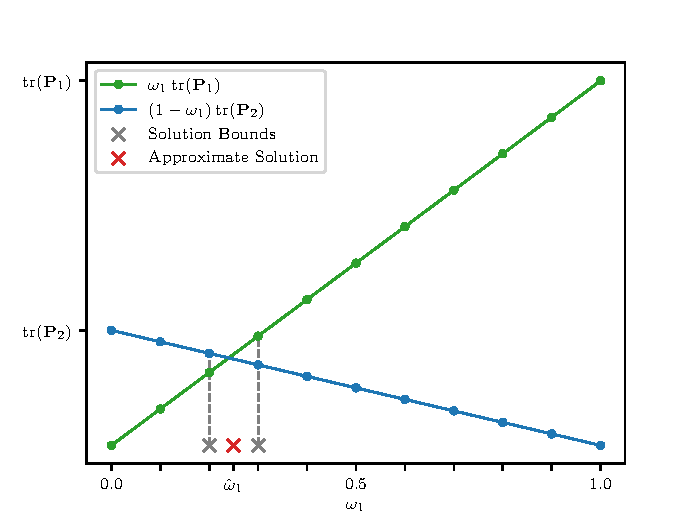
\includegraphics{figures/cloud_fusion_secfci_2sen_intersect.pdf}
    \end{center}
    \caption{Approximation of $\omega_1$ with stepsize $g=0.1$. Comparisons are only possible when $\omega_1$ is a multiple of $g$ (points on the graphs).}
    \label{fig:cloud_fusion:secfci_2sen_intersect}
    % TODO to figure. Y-axis should have 2 points, for trP1 and trP2. Omega^x should be omega_1. Make larger. Add a hat to the approximation of omega
 \end{figure}

In this way, computing fusion on the cloud homomorphically can be performed when having access to only local encryptions of information vectors and matrices, \eqref{eq:cloud_fusion:secfci_2sen_paillier_fuse_covs} and \eqref{eq:cloud_fusion:secfci_2sen_paillier_fuse_ests}, in addition to the sequences of order-revealing encryptions \eqref{eq:cloud_fusion:secfci_2sen_enc_seq_1} and \eqref{eq:cloud_fusion:secfci_2sen_enc_seq_2} that leak an approximation $\hat{\omega}_1 \approx \omega_1$.

% 
% ##    ##          ######  ######## ##    ## 
% ###   ##         ##    ## ##       ###   ## 
% ####  ##         ##       ##       ####  ## 
% ## ## ## #######  ######  ######   ## ## ## 
% ##  ####               ## ##       ##  #### 
% ##   ###         ##    ## ##       ##   ### 
% ##    ##          ######  ######## ##    ## 
% 

\subsection{Multi-sensor Case}\label{subsec:cloud_fusion:secfci_nsen}
To compute the fusion of $n$ sensor estimates in the information form we want the solutions to
\begin{equation}
    \mat{P}_{\mathsf{fus}}^{-1}\hat{\vec{x}}_{\mathsf{fus}} = \sum_{i=1}^n\omega_i\mat{P}_i^{-1}\hat{\vec{x}}_i
\end{equation}
and
\begin{equation}
    \mat{P}_{\mathsf{fus}}^{-1} = \sum_{i=1}^n\omega_i\mat{P}_i^{-1}\,.
\end{equation}
When the fusion weights $\omega_i$, $1\leq i\leq n$, $\sum_{i=1}^n\omega_i=1$, are known, we can again use the appropriate integer encoding and Paillier homomorphic properties to compute the fusion homomorphically as
\begin{equation}\label{eq:cloud_fusion:secfci_nsen_paillier_fuse_ests}
    \mathcal{E}_{\mathsf{pk}}\left(\mathsf{E}_1\left(\mat{P}_{\mathsf{fus}}^{-1}\hat{\vec{x}}_{\mathsf{fus}}\right)\right) \approx \oplus_{i=1}^n\left(\mathsf{E}_0(\omega_i)\otimes\mathcal{E}_{\mathsf{pk}}\left(\mathsf{E}_0\left(\mat{P}^{-1}_i\hat{\vec{x}}_i\right)\right)\right)
\end{equation}
and
\begin{equation}\label{eq:cloud_fusion:secfci_nsen_paillier_fuse_covs}
    \mathcal{E}_{\mathsf{pk}}\left(\mathsf{E}_1\left(\mat{P}_{\mathsf{fus}}^{-1}\right)\right) \approx \oplus_{i=1}^n\left(\mathsf{E}_0(\omega_i)\otimes\mathcal{E}_{\mathsf{pk}}\left(\mathsf{E}_0\left(\mat{P}^{-1}_i\right)\right)\right)\,.
\end{equation}
What remains is to compute the weights $\omega_i$ at the cloud such that the $n$-sensor FCI conditions \eqref{eq:prelims:fci_added_constraints} are met. Similar to the two-sensor case, we can use sequences of order-revealing encryptions to leak an approximation to this result. 

Each condition \eqref{eq:prelims:fci_added_constraints} is considered as a partial problem, that is,
\begin{equation}\label{eq:cloud_fusion:secfci_nsen_partial_sol_subspace}
    \omega_i\tr(\mat{P}_i) = \omega_{i+1}\tr(\mat{P}_{i+1})\,,
\end{equation}
with $1\leq i< n$ and $\sum_{i=1}^n\omega_i=1$, and their solution spaces, linear subspaces $\mathcal{S}_i$ over possible values of $\vec{\omega}=\begin{bsmallmatrix}\omega_1 & \cdots & \omega_n\end{bsmallmatrix}^\top$, desired. The intersection of these subspaces naturally results in the final solution to $\vec{\omega}$ in \eqref{eq:prelims:fci_matrix_equation}. Each solution space $\mathcal{S}_i$ can be defined by $n-1$ linearly independent solution points $\vec{\omega}_i^{(\zeta)}$, $1\leq \zeta\leq n-1$. $n-2$ of these solutions can be trivially obtained as the points where a single $\omega_j=1$, $j\neq i\neq i+1$ while the final point, $\vec{\omega}_i^{(n-1)}$, can be obtained as the solution to
\begin{equation}\label{eq:cloud_fusion:secfci_nsen_partial_sol_point}
    \omega_i\tr(\mat{P}_i) = (1-\omega_i)\tr(\mat{P}_{i+1})\,,
\end{equation}
$\omega_j=0$, $j\neq i\neq i+1$, noting equivalence to \eqref{eq:cloud_fusion:secfci_nsen_partial_sol_subspace} and $\omega_{i+1}=1-\omega_i$. The solutions $\vec{\omega}_i^{(\zeta)}$ and the $n-2$ dimensional subspace they define can be rewritten in parametric form as
\begin{equation}\label{eq:cloud_fusion:secfci_nsen_partial_subspace}
    \mathcal{S}_i(\vec{\gamma}_i)=\vec{\omega}_i^{(1)} + 
    \begin{bmatrix}
        \bar{\vec{\omega}}_i^{(2)} & \cdots & \bar{\vec{\omega}}_i^{(n-1)}
    \end{bmatrix}
    \vec{\gamma}_i\,,
\end{equation}
where $\bar{\vec{\omega}}_i^{(\zeta)}=\vec{\omega}_i^{(\zeta)}-\vec{\omega}_i^{(1)}$ denotes direction vectors. The intersection of these $n-1$ subspaces gives the solution to $\vec{\omega}$ in \eqref{eq:prelims:fci_matrix_equation}. This solution, as well as the parameters $\vec{\gamma}_i$, can be obtained as a solution to the linear system
\begin{equation}\label{eq:cloud_fusion:secfci_nsen_omega_solution}
    \begin{bmatrix}
        -\mat{I} & \bar{\vec{\omega}}_1^{(2)} & \cdots & \bar{\vec{\omega}}_1^{(n-1)} & 0 & \cdots & 0\\
        \vdots & 0 &  & \ddots &  & \ddots & \vdots\\
        \vdots & \vdots & \ddots &  & \ddots &  & 0\\
        -\mat{I} & 0 & \cdots & 0 & \bar{\vec{\omega}}_{n-1}^{(2)} & \cdots & \bar{\vec{\omega}}_{n-1}^{(n-1)}
    \end{bmatrix}
    \begin{bmatrix}
        \vec{\omega}\\
        \vec{\gamma}_1\\
        \vdots\\
        \vec{\gamma}_{n-1}\\
    \end{bmatrix}=
    \begin{bmatrix}
        -\vec{\omega}_1^{(1)}\\
        \vdots\\
        -\vec{\omega}_{n-1}^{(1)}\\
    \end{bmatrix}\,.
\end{equation}

Therefore, to compute \eqref{eq:cloud_fusion:secfci_nsen_omega_solution} at the cloud leaking only comparisons required to compute the fusion weights, we approximate the solutions to \eqref{eq:cloud_fusion:secfci_nsen_partial_sol_point} with ORE sequences similar to the two-sensor case. Each sensor $i$ uses $\mathsf{sk}_{\mathsf{o}}$ to encrypt the discretisation 
\begin{equation}\label{eq:cloud_fusion:secfci_nsen_enc_seqs}
    \begin{split}
        \left\langle\mathcal{E}^{\mathsf{L}}_{\mathsf{sk}_{\mathsf{o}}}(0), \mathcal{E}^{\mathsf{L}}_{\mathsf{sk}_{\mathsf{o}}}(g\tr(\mat{P}_i)), \mathcal{E}^{\mathsf{L}}_{\mathsf{sk}_{\mathsf{o}}}(2g\tr(\mat{P}_i)),\dots,\mathcal{E}^{\mathsf{L}}_{\mathsf{sk}_{\mathsf{o}}}(\tr(\mat{P}_i))\right\rangle\,,\ & \text{if } i \text{ is odd, or}\\
        \left\langle\mathcal{E}^{\mathsf{R}}_{\mathsf{sk}_{\mathsf{o}}}(0), \mathcal{E}^{\mathsf{R}}_{\mathsf{sk}_{\mathsf{o}}}(g\tr(\mat{P}_i)), \mathcal{E}^{\mathsf{R}}_{\mathsf{sk}_{\mathsf{o}}}(2g\tr(\mat{P}_i)),\dots,\mathcal{E}^{\mathsf{R}}_{\mathsf{sk}_{\mathsf{o}}}(\tr(\mat{P}_i))\right\rangle\,,\ & \text{if } i \text{ is even,}
    \end{split}
\end{equation}
allowing for comparison between sequences from consecutive sensors $i$ and $i+1$. To approximate the solution to each \eqref{eq:cloud_fusion:secfci_nsen_partial_sol_point}, the sequence from sensor $i+1$ is reversed,
\begin{equation}\label{eq:cloud_fusion:secfci_nsen_enc_seqs_reversed}
    \begin{split}
        \left\langle\mathcal{E}^{\mathsf{L}}_{\mathsf{sk}_{\mathsf{o}}}(\tr(\mat{P}_i)),\mathcal{E}^{\mathsf{L}}_{\mathsf{sk}_{\mathsf{o}}}((1-g)\tr(\mat{P}_i)), \mathcal{E}^{\mathsf{L}}_{\mathsf{sk}_{\mathsf{o}}}((1-2g)\tr(\mat{P}_i)),\dots,\mathcal{E}^{\mathsf{L}}_{\mathsf{sk}_{\mathsf{o}}}(0)\right\rangle\,,\ & \text{if } i \text{ is odd, or}\\
        \left\langle\mathcal{E}^{\mathsf{R}}_{\mathsf{sk}_{\mathsf{o}}}(\tr(\mat{P}_i)), \mathcal{E}^{\mathsf{R}}_{\mathsf{sk}_{\mathsf{o}}}((1-g)\tr(\mat{P}_i)), \mathcal{E}^{\mathsf{R}}_{\mathsf{sk}_{\mathsf{o}}}((1-2g)\tr(\mat{P}_i)),\dots,\mathcal{E}^{\mathsf{R}}_{\mathsf{sk}_{\mathsf{o}}}(0)\right\rangle\,,\ & \text{if } i \text{ is even,}
    \end{split}
\end{equation}
resulting in sequences of the same form as \eqref{eq:cloud_fusion:secfci_2sen_enc_seq_1} and \eqref{eq:cloud_fusion:secfci_2sen_enc_seq_2}. The value $\hat{\omega}_i = \iota g + g/2 \approx \omega_i$, or in the case of an equality $\hat{\omega}_i = \iota g = \omega_i$, for some index $\iota$, is used to approximate the solution $\hat{\vec{\omega}}_i^{(n-1)} \approx \vec{\omega}_i^{(n-1)}$. A visualisation of solving \eqref{eq:cloud_fusion:secfci_nsen_omega_solution} with approximations to \eqref{eq:cloud_fusion:secfci_nsen_partial_sol_point} in the three-sensor case is graphically shown in figure \ref{fig:cloud_fusion:secfci_nsen_partial_sols_and_intersect}.
\begin{figure}[htbp]
    \begin{subfigure}[htbp]{\textwidth}
        \begin{center}
            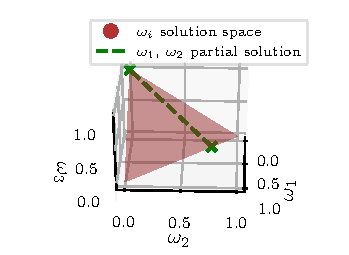
\includegraphics{figures/partial_sol1.pdf}
        \end{center}
        \caption{Approximated solution space \eqref{eq:cloud_fusion:secfci_nsen_partial_subspace} when $i=1$.}
        \label{fig:3_sensor_partial_sol}
    \end{subfigure}
    \hfill
    \begin{subfigure}[htbp]{\textwidth}
        \begin{center}
            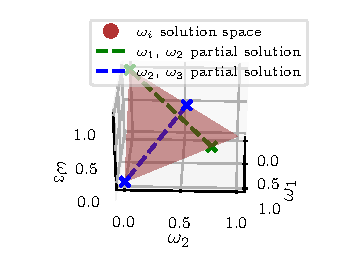
\includegraphics{figures/partial_sols.pdf}
        \end{center}
        \caption{Approximated solution space \eqref{eq:cloud_fusion:secfci_nsen_partial_subspace} when $i=2$.}
        \label{fig:3_sensor_partial_sols}
    \end{subfigure}
    \hfill
    \begin{subfigure}[htbp]{\textwidth}
        \begin{center}
            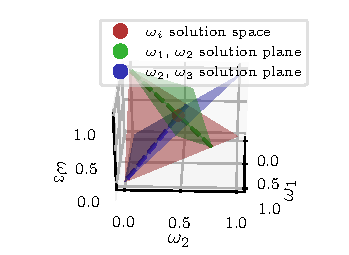
\includegraphics{figures/partial_sol_planes.pdf}
        \end{center}
        \caption{Intersection of partial solutions spaces gives fusion weights $\vec{\omega}$ in \eqref{eq:prelims:fci_matrix_equation}.}
        \label{fig:3sen_planes}
    \end{subfigure}
    \caption{Solving fusion weights $\vec{\omega}$ with approximations to \eqref{eq:cloud_fusion:secfci_nsen_partial_sol_point}.}
    \label{fig:cloud_fusion:secfci_nsen_partial_sols_and_intersect}
    % TODO Label which points are approximated. Turn axis labels the right way around. Label solution space correctly; it is the plane of the sum equalling one.
\end{figure}

The resulting estimate $\hat{\vec{\omega}} \approx \vec{\omega}$ can then be used with \eqref{eq:cloud_fusion:secfci_nsen_paillier_fuse_ests} and \eqref{eq:cloud_fusion:secfci_nsen_paillier_fuse_covs} to compute the fusion of $n$ information vectors and matrices at the cloud.

% 
%  ######   #######  ##     ## ########  
% ##    ## ##     ## ###   ### ##     ## 
% ##       ##     ## #### #### ##     ## 
% ##       ##     ## ## ### ## ########  
% ##       ##     ## ##     ## ##        
% ##    ## ##     ## ##     ## ##        
%  ######   #######  ##     ## ##        
% 

\subsection{Computational Complexity}\label{subsec:cloud_fusion:secfci_comp_complexity}
The method introduced allows the computation of FCI by using the Paillier and Lewi encryption schemes. Naturally, relying on encryption and homomorphic operations increases the complexity of computing this fusion at the sensor, cloud and querying party. Here, we look at the computational complexity of the method in terms of the required operations at each party. We assume that both the Lewi and Paillier schemes use the same key size, typically measured in bits, $\log{N}$, where $N$ is the Paillier modulus defined in section \ref{subsec:prelims:paillier}. In addition, we note the distinction between floating-point or small integer operations, treated as having runtime $O(1)$, and large integer operations with runtime dependent on bit length. While hardware architecture exists for faster encryption operations [gueronIntelAdvancedEncryption2010], we consider software implementations and treat large integer operations in terms of bit operations explicitly.

Individual encryption operation complexities with the assumptions made above have been summarised in table \ref{tab:cloud_fusion:secfci_op_complexity}. 
\begin{table}[htbp]
    \centering
    \caption{Computation complexity of involved encryption operations.}
    \label{tab:cloud_fusion:secfci_op_complexity}
    \begin{tabular}{|c|c|}
        \hline
        \textbf{Operation} & \textbf{Complexity} \\ 
        \hline
        Paillier Encryption & $O(\log^3{N})$ \\ 
        Paillier Decryption & $O(\log^3{N})$ \\ 
        Paillier Addition & $O(\log^2{N})$ \\ 
        Paillier Scalar Multiplication & $O(\log^3{N})$ \\ 
        Lewi \textit{Left} Encryption & $O(\log^2{N})$ \\ 
        Lewi \textit{Right} Encryption & $O(\log^2{N})$ \\ 
        Lewi Comparison & $O(\log^2{N})$ \\ 
        \hline
    \end{tabular}
\end{table}
Applying operation complexities to the fusion algorithm we get the computational complexity for the sensors, cloud and querying party. These can be seen in table \ref{tab:cloud_fusion:secfci_complexity}, where unencrypted FCI algorithm complexities are also shown for reference. 
\begin{table}[htbp]
   \centering
   \caption{Computation complexity for each party.}
   \label{tab:cloud_fusion:secfci_complexity}
   \begin{tabular}{|c|c|c|}
      \hline
       & \textbf{FCI} & \textbf{Confidential Fusion Leaking Weights} \\ 
      \hline
      Sensor & $O(1)$ & $O\left(d^2\log^3{N} + \frac{1}{g}\log^2{N}\right)$ \\ 
      Cloud & $O\left(nd^2+n^3\right)$ & $O\left(nd^2\log^3{N} + n\log{\frac{1}{g}} + n^3\right)$ \\ 
      Querying Party & $O(1)$ & $O\left(d^2\log^3{N}\right)$ \\ 
      \hline
   \end{tabular}
\end{table}
These complexities show the additional computational cost required for providing the security benefits of the presented scheme and must naturally be reflected in chosen hardware when developing a system where the benefits are desired.

% 
%  ######  ########  ######  
% ##    ## ##       ##    ## 
% ##       ##       ##       
%  ######  ######   ##       
%       ## ##       ##       
% ##    ## ##       ##    ## 
%  ######  ########  ######  
% 

\subsection{Security Analysis}\label{subsec:cloud_fusion:secfci_security}
Recalling the cryptographic aims of the estimate fusion problem introduced in the problem formulation and weakened for the presented method, we desire estimate information to be encrypted with a notion meeting IND-CPA at the fusion cloud and eavesdroppers while allowing the leakage of fusion weights, and naturally any functions derivable only from this information.

Since Paillier encryptions \eqref{eq:cloud_fusion:secfci_nsen_paillier_fuse_ests} and \eqref{eq:cloud_fusion:secfci_nsen_paillier_fuse_covs} meet the IND-CPA notion, this information meets the desired aims. The remaining available information to the cloud and eavesdroppers are the sequences encrypted by the Lewi ORE scheme. This scheme meets the simulation-based security discussed in section \ref{subsec:prelims:lewi_ore} and is shown in section \ref{subsec:cloud_fusion:secfci_nsen} to correspond to the leakage of approximations to the weights $\omega_i$, in addition to some leakage beyond the used ciphertext order comparisons due to the relaxation of the IND-OCPA notation (which can be difficult to quantify in context). Lastly, we also acknowledge an implicit leakage of estimate dimension $d$ associated with the use of elementwise encryption. Although methods for homomorphic encryption of vectors exist [alexandruPrivateWeightedSum2020], we leave this as future work on this topic and note that the dimension $d$ may leak information about the data fusion use case but that estimates themselves remain encrypted.

The leakages present in the introduced method, namely the leakage of fusion weights and estimate dimensions, may lead to inferences about sensor hardware and must naturally be considered when planning the implementation of this method in a real-world system.

% 
%  ######  #### ##     ## 
% ##    ##  ##  ###   ### 
% ##        ##  #### #### 
%  ######   ##  ## ### ## 
%       ##  ##  ##     ## 
% ##    ##  ##  ##     ## 
%  ######  #### ##     ## 
% 

\subsection{Simulation}\label{subsec:cloud_fusion:secfci_simulation}
Along with the discussions above, we have implemented a simulation of the method to demonstrate its fusion accuracy when compared to the FCI algorithm on a trusted cloud. A constant-speed linear system, 
\begin{equation}\label{eq:cloud_fusion:secfci_system_model}
    \vec{x}_{k+1} = 
    \begin{bmatrix}
        1 & 0.5 & 0 & 0\\
        0 & 1 & 0 & 0\\
        0 & 0 & 1 & 0.5\\
        0 & 0 & 0 & 1
    \end{bmatrix}\vec{x}_k + \vec{w}_k\,,\qquad \vec{w}_k\sim\mathcal{N}\left(\vec{0},
    \begin{bmatrix}
        0.4 & 1.3 & 0 & 0\\
        1.3 & 5.0 & 0 & 0\\
        0 & 0 & 0.4 & 1.3\\
        0 & 0 & 1.3 & 5.0
    \end{bmatrix}
    \right)\,,
\end{equation}
was simulated and measured by four independent position sensors $1\leq i\leq 4$, that produced measurements 
\begin{equation}\label{eq:cloud_fusion:secfci_measurement_model}
    \vec{z}_{k,i} = 
    \begin{bmatrix}
        1 & 0 & 0 & 0\\
        0 & 0 & 1 & 0
     \end{bmatrix}\vec{x}_k + \vec{v}_{k,i}\,,\qquad \vec{v}_{k,i}\sim\mathcal{N}\left(\vec{0},\mat{R}_i\right)\,,
\end{equation}
with covariances sampled independently, resulting in
\begin{equation}\label{eq:cloud_fusion:secfci_measurement_model_covariances}
    \begin{split}
        &\mat{R}_1 = 
        \begin{bmatrix}
            4.77 & -0.15\\
            -0.15 & 4.94
        \end{bmatrix}\,,\\
        &\mat{R}_2 = 
        \begin{bmatrix}
            2.99 & -0.55\\
            -0.55 & 4.44
        \end{bmatrix}\,,\\
        &\mat{R}_3 = 
        \begin{bmatrix}
            2.06 & 0.68\\
            0.68 & 1.96
        \end{bmatrix}\text{ and }\\
        &\mat{R}_4 = 
        \begin{bmatrix}
            1.17 & 0.80\\
            0.80 & 0.64
        \end{bmatrix}\,.
    \end{split}
\end{equation}
Each sensor ran a local linear Information Filter (IF) from section \ref{subsec:prelims:if} before processing and sending its estimate information, $\mat{P}_{k, i}^{-1}\hat{\vec{x}}_{k, i}$ and $\mat{P}_{k, i}^{-1}$, to the cloud for fusion. At each timestep, time-independent fusion of information vectors and matrices was computed homomorphically at the cloud and decrypted by the querying party. The simulation was written in the Python and C programming languages, using the $\mathsf{phe}$ Paillier encryption scheme library [PythonPaillier2013], and using a key size of $512$ bits for encryption schemes. Figure \ref{fig:cloud_fusion:secfci_sim_error} shows the average estimation error of $1000$ simulations when using our algorithm with varying stepsizes $g$ alongside the standard FCI algorithm. 
\begin{figure}[htbp]
    \centering
    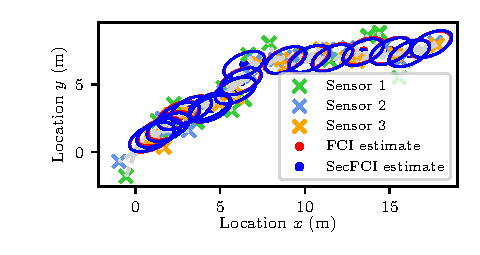
\includegraphics{figures/fci_secfci_cmp.pdf}
    \caption{Average MSE with varying stepsize $g$ over $1000$ simulation runs.}
    \label{fig:cloud_fusion:secfci_sim_error}
    % TODO figure to display MSE of 1000 simulations for FCI and our method with g=0.1, 0.2, 0.33, 0.5
    % latex y-axis label for MSE
 \end{figure}
 In all cases, resulting plaintext information vectors and matrices were converted to estimates and estimate error covariances before comparison with the true simulated state. From the figure, it can be seen that the estimation error of our method is similar to the normal FCI method when stepsize $g$ is small, $g\leq 2$, but grows as expected when $g$, and thus the possible error in weights $\omega_i$, is increased.

Since the system described by \eqref{eq:cloud_fusion:secfci_system_model}, \eqref{eq:cloud_fusion:secfci_measurement_model} and estimated by the KF reaches an estimation steady-state, fusion weights $\omega_i$ do as well. Figure \ref{fig:cloud_fusion:secfci_omega_error} shows the steady state error of estimated weights when compared to the true FCI weights. 
\begin{figure}[htbp]
    \centering
    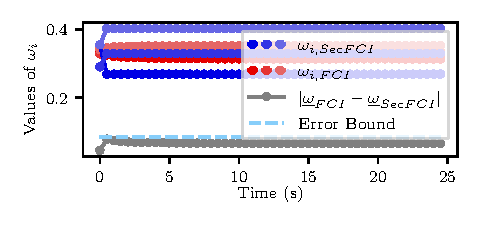
\includegraphics{figures/omegas_cmp.pdf}
    \caption{Steady-state MSE of estimated weights $\hat{\vec{\omega}}$ with varying stepsize $g$.}
    \label{fig:cloud_fusion:secfci_omega_error}
    % TODO plot steady-state error of weights g=0.1,0,2,0.33,0.5
    % Y-axis is weight error (not simulation error) and X-axis is g
\end{figure}
Here, the maximum errors in fusion weights naturally depend on the stepsize $g$ and support the results seen in figure \ref{fig:cloud_fusion:secfci_sim_error}. Further, an upper bound on this error can be derived by considering the maximum error of each approximation \eqref{eq:cloud_fusion:secfci_nsen_partial_sol_point} and is given by
\begin{equation}
    \left|\hat{\vec{\omega}} - \vec{\omega}\right| \leq \frac{g}{2}\sqrt{n}\,.
\end{equation}

% 
% 8888888888 888     888  .d8888b. 8888888 .d88888b.  888b    888      888b    888 888      
% 888        888     888 d88P  Y88b  888  d88P" "Y88b 8888b   888      8888b   888 888      
% 888        888     888 Y88b.       888  888     888 88888b  888      88888b  888 888      
% 8888888    888     888  "Y888b.    888  888     888 888Y88b 888      888Y88b 888 888      
% 888        888     888     "Y88b.  888  888     888 888 Y88b888      888 Y88b888 888      
% 888        888     888       "888  888  888     888 888  Y88888      888  Y88888 888      
% 888        Y88b. .d88P Y88b  d88P  888  Y88b. .d88P 888   Y8888      888   Y8888 888      
% 888         "Y88888P"   "Y8888P" 8888888 "Y88888P"  888    Y888      888    Y888 88888888 
%                                                                                           
%                                                                                           
%                                                                                           
% 

\section{Confidential Cloud Fusion Without Leaking Fusion Weights}\label{sec:cloud_fusion:secfci2}
Previously, we presented a method for solving the estimate fusion problem by weakening the desired cryptographic aims in section \ref{sec:cloud_fusion:problem}. In this section, we present a method that meets these aims exactly by making a relaxation on the produced fusion output of the fusion cloud.
\begin{description}
    \item[Broader fusion output] In this method, the fusion cloud is not strictly required to produce the fused information vector $\mat{P}_{\mathsf{fus}}^{-1}\hat{\vec{x}}_{\mathsf{fus}}$ and matrix $\mat{P}_{\mathsf{fus}}^{-1}$. Instead, any statistics over data from individual sensors $i$ can be computed homomorphically at the fusion cloud and provided to the querying party. For example, the sum statistic over inverted estimate covariance traces, $\sum_{i=1}^n \tr(\mat{P}_i)^{-1}$, may be returned.
\end{description}

The idea behind the method is to postpone the evaluation of operations that cannot be performed homomorphically until partial fusion results are decrypted by the querying party. The remaining operations are then evaluated on unencrypted inputs to produce the final fusion results. First, we note that FCI fusion \eqref{eq:prelims:ci_info_vec}, \eqref{eq:prelims:ci_info_mat} and \eqref{eq:prelims:fci_solution} can be rearranged and weights substituted to obtain
\begin{equation}\label{eq:cloud_fusion:secfci2_info_vec_rearrange}
    \mat{P}_{\mathsf{fus}}^{-1}\hat{\vec{x}}_{\mathsf{fus}} = \left(\sum_{i=1}^n \frac{1}{\tr(\mat{P}_i)}\right)^{-1}\sum_{i=1}^n\frac{1}{\tr(\mat{P}_i)}\mat{P}_i^{-1}\hat{\vec{x}}_i
\end{equation}
and
\begin{equation}\label{eq:cloud_fusion:secfci2_info_mat_rearrange}
    \mat{P}_{k,\mathsf{fus}}^{-1} = \left(\sum_{i=1}^n \frac{1}{\tr(\mat{P}_i)}\right)^{-1}\sum_{i=1}^n \frac{1}{\tr(\mat{P}_i)}\mat{P}_i^{-1}\,.
\end{equation}

In this form, innermost summations  
\begin{equation}
    \sum_{i=1}^n \frac{1}{\tr(\mat{P}_i)}\,,\ \sum_{i=1}^n \frac{1}{\tr(\mat{P}_i)}\mat{P}_i^{-1}\text{ and }\sum_{i=1}^n\frac{1}{\tr(\mat{P}_i)}\mat{P}_i^{-1}\hat{\vec{x}}_i
\end{equation}
combine information from individual sensors $i$, are computable homomorphically given suitable encryption and suit the fusion relaxation defined above. Encryptions of these sums can then be decrypted by the querying party, before remaining inversions and multiplications in \eqref{eq:cloud_fusion:secfci2_info_vec_rearrange} and \eqref{eq:cloud_fusion:secfci2_info_mat_rearrange} can be computed to obtain the final results. To depict this straightforward process, pseudocode for the encryption at the sensors, fusion at the cloud and decryption at the querying party are shown in algorithms \ref{alg:cloud_fusion:secfci2_sensor_steps}, \ref{alg:cloud_fusion:secfci2_cloud_steps} and \ref{alg:cloud_fusion:secfci2_query_steps}, respectively. As in the previous section, the Paillier encryption scheme, producing keys $\mathsf{pk}$ and $\mathsf{sk}$, is used, encoding from section \ref{subsec:prelims:encoding} is used with $M=N$, where $N$ is the Paillier scheme modulus, and an appropriate precision $\phi$ is chosen.
\begin{algorithm}[htbp]
\caption{Encryption at the Sensors}\label{alg:cloud_fusion:secfci2_sensor_steps}
\begin{algorithmic}[1]
    \setstretch{1.35}
    \Procedure{Estimate}{$i$, $\mathsf{pk}$}
    \State Estimate $\mat{P}_i^{-1}\hat{\vec{x}}_i$ locally
    \State Estimate $\mat{P}_i^{-1}$ locally
    \LineComment{Encode and encrypt scaling, covariance and estimate components}
    \State $s_i \gets \mathcal{E}_{\mathsf{pk}}\left(\mathsf{E}_{0}\left(\frac{1}{\tr(\mat{P}_i)}\right)\right)$
    \State $\mat{C}_i \gets \mathcal{E}_{\mathsf{pk}}\left(\mathsf{E}_{0}\left(\frac{1}{\tr(\mat{P}_i)}\mat{P}_i^{-1}\right)\right)$
    \State $\vec{e}_i \gets \mathcal{E}_{\mathsf{pk}}\left(\mathsf{E}_{0}\left(\frac{1}{\tr(\mat{P}_i)}\mat{P}_i^{-1}\hat{\vec{x}}_i\right)\right)$
    \State Send $s_i$, $\mat{C}_i$ and $\vec{e}_i$ to fusion cloud
    \EndProcedure
\end{algorithmic}
\end{algorithm}
\begin{algorithm}[htbp]
\caption{Partial Fusion at the Cloud}\label{alg:cloud_fusion:secfci2_cloud_steps}
\begin{algorithmic}[1]
    \setstretch{1.35}
    \Procedure{PartialFuse}{$\mathsf{pk}$}
    \State Receive $s_i$, $\mat{C}_i$ and $\vec{e}_i$ for all $1\leq i \leq n$
    \LineComment{Perform homomorphic summations}
    \State $s \gets \oplus_{i=1}^{n} s_i$
    \State $\mat{C} \gets \oplus_{i=1}^{n} \mat{C}_i$
    \State $\vec{e} \gets \oplus_{i=1}^{n} \vec{e}_i$
    \State Store $s$, $\mat{C}$ and $\vec{e}$ in case of query
    \EndProcedure
\end{algorithmic}
\end{algorithm}
\begin{algorithm}[htbp]
\caption{Completing Fusion at the Querying Party}\label{alg:cloud_fusion:secfci2_query_steps}
\begin{algorithmic}[1]
    \setstretch{1.35}
    \Procedure{QueryFuse}{$\mathsf{pk}$, $\mathsf{sk}$}
    \State Query and receive $s$, $\mat{C}$ and $\vec{e}$ from fusion cloud
    \LineComment Decrypt and decode
    \State $\bar{s} \gets \mathsf{E}^{-1}_{0}\left(\mathcal{D}_{\mathsf{pk},\mathsf{sk}}\left(s\right)\right)$
    \State $\bar{\mat{C}} \gets \mathsf{E}^{-1}_{0}\left(\mathcal{D}_{\mathsf{pk},\mathsf{sk}}\left(\mat{C}\right)\right)$
    \State $\bar{\vec{e}} \gets \mathsf{E}^{-1}_{0}\left(\mathcal{D}_{\mathsf{pk},\mathsf{sk}}\left(\vec{e}\right)\right)$
    \LineComment Compute remaining fusion operations
    \State $\mat{P}_{\mathsf{fus}}^{-1}\hat{\vec{x}}_{\mathsf{fus}} \gets \bar{s}^{-1} \cdot \bar{\vec{e}}$
    \State $\mat{P}_{\mathsf{fus}}^{-1} \gets \bar{s}^{-1} \cdot \bar{\mat{C}}$
    \State \Return $\mat{P}_{\mathsf{fus}}^{-1}\hat{\vec{x}}_{\mathsf{fus}}$, $\mat{P}_{\mathsf{fus}}^{-1}$
    \EndProcedure
\end{algorithmic}
\end{algorithm}

Along with allowing the summations to be performed homomorphically on the cloud, we note that this form of the FCI also allows the cloud's partial fusion operations to be evaluated sequentially. This can be seen in algorithm \ref{alg:cloud_fusion:secfci2_cloud_steps}, where individual components $s_i$, $\mat{C}_i$ and $\vec{e}_i$ from each sensor can continue to be sequentially aggregated as sensors send their estimate information. This, in turn, supports the dynamic joining and leaving of sensors in the network without affecting the cloud or the operations of the querying party.

% 
%  ######   #######  ##     ## ########  
% ##    ## ##     ## ###   ### ##     ## 
% ##       ##     ## #### #### ##     ## 
% ##       ##     ## ## ### ## ########  
% ##       ##     ## ##     ## ##        
% ##    ## ##     ## ##     ## ##        
%  ######   #######  ##     ## ##        
% 

\subsection{Computational Complexity}\label{subsec:cloud_fusion:secfci2_comp_complexity}
As with the previous method, we allow the homomorphic computation of FCI fusion at the computational cost of encryption and homomorphic operations. Here, we look at this additional cost for each involved party using the newly presented scheme. We again assume floating-point and small integer operations to have complexity $O(1)$, the Paillier scheme to have key size $\log{N}$ bits and repeat the Paillier operation complexities in table \ref{tab:cloud_fusion:secfci2_op_complexity} for convenience. 
\begin{table}[htbp]
    \centering
    \caption{Computation complexity of Paillier encryption operations.}
    \label{tab:cloud_fusion:secfci2_op_complexity}
    \begin{tabular}{|c|c|}
        \hline
        \textbf{Operation} & \textbf{Complexity} \\ 
        \hline
        Paillier Encryption & $O(\log^3{N})$ \\ 
        Paillier Decryption & $O(\log^3{N})$ \\ 
        Paillier Addition & $O(\log^2{N})$ \\ 
        Paillier Scalar Multiplication & $O(\log^3{N})$ \\ 
        \hline
    \end{tabular}
\end{table}
In table \ref{tab:cloud_fusion:secfci2_complexity}, we apply the Paillier operation complexities to the presented method and the unencrypted FCI algorithm is again shown for reference.
\begin{table}[tb]
    \centering
    \caption{Computation complexity for each party.}
    \label{tab:cloud_fusion:secfci2_complexity}
    \begin{tabular}{|c|c|c|}
       \hline
        & \textbf{FCI} & \textbf{Confidential Fusion} \\ 
       \hline
       Sensor & $O(1)$ & $O\left(d^2\log^3{N}\right)$ \\ 
       Cloud & $O\left(nd^2 + n^3\right)$ & $O\left(nd^2\log^2{N}\right)$ \\ 
       Querying Party & $O(1)$ & $O\left(d^2\log^3{N}\right)$ \\ 
       \hline
    \end{tabular}
 \end{table}
Here we see that the burden of computation is reduced when compared to the method leaking weights in section \ref{sec:cloud_fusion:secfci}. This can be attributed to no longer requiring the Lewi ORE scheme and the computational simplicity of the final fusion steps at the querying party compared to the required decryption operations. These computational requirements are a necessity for providing the specified security and fusion aims and must be considered when choosing hardware for a physical system where the aims are desired.

% 
%  ######  ########  ######  
% ##    ## ##       ##    ## 
% ##       ##       ##       
%  ######  ######   ##       
%       ## ##       ##       
% ##    ## ##       ##    ## 
%  ######  ########  ######  
% 

\subsection{Security Analysis}\label{subsec:cloud_fusion:secfci2_security}
Showing that the cryptographic aims of the fusion problem are met is relatively straightforward. Our aim is for all estimate information, excluding locally produced estimates, that is available to the cloud, eavesdroppers and sensors to be encrypted with a scheme meeting the IND-CPA notion. Since the Paillier scheme meets this notion and all transmitted information is encrypted, and noting that the cloud, estimators and eavesdroppers do not hold the secret key $\mathsf{sk}$, the cryptographic aim is met. We do, however, note that the implicit leakage of state dimension $d$ is again present in this method due to the reliance on elementwise encryption.

Lastly, when discussing security, we recall that the partial computation of FCI in this method supports the dynamic joining and leaving of sensors during fusion, but note that the implementation of this in practice introduces additional implicit leakages that need to be considered. Periodic estimation from a sensor may reveal when the sensor is within an estimation range or context, potentially leaking sensor privacy. To combat this, appropriate methods to mitigate implicit leakage need to be considered for real hardware, for example, sending dummy estimate information, $\mathcal{E}_{\mathsf{pk}}(\mathsf{E}_0(0))$, $\mathcal{E}_{\mathsf{pk}}(\mathsf{E}_0(\mat{0}))$ and $\mathcal{E}_{\mathsf{pk}}(\mathsf{E}_0(\vec{0}))$, when sensor $i$ is out of estimation context.

% 
%  ######  #### ##     ## 
% ##    ##  ##  ###   ### 
% ##        ##  #### #### 
%  ######   ##  ## ### ## 
%       ##  ##  ##     ## 
% ##    ##  ##  ##     ## 
%  ######  #### ##     ## 
% 

\subsection{Simulation}\label{subsec:cloud_fusion:secfci2_simulation}
To demonstrate the accuracy of the method and compare it to the method in section \ref{sec:cloud_fusion:secfci} as well as the FCI algorithm it approximates, we have implemented a simulation of the fusion scenario. Since errors in fusion are now only introduced during real number quantisation we expect the estimation error to be smaller than that in section \ref{sec:cloud_fusion:secfci}. Code was written in the Python programming language, again using the $\mathsf{phe}$ Paillier encryption scheme library [PythonPaillier2013]. A key size of $512$ bits was used, and the constant-speed linear model in \eqref{eq:cloud_fusion:secfci_system_model} was implemented. At each timestep $k$, the system state $\vec{x}_k$ was measured by $m=4$ sensors, $1\leq i \leq 4$, with measurements $\vec{z}_{k,i}$ following the measurement models \eqref{eq:cloud_fusion:secfci_measurement_model} and covariances \eqref{eq:cloud_fusion:secfci_measurement_model_covariances}. Using a linear IF, each sensor produced estimate information $\mat{P}_{k, i}^{-1}\hat{\vec{x}}_{k, i}$ and $\mat{P}_{k, i}^{-1}$, respectively, that were processed, encrypted and fused at the cloud and querying party. The fusion error results of $1000$ simulation runs are shown in figure \ref{fig:cloud_fusion:secfci2_sim_error}. 
\begin{figure}[htbp]
    \centering
    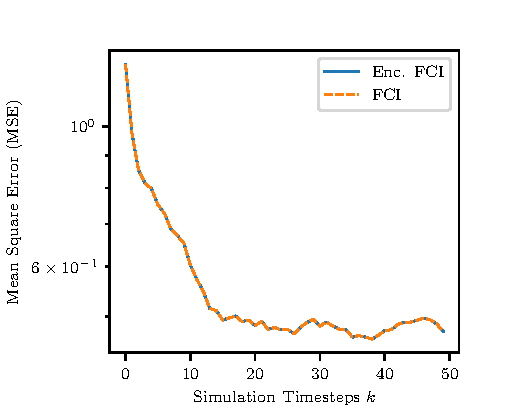
\includegraphics{figures/sim_error_plot.pdf}
    \caption{Average MSE of presented fusion methods over $1000$ simulations.}
    \label{fig:cloud_fusion:secfci2_sim_error}
\end{figure}
From the figure, we can see the expected similarity in performance between all three methods. The better approximation of the fusion weights in the method from this section results in slightly more accurate results than those with the method from section \ref{sec:cloud_fusion:secfci}, however, choosing a smaller stepsize $g$ can reduce this difference, albeit increase complexity.

% 
%  .d8888b.   .d88888b.  888b    888  .d8888b.  
% d88P  Y88b d88P" "Y88b 8888b   888 d88P  Y88b 
% 888    888 888     888 88888b  888 888    888 
% 888        888     888 888Y88b 888 888        
% 888        888     888 888 Y88b888 888        
% 888    888 888     888 888  Y88888 888    888 
% Y88b  d88P Y88b. .d88P 888   Y8888 Y88b  d88P 
%  "Y8888P"   "Y88888P"  888    Y888  "Y8888P"  
%                                               
%                                               
%                                               
% 

\section{Conclusions on Confidential Estimate Fusion}\label{sec:cloud_fusion:conclusion}
In this chapter, we have presented two methods for approximating the FCI fusion algorithm on an untrusted cloud where estimates and final fusion meet specified cryptographic aims. The methods primarily differ in whether the FCI fusion weights are leaked to eavesdroppers and the cloud as well as the assumptions on collusions between parties in the network.

The first method, providing confidential fusion with the leakage of weights, introduced in section \ref{sec:cloud_fusion:secfci}, has the benefit of allowing the untrusted cloud to prioritise sensors when performing fusion. This is done by preferring sensors that reduce fused estimate error, as indicated by their fusion weight, but requires the assumption that sensors are trusted and cannot collude maliciously. The method also requires the use of two encryption schemes, resulting in higher computational complexity at sensors and the cloud, as can be seen in section \ref{subsec:cloud_fusion:secfci_comp_complexity}. The second method, presented in section \ref{sec:cloud_fusion:secfci2}, provides confidential fusion without the leakage of weights. This method doesn't consider sensors as trusted parties and leaks no information beyond the implicit leakage of state dimension, present in both methods. The stronger security guarantees come with disadvantages, namely that the cloud cannot prioritise estimates based on their fusion error and that an additional, albeit constant, complexity is present at the querying party. Both methods have their computational complexity and security implications analysed and are simulated to demonstrate estimation performance.

Future directions for the topic of confidential data fusion include multi-variable encryption, removing the implicit leakage of state dimension, and the extension of the method to decentralised environments where confidential fusion without a centralised cloud is desirable.


\chapter{Distributed Non-Linear Measurement Fusion with Untrusted Participants}\label{ch:nonlin_fusion}

% 
% 8888888b.  8888888b.   .d88888b.  888888b.   
% 888   Y88b 888   Y88b d88P" "Y88b 888  "88b  
% 888    888 888    888 888     888 888  .88P  
% 888   d88P 888   d88P 888     888 8888888K.  
% 8888888P"  8888888P"  888     888 888  "Y88b 
% 888        888 T88b   888     888 888    888 
% 888        888  T88b  Y88b. .d88P 888   d88P 
% 888        888   T88b  "Y88888P"  8888888P"  
%                                              
%                                              
%                                              
% 

\section{Problem Formulation}\label{sec:nonlin_fusion:problem}
This problem aims to lay down a foundation for solving general non-linear measurement fusion where sensor and navigator privacy is preserved and involved data remains confidential. Since solving the general problem is difficult due to broad measurement definitions and the need for concrete communications to be known when proving cryptographic aims, we study a specific non-linear problem instead. The presented solution to this problem then lends itself to solving a class of related, but not exhaustive, non-linear measurement fusion problems with the same communication and cryptographic requirements, discussed later in this chapter. We consider the specific context of confidential range sensor navigation, where no sensor is to learn any information about the navigator or other sensors beyond their local measurements, while the navigator learns no information about individual sensors beyond its location estimate. The problem is two-fold, in that we require explicit cryptographic requirements with a suitable encryption scheme meeting them as well as an estimation scheme that can use the encryption in the context of range-only navigation.

To give a formal cryptographic requirement in a distributed setting, we first consider the communication requirements of our context and define attacker capabilities and the desired security of a suitable encryption scheme. In this section, we define a communication protocol and the relevant formal definition of security we aim to achieve, followed by the estimation problem to which we will apply it.

% 
%  ######  ########  ##    ## ########  ########  #######     ########  ########   #######  ########  
% ##    ## ##     ##  ##  ##  ##     ##    ##    ##     ##    ##     ## ##     ## ##     ## ##     ## 
% ##       ##     ##   ####   ##     ##    ##    ##     ##    ##     ## ##     ## ##     ## ##     ## 
% ##       ########     ##    ########     ##    ##     ##    ########  ########  ##     ## ########  
% ##       ##   ##      ##    ##           ##    ##     ##    ##        ##   ##   ##     ## ##     ## 
% ##    ## ##    ##     ##    ##           ##    ##     ##    ##        ##    ##  ##     ## ##     ## 
%  ######  ##     ##    ##    ##           ##     #######     ##        ##     ##  #######  ########  
% 

\subsection{Formal Cryptographic Problem}\label{subsec:nonlin_fusion:crypto_problem}
The communication between the navigator and sensors in our estimation problem will be decomposed into a simple two-step bi-directional protocol that will simplify defining formal security. In section \ref{subsec:nonlin_fusion:applying_lca_scheme}, we will show how this protocol is sufficient to compute the location estimate at a navigator while meeting our desired privacy goals. The communication protocol is as follows.

At every \textit{instance} $t$ (used to distinguish from an estimation \textit{timestep}), the navigator first broadcasts $l$ weights $\theta_j^{(t)}$, $1\leq j\leq l$, to all sensors $i$, $1\leq i \leq n$, who individually compute linear combinations $e^{(t)}_i=\sum^l_{j=1}a_{j,i}^{(t)}\theta_i^{(t)}$ based on their measurement data $a_{j,i}$. Linear combinations are then sent back to the navigator, who computes their sum $\sum^n_{i=1}e^{(t)}_{i}$. This two-step linear combination aggregation protocol has been visually displayed in figure \ref{fig:nonlin_fusion:aggregation_steps}.
\begin{figure}[htbp]
\centering
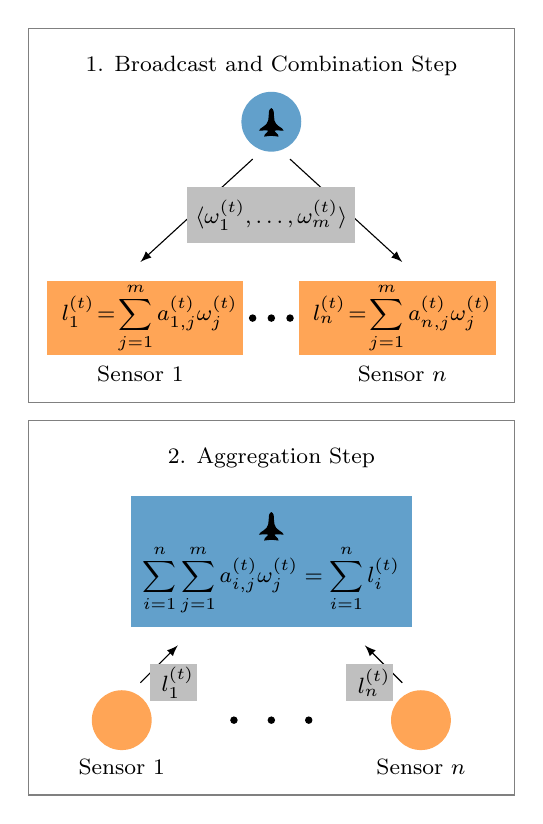
\begin{tikzpicture}[font=\footnotesize,scale=0.95]
    % Step 1
    \node at (3.25,5.5) {1. Broadcast and Combination Step};
    % Navigator
    \fill (3.25,4.75) [pyplotblue!70] ellipse (0.4 and 0.4);
    \pic[xscale=0.22,yscale=0.3] at (3.25,4.9225) {plane};
    % Sensors
    \node at (1.5,1.375) {Sensor $1$};
    \fill [pyplotorange!70] (0.25,1.625) rectangle (2.875,2.625);
    \node at (1.625,2.125) {$\displaystyle l_1^{(t)} \!=\! \sum^m_{j=1}a_{1,j}^{(t)}\omega_j^{(t)}$};
    \node at (5,1.375) {Sensor $n$};
    \fill [pyplotorange!70] (3.625,1.625) rectangle (6.25,2.625);
    \node at (5,2.125) {$\displaystyle l_n^{(t)} \!=\! \sum^m_{j=1}a_{n,j}^{(t)}\omega_j^{(t)}$};
    \fill [black] (3.5,2.125) circle (0.05);
    \fill [black] (3,2.125) circle (0.05);
    \fill [black] (3.25,2.125) circle (0.05);
    % Lines
    \draw [-latex] plot[smooth, tension=.7] coordinates {(3.5,4.25) (5,2.875)};
    \draw [-latex] plot[smooth, tension=.7] coordinates {(3,4.25) (1.5,2.875)};
    \fill [lightgray] (2.125,3.875) rectangle (4.375,3.125);
    \node at (3.25,3.5) {$\langle\omega_1^{(t)},\dots ,\omega_m^{(t)}\rangle$};
    
    % Step 2
    \node at (3.25,0.25) {2. Aggregation Step};
    % Navigator
    \fill [pyplotblue!70] (1.375,-2) rectangle (5.125,-0.25);
    \pic[xscale=0.22,yscale=0.3] at (3.25,-0.4775) {plane};
    \node at (3.25,-1.375) {$\displaystyle \sum^{n}_{i=1}\sum^{m}_{j=1} a_{i,j}^{(t)}\omega_j^{(t)} = \sum^n_{i=1}l^{(t)}_{i}$};
    % Sensors
    \node at (1.25,-3.875) {Sensor $1$};
    \fill  (5.25,-3.25) [pyplotorange!70] ellipse (0.4 and 0.4);
    \node at (5.25,-3.875) {Sensor $n$};
    \fill  (1.25,-3.25) [pyplotorange!70] ellipse (0.4 and 0.4);
    \fill [black] (2.75,-3.25) circle (0.05);
    \fill [black] (3.75,-3.25) circle (0.05);
    \fill [black] (3.25,-3.25) circle (0.05);
    % Lines
    \draw [-latex] plot[smooth, tension=.7] coordinates {(5,-2.75) (4.5,-2.25)};
    \draw [-latex] plot[smooth, tension=.7] coordinates {(1.5,-2.75) (2,-2.25)};
    \fill [lightgray] (1.625,-2.5) rectangle (2.25,-3);
    \node at (2,-2.75) {$l_1^{(t)}$};
    \fill [lightgray] (4.25,-2.5) rectangle (4.875,-3);
    \node at (4.625,-2.75) {$l_n^{(t)}$};
    
    % Bounding rectangles
    \draw [gray] (0,6) rectangle (6.5,1);
    \draw [gray] (0,0.75) rectangle (6.5,-4.25);
\end{tikzpicture}
\caption{Required linear combination aggregation steps at instance $t$.}
\label{fig:nonlin_fusion:aggregation_steps}
% TODO make two subfigures instead. Current text labels should be figure captions. No bounding boxes are required. Update variables as well
\end{figure}
In addition, we note that an alternative approach to the two-step protocol is computing $\sum^{l}_{j=1}(\theta_j^{(t)}\sum^{n}_{i=1} a_{i,j}^{(t)})$ at the navigator, requiring only values $a_{i,j}^{(t)}$, $1\leq j \leq l$, to be sent from each sensor $i$. We justify the use of bi-directional communication by reducing communication costs when the number of weights is larger than the number of sensors, $l>n$, and by sending fewer weights in the presence of repeats, as will be shown to be the case in section \ref{subsec:nonlin_fusion:applying_lca_scheme}.

Before giving a formal definition for the construction and security of our desired encryption scheme, we make the following assumptions about the capabilities of the participants.
\begin{description}
    \item[Global Navigator Broadcast] We assume that broadcast information from the navigator is received by \textit{all} sensors involved in the protocol.
    \item[Consistent Navigator Broadcast] We assume that broadcast information from the navigator is received equally by all sensors. This means the navigator may not send different weights to individual sensors during a single instance $t$.
    \item[Honest-but-Curious Sensors] We adopt the honest-but-curious attacker model for all involved sensors, meaning that they follow the localisation procedure correctly but may store or use any gained sensitive information.
\end{description}
We justify the global broadcast assumption by noting that any subset of sensors within the range of the navigator can be considered a group and treated as the global set during estimation, generalising the method, while the widespread use of cheap non-directional antennas supports the assumption of consistent broadcasts. The final assumption refers to the known problem of misbehaving sensors [lazosSeRLocSecureRangeindependent2004,ben-galOutlierDetection2005], often requiring additional complicated detection mechanisms, and will not be considered in this chapter.

We are now ready to define the type of encryption scheme we want for the specified communication protocol and the security guarantees it should provide. We let a linear combination aggregation scheme be defined as a tuple of the four algorithms $(\mathsf{Setup}, \mathsf{Enc}, \mathsf{CombEnc}, \mathsf{AggDec})$. These will be used by a trusted setup party, the navigator, and sensors $1\leq i\leq n$. They are defined as follows.
\begin{description}
    \item[$\mathsf{Setup}(\kappa)$] On input of security parameter $\kappa$, generate public parameters $\mathsf{pub}$, the number of weights $l$, the navigator's public and private keys $\mathsf{pk}_{\mathsf{a}}$ and $\mathsf{sk}_{\mathsf{a},0}$ and the sensor private keys $\mathsf{sk}_{\mathsf{a},i}$, $1\leq i\leq n$.
    \item[$\mathsf{Enc}(\mathsf{pk}_{\mathsf{a}}, x)$] The navigator and sensors can encrypt any value $x\in\mathbb{Z}$ with the navigator's public key $\mathsf{pk}_{\mathsf{a}}$ and obtain the encryption $\mathcal{E}_{\mathsf{pk}_{\mathsf{a}}}(x)$.
    \item[$\mathsf{CombEnc}(t, \mathsf{pk}_{\mathsf{a}}, \mathsf{sk}_{\mathsf{a},i}, \mathcal{E}_{\mathsf{pk}_{\mathsf{a}}}(\theta_1^{(t)}),\dots,\mathcal{E}_{\mathsf{pk}_{\mathsf{a}}}(\theta_l^{(t)}), a^{(t)}_{i,1},\dots,a^{(t)}_{i,l})$] At instance $t$, sensor $i$ computes and obtains the encrypted linear combination denoted $e^{(t)}_i = \mathcal{E}_{\mathsf{pk}_{\mathsf{a}},\mathsf{sk}_{\mathsf{a},i}}(\sum^l_{j=1}a^{(t)}_{i,j}\theta^{(t)}_j)$ using its secret key $\mathsf{sk}_{\mathsf{a},i}$.
    \item[$\mathsf{AggDec}(t, \mathsf{pk}_{\mathsf{a}}, \mathsf{sk}_{\mathsf{a},0}, e^{(t)}_1,\dots,e^{(t)}_n)$] At instance $t$, the navigator computes the aggregation of linear combinations $\sum^{n}_{i=1}e_i^{(t)}=\sum^{n}_{i=1}\sum^{l}_{j=1} a^{(t)}_{i,j}\theta^{(t)}_j$ using its public and private keys $\mathsf{pk}_{\mathsf{a}}$, $\mathsf{sk}_{\mathsf{a},0}$.
\end{description}
The security notions we want these algorithms to meet reflect the previously stated estimation privacy goals. The navigator should learn no information from individual sensors while sensors should learn no information from the navigator or any other sensors. In the context of the introduced communication protocol, this can be summarised as the following notions.
\begin{description}
    \item[Indistinguishable Weights] No colluding subset of sensors gains any new knowledge about the navigator weights $\theta^{(t)}_j$, $1\leq j\leq l$, when receiving only their encryptions from the current and previous instances and having the ability to encrypt plaintexts of their choice.
    \item[Linear Combination Aggregator Obliviousness] No colluding subset \textit{excluding} the navigator gains additional information about the remaining sensor values to be weighted, $a^{(t)}_{i,j}$, $1\leq j\leq l$, where sensor $i$ is not colluding, given only encryptions of their linear combinations $e_i$ from the current and previous instances. Any colluding subset \textit{including} the navigator learns only the sum of all linear combinations weighted by weights of their choice, $\sum^{n}_{i=1}e_i^{(t)}=\sum^{n}_{i=1}\sum^{l}_{j=1} a^{(t)}_{i,j}\theta^{(t)}_j$.
\end{description}
While indistinguishable weights can be achieved by encrypting weights with an encryption scheme meeting the IND-CPA notion introduced in section \ref{subsec:prelims:crypto_notions}, the novel notion of Linear Combination Aggregator Obliviousness (LCAO) has been formalised as a typical cryptographic game between attacker and challenger in appendix \ref{app:lcao_definition}. Lastly, we conclude the cryptographic problem definition with the following important remark.
\begin{remark}
    A leakage function including weights from the navigator requires extra care to be taken when giving its definition. If an attacker compromises the navigator, they have control over the weights, and therefore the leakage function. We note that in the leakage function above, $\sum^n_{i=1}\sum^l_{j=1}a^{(t)}_{i,j}\theta^{(t)}_j$, an individual sum weighted by the same weight may be learnt by an attacker, \textit{e.g.}, $\sum^n_{i=1}a^{(t)}_{i,1}$ given weights $(1,0,\dots,0)$, but that individual sensor values $a^{(t)}_{i,j}$ remain private due to the assumption of a consistent broadcast.
\end{remark}

% 
% ########  ######  ########    ########  ########   #######  ########  
% ##       ##    ##    ##       ##     ## ##     ## ##     ## ##     ## 
% ##       ##          ##       ##     ## ##     ## ##     ## ##     ## 
% ######    ######     ##       ########  ########  ##     ## ########  
% ##             ##    ##       ##        ##   ##   ##     ## ##     ## 
% ##       ##    ##    ##       ##        ##    ##  ##     ## ##     ## 
% ########  ######     ##       ##        ##     ##  #######  ########  
% 

\subsection{Estimation problem}\label{subsec:nonlin_fusion:estimation_problem}
The estimation problem we consider, for which we will reformulate communication to the protocol above, is localisation with range-only sensors. In this work, we will focus on the two-dimensional case for simplicity but will derive methods suitable for extension to a three-dimensional equivalent. The state that we wish to estimate must capture the navigator position, $x$ and $y$, and may contain any other components relevant to the system. It is of the form
\begin{equation}\label{eq:nonlin_fusion:state_definition}
    \vec{x} = 
    \begin{bmatrix}
        x & y & \cdots
    \end{bmatrix}^\top\,.
\end{equation}
This state evolves following some known system model, which at timestep $k$ can be written as
\begin{equation}\label{eq:nonlin_fusion:system_model}
    \vec{x}_k = \vec{f}_k(\vec{x}_{k-1}, \vec{w}_k)\,,
\end{equation}
with noise term $\vec{w}_k$. Measurements of $\vec{x}_k$ follow a measurement model dependent on sensor $i$, $1\leq i\leq n$, given by 
\begin{equation}\label{eq:nonlin_fusion:measurement_model}
    z_{k,i} = h_i(\vec{x}_k)+v_{k,i}\,,
\end{equation}
with Gaussian measurement noises $v_{k,i} \sim \mathcal{N}(0,r_{k,i})$ and measurement function
\begin{equation}
    \begin{split}
        h_i(\vec{x}) &= \left\lVert
        \begin{bmatrix}
            x & y
        \end{bmatrix}^\top
        - \vec{s}_{i}\right\rVert \\
        &= \sqrt{(x-s_{x,i})^2 + (y-s_{y,i})^2}\,,
    \end{split}
\end{equation}
where
\begin{equation}
    \vec{s}_i = 
    \begin{bmatrix}
        s_{x,i} & s_{y,i}
    \end{bmatrix}^\top
\end{equation} 
is the location of sensor $i$.

We aim to provide a filter that estimates the navigator's state $\vec{x}_k$, at every timestep $k$, without learning sensor positions $\vec{s}_i$, measurements $z_{k, i}$ and measurement variances $r_{k, i}$ beyond the information in the corresponding aggregation leakage function. Similarly, sensors should not learn any information about current state estimates or any other sensor information. Leakage will be further discussed in section \ref{subsec:nonlin_fusion:security}, but we note that from any sequential state estimates, following known models, some sensor information leakage can be computed by the navigator. In the context of our leakage function, we will show that this corresponds to the global sums of private sensor information, while individual, or subsets of sensors', information remains private. Similarly, corrupted sensors with access to one or more measurements can produce state estimates of their own, leaking information about navigator state estimates, however, the most accurate estimates, requiring all measurements, will always remain private to the navigator.

% 
% 888      .d8888b.        d8888 
% 888     d88P  Y88b      d88888 
% 888     888    888     d88P888 
% 888     888           d88P 888 
% 888     888          d88P  888 
% 888     888    888  d88P   888 
% 888     Y88b  d88P d8888888888 
% 88888888 "Y8888P" d88P     888 
%                                
%                                
%                                
% 

\section{A Linear Combination Aggregation Scheme}\label{sec:nonlin_fusion:lcao_scheme}
In this section, we introduce an encryption scheme meeting the desired security properties in section \ref{subsec:nonlin_fusion:crypto_problem}. The scheme is a combination of the Paillier and Joye-Libert schemes, introduced in section \ref{subsec:prelims:paillier} and \ref{subsec:prelims:joye_libert_agg}, respectively, that provides encrypted weights meeting the IND-CPA notion and encrypted aggregation meeting the LCAO notion in appendix \ref{app:lcao_definition}. Similarly to its constituents, the scheme bases its security on the DCRA and, as with the Joye-Libert scheme, requires a trusted party for initial key generation and distribution. 

As aggregation is typically performed on scalar inputs, we extend our notation to the context of multidimensional estimation data by letting an instance $t_{k,\epsilon}$ uniquely capture the scalar aggregation during an estimation timestep $k$ for a single element with position index $\epsilon$. To achieve this in practice, any injective function can be used, such as the concatenation $t_{k,\epsilon}=k\mathbin\|\epsilon$. The four algorithms defining our scheme are given as follows.
\begin{description}
    \item[$\mathsf{Setup}(\kappa)$] On input parameter $\kappa$, generate two equal-length, sufficiently large, primes $p$ and $q$, and compute $N=pq$. Define a hash function $H:\mathbb{Z} \rightarrow \mathbb{Z}_{N^2}^*$, choose the number of weights to combine, $l>1$, and set public parameter $\mathsf{pub}=H$, navigator public key $\mathsf{pk}_{\mathsf{a}} = N$ and navigator private key $\mathsf{sk}_{\mathsf{a},0}=(p,q)$. Sensor secret keys are generated by choosing $\mathsf{sk}_{\mathsf{a},i}$, $1\leq i\leq n-1$, uniformly from $\mathbb{Z}_{N^2}$ and setting the last key to $\mathsf{sk}_{\mathsf{a},n} = -\sum^{n-1}_{i=1}\mathsf{sk}_{\mathsf{a},i}$.
 
    \item[$\mathsf{Enc}(\mathsf{pk}_{\mathsf{a}}, x)$] Public-key encryption is computed by the Paillier encryption scheme in section \ref{subsec:prelims:paillier}. This is given by
    \begin{equation}\label{eq:nonlin_fusion:lca_scheme_encryption}
        \mathcal{E}_{\mathsf{pk}_{\mathsf{a}}}(x) = (N+1)^{x}\rho^N \pmod{N^2}\,,
    \end{equation}
    for a randomly chosen $\rho \in \mathbb{Z}_N$.

    \item[$\mathsf{CombEnc}(t_{k,\epsilon}, \mathsf{pk}_{\mathsf{a}}, \mathsf{sk}_{\mathsf{a},i}, \mathcal{E}_{\mathsf{pk}_{\mathsf{a}}}(\theta_1^{(k,\epsilon)}),\dots,\mathcal{E}_{\mathsf{pk}_{\mathsf{a}}}(\theta_l^{(k,\epsilon)}), a^{(k,\epsilon)}_{i,1},\dots,a^{(k,\epsilon)}_{i,l})$] At the instance $t_{k,\epsilon}$, encrypted linear combination is given by 
    \begin{equation}\label{eq:nonlin_fusion:lca_scheme_lin_comb}
        e^{(k,\epsilon)}_i = H(t_{k,\epsilon})^{\mathsf{sk}_{\mathsf{a},i}}\prod^{l}_{j=1}\mathcal{E}_{\mathsf{pk}_{\mathsf{a}}}(\theta^{(k,\epsilon)}_j)^{a^{(k,\epsilon)}_{i,j}} \pmod{N^2}\,,
    \end{equation}
    making use of the Paillier homomorphic properties \eqref{eq:prelims:paillier_hom_add} and \eqref{eq:prelims:paillier_hom_mult}. Correctness follows from
    \begin{equation*}
        \begin{split}
            e^{(k,\epsilon)}_i &= H(t_{k,\epsilon})^{\mathsf{sk}_{\mathsf{a},i}}\prod^{l}_{j=1}\mathcal{E}_{\mathsf{pk}_{\mathsf{a}}}(\theta^{(k,\epsilon)}_j)^{a^{(k,\epsilon)}_{i,j}} \pmod{N^2} \\
            &= H(t_{k,\epsilon})^{\mathsf{sk}_{\mathsf{a},i}}\prod^{l}_{j=1}\mathcal{E}_{\mathsf{pk}_{\mathsf{a}}}(a^{(k,\epsilon)}_{i,j}\theta^{(k,\epsilon)}_j) \pmod{N^2} \\
            &= H(t_{k,\epsilon})^{\mathsf{sk}_{\mathsf{a},i}}\prod^{l}_{j=1}(N+1)^{a^{(k,\epsilon)}_{i,j}\theta^{(k,\epsilon)}_j} \rho^{N}_{j} \pmod{N^2} \\
            &= H(t_{k,\epsilon})^{\mathsf{sk}_{\mathsf{a},i}}(N+1)^{\sum^{l}_{j=1}a^{(k,\epsilon)}_{i,j}\theta^{(k,\epsilon)}_j} \tilde{\rho}_{i}^{N} \pmod{N^2}\,,
        \end{split}
    \end{equation*}
    for some values $\rho_j \in \mathbb{Z}_N$, $1\leq j\leq l$, and $\tilde{\rho}_i=\prod^{l}_{j=1}\rho_j$. Here, $\tilde{\rho}_i^N$ and $H(t_{k,\epsilon})^{\mathsf{sk}_{\mathsf{a}, i}}$ can be considered the noise terms corresponding to the two levels of encryption from $\mathsf{pk}_{\mathsf{a}}$ and $\mathsf{sk}_{\mathsf{a}, i}$, respectively.

    \item[$\mathsf{AggDec}(t_{k,\epsilon}, \mathsf{pk}_{\mathsf{a}}, \mathsf{sk}_{\mathsf{a},0}, e^{(k,\epsilon)}_1,\dots,e^{(k,\epsilon)}_n)$] Aggregation is computed as $e^{(k,\epsilon)} = \prod^n_{i=1}e^{(k,\epsilon)}_i\pmod{N^2}$, removing the aggregation noise terms, and is followed by Paillier scheme decryption
    \begin{equation}\label{eq:nonlin_fusion:lca_scheme_decryption}
        \sum^{n}_{i=1}\sum^{l}_{j=1} a^{(k,\epsilon)}_{i,j}\theta^{(k,\epsilon)}_j = \frac{L((e^{(k,\epsilon)})^\lambda\pmod{N^2})}{L((N+1)^\lambda\pmod{N^2})} \pmod{N}\,,
    \end{equation}
    with $\lambda = \mathsf{lcm}(p-1, q-1)$ and $L(\psi) = \frac{\psi-1}{N}$. The correctness of the aggregation can be seen from
    \begin{align*}
        e^{(k,\epsilon)} &= \prod^n_{i=1}H(t_{k,\epsilon})^{\mathsf{sk}_{\mathsf{a},i}}(N+1)^{\sum^{l}_{j=1}a^{(k,\epsilon)}_{i,j}\theta^{(k,\epsilon)}_j}\tilde{\rho}_i^N \pmod{N^2}\\
        &= H(t_{k,\epsilon})^{\sum^n_{i=1}\mathsf{sk}_{\mathsf{a},i}}\prod^n_{i=1}(N+1)^{\sum^{l}_{j=1}a^{(k,\epsilon)}_{i,j}\theta^{(k,\epsilon)}_j}\tilde{\rho}_i^N \pmod{N^2}\\
        &= (N+1)^{\sum^n_{i=1}\sum^{l}_{j=1}a^{(k,\epsilon)}_{i,j}\theta^{(k,\epsilon)}_j}\tilde{\rho}^N\pmod{N^2}\,,
    \end{align*}
    for some values $\tilde{\rho}_i \in \mathbb{Z}_N$, $1\leq i\leq n$, and $\tilde{\rho}=\prod^{n}_{i=1}\tilde{\rho}_i$.
\end{description}
Additionally, we note that in the above construction, all weights $\theta^{(k,\epsilon)}_j$ and values $a^{(k,\tau)}_{i,j}$ are integers and the resulting linear combinations and aggregation are computed modulo $N$. 

The security proof of this scheme must both show that encrypted weights meet IND-CPA and that encrypted aggregation meets LCAO. As weights are encrypted with the Paillier encryption scheme, the first requirement is already met. To show that aggregation meets LCAO, a reduction proof is given in appendix \ref{app:lca_scheme_proof}.

\begin{remark}
    Given the construction of the scheme above, it can be seen that any weights $\theta^{(k,\epsilon)}_j$, whose values are known at each sensor, do not need to be broadcast by the navigator. In this case, sensors can replace
    \begin{equation}
        \mathcal{E}_{\mathsf{pk}_{\mathsf{a}}}(\theta^{(k,\epsilon)}_j)^{a^{(k,\epsilon)}_{i,j}} = (N+1)^{\theta^{(k,\epsilon)}_j a^{(k,\epsilon)}_{i,j}}\rho_j^N \pmod{N^2}
    \end{equation}
    in \eqref{eq:nonlin_fusion:lca_scheme_lin_comb}, by
    \begin{equation}
        (N+1)^{\theta^{(k,\epsilon)}_j a^{(k,\epsilon)}_{i,j}} \pmod{N^2}\,.
    \end{equation}
    This is due to the removal of $\rho_j^N$ terms during decryption and can be used to reduce the navigator's broadcast communication cost by the number of weights $\theta^{(k,\epsilon)}_j$ that do not hold any information private to the navigator and are known by the sensors in advance.
\end{remark}

% 
% 8888888b.         d8888 888b    888  .d8888b.  8888888888      888      .d88888b.   .d8888b.  
% 888   Y88b       d88888 8888b   888 d88P  Y88b 888             888     d88P" "Y88b d88P  Y88b 
% 888    888      d88P888 88888b  888 888    888 888             888     888     888 888    888 
% 888   d88P     d88P 888 888Y88b 888 888        8888888         888     888     888 888        
% 8888888P"     d88P  888 888 Y88b888 888  88888 888             888     888     888 888        
% 888 T88b     d88P   888 888  Y88888 888    888 888             888     888     888 888    888 
% 888  T88b   d8888888888 888   Y8888 Y88b  d88P 888             888     Y88b. .d88P Y88b  d88P 
% 888   T88b d88P     888 888    Y888  "Y8888P88 8888888888      88888888 "Y88888P"   "Y8888P"  
%                                                                                               
%                                                                                               
%                                                                                               
% 

\section{Confidential Range-Only Localisation}\label{sec:nonlin_fusion:conf_range_only_localisation}
With a concrete scheme meeting the LCAO notion, we now put forward a localisation filter with communication that can be reformulated to the required protocol. To produce an estimate of the state $\vec{x}_k$, we make use of the EKF, introduced in section \ref{subsec:prelims:ekf}. The EKF is performed on the information form of the state estimate and its error covariance, repeated here for convenience. That is, the information vector and information matrix,
\begin{equation}\label{eq:nonlin_fusion:eif_info_vec_info_mat}
    \hat{\vec{y}}_{k|k-1} = \mat{P}_{k|k-1}^{-1}\hat{\vec{x}}_{k|k-1} \text{ and } \mat{Y}_{k|k-1} = \mat{P}_{k|k-1}^{-1}\,,
\end{equation}
respectively. In this form, the update equations for $n$ sensor measurements at time $k$, with measurement models \eqref{eq:nonlin_fusion:measurement_model}, are given by
\begin{equation}\label{eq:nonlin_fusion:eif_info_vec_update}
        \hat{\vec{y}}_{k|k} = \hat{\vec{y}}_{k|k-1} +  \sum^n_{i=1}\mat{H}^\top_{k,i} r^{-1}_i \left(z_{k,i} - h_i(\hat{\vec{x}}_{k|k-1}) + \mat{H}_{k,i}\hat{\vec{x}}_{k|k-1}\right)
\end{equation}
and
\begin{equation}\label{eq:nonlin_fusion:eif_info_mat_update}
    \mat{Y}_{k|k} = \mat{Y}_{k|k-1} + \sum^n_{i=1}\mat{H}^\top_{k,i} r^{-1}_i \mat{H}_{k,i}\,,
\end{equation}
with Jacobians
\begin{equation}\label{eq:nonlin_fusion:measurement_jacobian}
    \mat{H}_{k,i} = \left.\frac{\partial h_i}{\partial \vec{x}}\right|_{\hat{\vec{x}}_{k|k-1}}
\end{equation}
for sensors $1\leq i\leq n$. The updated information vector and matrix can then be used in a local filter prediction step at the navigator, using any suitable filter for the known system model \eqref{eq:nonlin_fusion:system_model}.

In the form above, at every timestep $k$, all sensitive sensor information required for state estimation is captured in the measurement vector
\begin{equation}\label{eq:nonlin_fusion:measurement_vec}
    \vec{i}_{k,i} = \mat{H}^\top_{k,i} r^{-1}_i \left(z_{k,i} - h_i(\hat{\vec{x}}_{k|k-1}) + \mat{H}_{k,i}\hat{\vec{x}}_{k|k-1}\right)
\end{equation}
and the measurement matrix
\begin{equation}\label{eq:nonlin_fusion:measurement_mat}
    \mat{I}_{k,i} = \mat{H}^\top_{k,i} r^{-1}_i \mat{H}_{k,i}\,,
\end{equation}
namely, their measurements $z_{k,i}$, measurement variances $r_{k,i}$ and locations $\vec{s}_i$; captured in measurement functions $h_i$ and Jacobians $\mat{H}_{k,i}$. However, computing $\vec{i}_{k,i}$ and $\mat{I}_{k,i}$ also requires the current predicted state estimate $\hat{\vec{x}}_{k|k-1}$, when evaluating $h_i$ and $\mat{H}_{k,i}$. To achieve the communication protocol desired, we aim to rearrange \eqref{eq:nonlin_fusion:measurement_vec} and \eqref{eq:nonlin_fusion:measurement_mat} as a linear combination of functions of $\hat{\vec{x}}_{k|k-1}$ (considered the navigator weights), computable at each sensor $i$, to be subsequently aggregated at the navigator. Application of the linear combination aggregation scheme proposed can then guarantee that sensors do not learn the navigator state, and the navigator learns only the aggregation required for updating its estimate \eqref{eq:nonlin_fusion:eif_info_vec_update} and \eqref{eq:nonlin_fusion:eif_info_mat_update}.

% 
% ########     ###    ##    ##  ######   ########    ##     ##  #######  ########  
% ##     ##   ## ##   ###   ## ##    ##  ##          ###   ### ##     ## ##     ## 
% ##     ##  ##   ##  ####  ## ##        ##          #### #### ##     ## ##     ## 
% ########  ##     ## ## ## ## ##   #### ######      ## ### ## ##     ## ##     ## 
% ##   ##   ######### ##  #### ##    ##  ##          ##     ## ##     ## ##     ## 
% ##    ##  ##     ## ##   ### ##    ##  ##          ##     ## ##     ## ##     ## 
% ##     ## ##     ## ##    ##  ######   ########    ##     ##  #######  ########  
% 

\subsection{Range Measurement Modification}\label{subsec:nonlin_fusion:measurement_modification}
Rearranging $\vec{i}_{k, i}$ and $\mat{I}_{k, i}$ to a linear combination of functions of $\hat{\vec{x}}_{k|k-1}$, we note that $h_i$ does not inherently support this due to the present square-root. Similarly, the Jacobian of $h_i$ at $\hat{\vec{x}}_{k|k-1}$,
\begin{equation}
    \mat{H}_{k,i} = 
    \begin{bmatrix}
        \frac{\hat{x}_{k|k-1} - s_{x,i}}{\sqrt{(\hat{x}_{k|k-1} - s_{x,i})^2 + (\hat{y}_{k|k-1} - s_{y,i})^2}} \\
        \frac{\hat{y}_{k|k-1} - s_{y,i}}{\sqrt{(\hat{x}_{k|k-1} - s_{x,i})^2 + (\hat{y}_{k|k-1} - s_{y,i})^2}} \\
        0 \\
        \vdots
    \end{bmatrix}^\top\,,
\end{equation}
does not either. Instead, the modified measurement functions
\begin{equation}\label{eq:nonlin_fusion:modified_measurement_func}
    h'_i(\vec{x}) = h_i(\vec{x})^2\,,
\end{equation}
are considered. In this form, the functions allow rearrangement of $h'_i$ and the corresponding Jacobian $\mat{H}'_{k,i}$ to a linear combination of powers of location elements in $\hat{\vec{x}}_{k|k-1}$, as
\begin{equation}
    \begin{split}
        h'_i(\vec{x}) &= \left\lVert
        \begin{bmatrix}
            x & y
        \end{bmatrix}^\top - \vec{s}_i\right\rVert^2 \\
        &= (x - s_{x,i})^2 + (y - s_{y,i})^2 \\
        &= x^2 + y^2 -2s_{x,i}x -2s_{y,i}y +s_{x,i}^2 +s_{y,i}^2\,,
    \end{split}
\end{equation}
and
\begin{equation}\label{eq:nonlin_fusion:modified_jacobian}
    \mat{H}'_{k,i} = 
    \begin{bmatrix}
        2\hat{x}_{k|k-1} - 2s_{x,i} \\
        2\hat{y}_{k|k-1} - 2s_{y,i} \\
        0 \\
        \vdots
    \end{bmatrix}^\top\,.
\end{equation}
Here, $h'_i$ and $\mat{H}'_{k,i}$ are linear combinations of $\hat{x}_{k|k-1}^2$, $\hat{y}_{k|k-1}^2$, $\hat{x}_{k|k-1}$ and $\hat{y}_{k|k-1}$. For the rearrangement of corresponding modified measurement vectors $\vec{i}'_{k, i}$ and matrices $\mat{I}'_{k, i}$, usable for the desired localisation update, we also require the existence of measurements following the considered modified measurement models,
\begin{equation}\label{eq:nonlin_fusion:modified_measurement_model}
    z'_{k,i} = h'_i(\vec{x}_k)+v'_{k,i}\,,
\end{equation}
where $z'_{k,i}$ is the modified measurement, and noise term $v'_{k,i}$ is zero-mean and has a known variance $r'_{k,i}$.

Computing $z'_{k,i}$ and its variance $r'_{k,i}$ from the original measurements $z_{k,i}$ is complicated by the original noise term $v_{k,i} \sim \mathcal{N}(0, r_{k,i})$. Squaring the original range measurements produces
\begin{equation}
    \begin{split}
        z_{k,i}^2 &= (h_i(\vec{x}_k) + v_{k,i})^2 \\
        &= h'_i(\vec{x}_k) + 2h_i(\vec{x}_k)v_{k,i} + v_{k,i}^2\,,
    \end{split}
\end{equation}
with a new noise term $2h_i(\vec{x}_k)v_{k,i} + v_{k,i}^2$, now dependent on the measurement function $h_i$, and no longer zero-mean. The mean of this new noise term (a function of the Gaussian term $v_{k, i}$) is given by $\mathsf{E}[2h_i(\vec{x}_k)v_{k, i} + v_{k, i}^2] = r_{k, i}$ and can be used to mean-adjust the squared measurement above, producing the modified measurements
\begin{equation}\label{eq:nonlin_fusion:modified_measurement}
    \begin{split}
        z'_{k,i} &= z_{k,i}^2 - r_{k,i} \\
        &= h_i(\vec{x}_k)^2 + 2h_i(\vec{x}_k)v_{k,i} + v_{k,i}^2 - r_{k,i} \\
        &= h'_i(\vec{x}_k) + v'_{k,i}\,,
    \end{split}
\end{equation}
with now zero-mean noise term $v'_{k,i} = 2h_i(\vec{x}_k)v_{k,i} + v_{k,i}^2 - r_{k,i}$. This noise, again a function of $v_{k,i}$, has variance 
\begin{equation}\label{eq:nonlin_fusion:modified_measurement_variance}
    \mathsf{Var}[v'_{k,i}] = 4h_i(\vec{x}_k)^2r_{k,i} + 2r_{k,i}^2\,,
\end{equation}
still dependent on $h_i$. To use the modified measurements \eqref{eq:nonlin_fusion:modified_measurement} with the EIF, we require an estimate for $\mathsf{Var}[v'_{k, i}]$ at the sensor as well. Additionally, a conservative estimate, that is, a larger variance resulting in less confidence in measurements, is desirable to reduce filter divergence. Intuitively replacing $h_i(\vec{x}_k)$ with $z_{k, i}$ in \eqref{eq:nonlin_fusion:modified_measurement_variance} may not provide a conservative estimate when $z_{k, i}^2 < h_i(\vec{x}_k)^2$, but Gaussianity of $v_{k, i}$ and the squaring of $z_{k, i}$ can be exploited to provide a conservative estimate, with $95\%$ confidence, by adding two of its standard deviations, $\sqrt{r_{k, i}}$, to the replacement term $z_{k, i}$. The modified measurement's variance at timestep $k$ is then conservatively approximated by
\begin{equation}\label{eq:nonlin_fusion:modified_measurement_variance_estimate}
    \begin{split}
        r'_{k, i} &= 4(z_{k,i} + 2\sqrt{r_{k,i}})^2r_{k,i} + 2r_{k,i}^2 \\
        &\gtrapprox \mathsf{Var}[v'_{k,i}]\,,
    \end{split}
\end{equation}
at each sensor $i$.

The modified measurement model \eqref{eq:nonlin_fusion:modified_measurement_model} can now be used for localisation, when measurements are modified by \eqref{eq:nonlin_fusion:modified_measurement} and their new variances estimated with \eqref{eq:nonlin_fusion:modified_measurement_variance_estimate}.

% 
% ##     ##  ######  #### ##    ##  ######      ##        ######     ###    
% ##     ## ##    ##  ##  ###   ## ##    ##     ##       ##    ##   ## ##   
% ##     ## ##        ##  ####  ## ##           ##       ##        ##   ##  
% ##     ##  ######   ##  ## ## ## ##   ####    ##       ##       ##     ## 
% ##     ##       ##  ##  ##  #### ##    ##     ##       ##       ######### 
% ##     ## ##    ##  ##  ##   ### ##    ##     ##       ##    ## ##     ## 
%  #######   ######  #### ##    ##  ######      ########  ######  ##     ## 
% 

\subsection{Applying the Linear Combination Aggregation Scheme}\label{subsec:nonlin_fusion:applying_lca_scheme}
To complete the EIF update as a linear combination aggregation, modified vectors $\vec{i}'_{k, i}$ and matrices $\mat{I}'_{k, i}$, using the modified measurement model \eqref{eq:nonlin_fusion:modified_measurement_model}, can be rearranged as
\begin{equation}\label{eq:nonlin_fusion:hrz_linear_comb}
    \begin{split}
        \vec{i}'_{k,i} &= \mat{H}_{k,i}^{\prime\top} r_{k,i}^{\prime-1}(z'_{k,i} - h'_i(\hat{\vec{x}}_{k|k-1}) + \mat{H}'_{k,i}\hat{\vec{x}}_{k|k-1}) \\
        &= 
        \begin{bmatrix}
            \alpha_i^{(k,1)} & \alpha_i^{(k,2)} & 0 & \cdots
        \end{bmatrix}^\top\,,
    \end{split}
\end{equation}
with
\begin{align*}
    \begin{split}
        \alpha_i^{(k,1)} &= (2r_{k,i}^{\prime-1})\hat{x}_{k|k-1}^3 + (2r_{k,i}^{\prime-1})\hat{x}_{k|k-1}\hat{y}_{k|k-1}^2+ (-2r_{k,i}^{\prime-1}s_{x,i})\hat{x}_{k|k-1}^2 + (-2r_{k,i}^{\prime-1}s_{x,i})\hat{y}_{k|k-1}^2 \\
        &\quad+ (2r_{k,i}^{\prime-1}z'_{k,i})\hat{x}_{k|k-1} + (-2r_{k,i}^{\prime-1}s_{x,i}^2)\hat{x}_{k|k-1}+ (-2r_{k,i}^{\prime-1}s_{y,i}^2)\hat{x}_{k|k-1} + (2r_{k,i}^{\prime-1}s_{x,i}^3) \\
        &\quad+ (2r_{k,i}^{\prime-1}s_{x,i}s_{y,i}^2) + (-2r_{k,i}^{\prime-1}s_{x,i} z'_{k,i})\,,
    \end{split}\\
    \begin{split}
        \alpha_i^{(k,2)} &= (2r_{k,i}^{\prime-1})\hat{y}_{k|k-1}^3 + (2r_{k,i}^{\prime-1})\hat{x}_{k|k-1}^2\hat{y}_{k|k-1}+ (-2r_{k,i}^{\prime-1}s_{y,i})\hat{x}_{k|k-1}^2 + (-2r_{k,i}^{\prime-1}s_{y,i})\hat{y}_{k|k-1}^2 \\
        &\quad+ (2r_{k,i}^{\prime-1}z'_{k,i})\hat{y}_{k|k-1} + (-2r_{k,i}^{\prime-1}s_{x,i}^2)\hat{y}_{k|k-1}+ (-2r_{k,i}^{\prime-1}s_{y,i}^2)\hat{y}_{k|k-1} + (2r_{k,i}^{\prime-1}s_{y,i}s_{x,i}^2) \\
        &\quad+ (2r_{k,i}^{\prime-1}s_{y,i}^3) + (-2r_{k,i}^{\prime-1}s_{y,i}z'_{k,i})\,,
    \end{split}
\end{align*}
and
\begin{equation}\label{eq:nonlin_fusion:hrh_linear_comb}
    \begin{split}
        \mat{I}'_{k,i} &= \mat{H}_{k,i}^{\prime\top} r_{k,i}^{\prime-1}\mat{H}'_{k,i} \\
        &=
        \begin{bmatrix}
            \alpha_i^{(k,3)} & \alpha_i^{(k,4)} & 0 & \cdots \\
            \alpha_i^{(k,5)} & \alpha_i^{(k,6)} & 0 & \cdots\\
            0 & 0 & 0 & \cdots \\
            \vdots & \vdots & \vdots & \ddots
        \end{bmatrix}\,,
    \end{split}
\end{equation}
with
\begin{align*}
    \alpha_i^{(k,3)} &= (4r_{k,i}^{\prime-1})\hat{x}_{k|k-1}^2 + (-8r_{k,i}^{\prime-1}s_{x,i})\hat{x}_{k|k-1} + (4r_{k,i}^{\prime-1}s_{x,i}^2)\,,\\
    \alpha_i^{(k,4)} &= (4r_{k,i}^{\prime-1})\hat{x}_{k|k-1}\hat{y}_{k|k-1} + (-4r_{k,i}^{\prime-1}s_{y,i})\hat{x}_{k|k-1} + (-4r_{k,i}^{\prime-1}s_{x,i})\hat{y}_{k|k-1} + (4r_{k,i}^{\prime-1}s_{x,i}s_{y,i})\,,\\
    \alpha_i^{(k,5)} &= \alpha_i^{(k,4)}\,,\\
    \alpha_i^{(k,6)} &= (4r_{k,i}^{\prime-1})\hat{y}_{k|k-1}^2 + (-8r_{k,i}^{\prime-1}s_{y,i})\hat{y}_{k|k-1} + (4r_{k,i}^{\prime-1}s_{y,i}^2)\,.
\end{align*}
The above rearrangements give $\vec{i}'_{k,i}$ and $\mat{I}'_{k,i}$ as linear combinations of elements in
\begin{equation}\label{eq:nonlin_fusion:weights_to_broadcast}
    \begin{split}
        &\{ \hat{x}_{k|k-1}^3,\ \hat{y}_{k|k-1}^3,\ \hat{x}_{k|k-1}^2\hat{y}_{k|k-1},\ \hat{x}_{k|k-1}\hat{y}_{k|k-1}^2,\\
        &\quad \hat{x}_{k|k-1}^2,\ \hat{y}_{k|k-1}^2,\ \hat{x}_{k|k-1}\hat{y}_{k|k-1},\ \hat{x}_{k|k-1},\ \hat{y}_{k|k-1}\}\,,
    \end{split}
\end{equation}
that capture all private state information in $\hat{\vec{x}}_{k|k-1}$ required by the sensors. The corresponding EIF update steps \eqref{eq:nonlin_fusion:eif_info_vec_update} and \eqref{eq:nonlin_fusion:eif_info_mat_update} then become
\begin{equation}\label{eq:nonlin_fusion:eif_modified_vec_update}
    \hat{\vec{y}}_{k|k} = \hat{\vec{y}}_{k|k-1} + \sum^n_{i=1}\vec{i}'_{k,i}
\end{equation}
and
\begin{equation}\label{eq:nonlin_fusion:eif_modified_mat_update}
    \mat{Y}_{k|k} = \mat{Y}_{k|k-1} + \sum^n_{i=1}\mat{I}'_{k,i}\,,
\end{equation}
respectively.
\begin{remark}
    The above has been derived for two-dimensional localisation but can be similarly derived for the three-dimensional case. However, as can be seen from the rearrangements, the number of weights increases combinatorially with the state dimension, thus affecting the cost of communication as well.
\end{remark}

% 
%    ###    ##        ######    ######  
%   ## ##   ##       ##    ##  ##    ## 
%  ##   ##  ##       ##        ##       
% ##     ## ##       ##   ####  ######  
% ######### ##       ##    ##        ## 
% ##     ## ##       ##    ##  ##    ## 
% ##     ## ########  ######    ######  
% 

\subsection{Pseudocode}\label{subsec:nonlin_fusion:pseudocode}
Measurement modification, number encoding and linear combination aggregation are all required to compute the EIF from the previous section and keep all sensor and navigator information confidential. In this section, we summarise this process and give the pseudocode for its execution. As in the previous chapter, we use the  Q number format in section \ref{subsec:prelims:encoding} for encoding real number inputs, letting $M=N$, where $N$ is the generated public key, choose an appropriate precision $\phi$ and denote encoding with $\delta$ previous multiplications as $\mathsf{E}_{\delta}(\cdot)$. The confidential localisation filter consists of the following steps.
\begin{description}
    \item[Setup] The $\mathsf{Setup}$ algorithm from section \ref{sec:nonlin_fusion:lcao_scheme} is run only once by a trusted party. $\mathsf{pub}=H$ and the navigator public key $\mathsf{pk}_{\mathsf{a}}=N$ are made public, and the navigator and sensor secret keys, $\mathsf{sk}_{\mathsf{a},0}=(p, q)$ and $\mathsf{sk}_{\mathsf{a}, i}$, $1\leq i\leq n$, are distributed accordingly.

    \item[Prediction] At each timestep $k$, the navigator computes the prediction of the current state and its covariance with a local filter before encrypting weights \eqref{eq:nonlin_fusion:weights_to_broadcast} with $\mathsf{Enc}$ and broadcasting them to the sensors. This has been shown in algorithm \ref{alg:nonlin_fusion:nav_prediction}.

    \item[Measurement] At each timestep $k$, sensors modify their measurements with \eqref{eq:nonlin_fusion:modified_measurement} and \eqref{eq:nonlin_fusion:modified_measurement_variance_estimate} before computing elementwise encryptions of $\vec{i}'_{k, i}$ and $\mat{I}'_{k, i}$ with $\mathsf{CombEnc}$ and sending them back to the navigator. This is shown in algorithm \ref{alg:nonlin_fusion:sen_measurement}.

    \item[Update] At each timestep $k$, the navigator aggregates and decrypts received measurement vectors and matrices with $\mathsf{AggDec}$, before computing the EIF update equations \eqref{eq:nonlin_fusion:eif_modified_vec_update} and \eqref{eq:nonlin_fusion:eif_modified_mat_update}. This is shown in algorithm \ref{alg:nonlin_fusion:nav_update}.
\end{description}

\begin{algorithm}[htbp]
\caption{Navigator Prediction}\label{alg:nonlin_fusion:nav_prediction}
\begin{algorithmic}[1]
    \setstretch{1.35}
    \Procedure{Prediction}{$\hat{\vec{y}}_{k-1|k-1}$, $\mat{Y}_{k-1|k-1}$, $\mathsf{pk}_{\mathsf{a}}$}
    \LineComment{Compute local prediction}
    \State Estimate $\hat{\vec{y}}_{k|k-1}$ locally
    \State Estimate $\mat{Y}_{k|k-1}$ locally

    \LineComment{Encode, encrypt and broadcast weights}
    \State Compute $\mathcal{E}_{\mathsf{pk}_{\mathsf{a}}}\left(\mathsf{E}_{0}\left(\hat{x}^3_{k|k-1}\right)\right)$ given \eqref{eq:nonlin_fusion:eif_info_vec_info_mat}
    \State Broadcast $\mathcal{E}_{\mathsf{pk}_{\mathsf{a}}}\left(\mathsf{E}_{0}\left(\hat{x}^3_{k|k-1}\right)\right)$ to sensors
    \For{Remaining weights in \eqref{eq:nonlin_fusion:weights_to_broadcast}} 
        \State Encode, encrypt and broadcast weight in the form above
    \EndFor

    \State \Return $\hat{\vec{y}}_{k|k-1}, \mat{Y}_{k|k-1}$
    \EndProcedure
\end{algorithmic}
\end{algorithm}

\begin{algorithm}[htbp]
\caption{Measurement at Sensor $i$}\label{alg:nonlin_fusion:sen_measurement}
\begin{algorithmic}[1]
    \setstretch{1.35}
    \Procedure{Measurement}{$i$, $s_{x,i}$, $s_{y,i}$, $r_{k,i}$, $\mathsf{pub}$, $\mathsf{pk}_{\mathsf{a}}$, $\mathsf{sk}_{\mathsf{a},i}$}
    \State $H \gets \mathsf{pub}$
    \State $N \gets \mathsf{pk}_{\mathsf{a}}$

    \LineComment{Measure and modify measurement}
    \State Measure $z_{k,i}$
    \State Compute $z'_{k,i}$ by \eqref{eq:nonlin_fusion:modified_measurement}
    \State Compute $r'_{k,i}$ by \eqref{eq:nonlin_fusion:modified_measurement_variance_estimate}

    \LineComment{Receive encrypted weights}
    \State Recieve $\mathcal{E}_{\mathsf{pk}_{\mathsf{a}}}\left(\mathsf{E}_{0}\left(\hat{x}^3_{k|k-1}\right)\right)$
    \For{Remaining weights in \eqref{eq:nonlin_fusion:weights_to_broadcast}}
        \State Recieve weight in the form above
    \EndFor

    \LineComment{Compute linear combination of measurement vector and matrix components}
    \State Let $\bm{\alpha}_{i}^{(k,\epsilon)}$ represent the encryption of $\alpha_{i}^{(k,\epsilon)}$ in \eqref{eq:nonlin_fusion:hrz_linear_comb} and \eqref{eq:nonlin_fusion:hrh_linear_comb}
    \State $\bm{\alpha}_{i}^{(k,1)} \gets \mathcal{E}_{\mathsf{pk}_{\mathsf{a}}}\left(\mathsf{E}_{0}\left(\hat{x}^3_{k|k-1}\right)\right)^{\mathsf{E}_{0}\left(2r_{k,i}^{\prime-1}\right)}\cdot\mathcal{E}_{\mathsf{pk}_{\mathsf{a}}}\left(\mathsf{E}_{0}\left(\hat{x}_{k|k-1}\hat{y}^2_{k|k-1}\right)\right)^{\mathsf{E}_{0}\left(2r_{k,i}^{\prime-1}\right)}\cdot$\par
    \quad $\mathcal{E}_{\mathsf{pk}_{\mathsf{a}}}\left(\mathsf{E}_{0}\left(\hat{x}^2_{k|k-1}\right)\right)^{\mathsf{E}_{0}\left(-2r_{k, i}^{\prime-1}s_{x,i}\right)}\cdot\mathcal{E}_{\mathsf{pk}_{\mathsf{a}}}\left(\mathsf{E}_{0}\left(\hat{y}^2_{k|k-1}\right)\right)^{\mathsf{E}_{0}\left(-2r_{k, i}^{\prime-1}s_{x,i}\right)}\cdot$\par
    \quad $\mathcal{E}_{\mathsf{pk}_{\mathsf{a}}}\left(\mathsf{E}_{0}\left(\hat{x}_{k|k-1}\right)\right)^{\mathsf{E}_{0}\left(2r_{k,i}^{\prime-1}z_{k,i}'\right)}\cdot\mathcal{E}_{\mathsf{pk}_{\mathsf{a}}}\left(\mathsf{E}_{0}\left(\hat{x}_{k|k-1}\right)\right)^{\mathsf{E}_{0}\left(-2r_{k,i}^{\prime-1}s_{x,i}^2\right)}\cdot$\par
    \quad $\mathcal{E}_{\mathsf{pk}_{\mathsf{a}}}\left(\mathsf{E}_{0}\left(\hat{x}_{k|k-1}\right)\right)^{\mathsf{E}_{0}\left(-2r_{k,i}^{\prime-1}s_{y,i}^2\right)}\cdot(N+1)^{\mathsf{E}_{1}\left(2r_{k,i}^{\prime-1}s_{x,i}^3\right)}\cdot(N+1)^{\mathsf{E}_{1}\left(2r_{k,i}^{\prime-1}s_{x,i}s_{y,i}^2\right)}\cdot$\par
    \quad $(N+1)^{\mathsf{E}_{1}\left(-2r_{k, i}^{\prime-1}s_{x,i}z_{k,i}'\right)}\cdot H(k\mathbin\|1)^{\mathsf{sk}_{\mathsf{a},i}}\pmod{N^2}$
    \State Compute remaining $\bm{\alpha}_{i}^{(k,\epsilon)}$ using \eqref{eq:nonlin_fusion:hrz_linear_comb}, \eqref{eq:nonlin_fusion:hrh_linear_comb}, \eqref{eq:nonlin_fusion:lca_scheme_lin_comb} and the remark from section \ref{sec:nonlin_fusion:lcao_scheme} in the form above

    \LineComment{Send linear combinations to the navigator}
    \For{$\epsilon \gets 1$ to $6$}
        \State Send $\bm{\alpha}_{i}^{(k,\epsilon)}$ to the navigator
    \EndFor
    \EndProcedure
\end{algorithmic}
\end{algorithm}

\begin{algorithm}[htbp]
\caption{Navigator Update}\label{alg:nonlin_fusion:nav_update}
\begin{algorithmic}[1]
    \setstretch{1.35}
    \Procedure{Update}{$\hat{\vec{y}}_{k|k-1}$, $\mat{Y}_{k|k-1}$, $\mathsf{pk}_{\mathsf{a}}$, $\mathsf{sk}_{\mathsf{a},0}$}

    \State $N \gets \mathsf{pk}_{\mathsf{a}}$
    
    \LineComment{Receive linear combinations from the sensors}
    \For{$\epsilon \gets 1$ to $6$}
        \State Receive $\bm{\alpha}_{i}^{(k,\epsilon)}$ from each sensor $1\leq i\leq n$
    \EndFor

    \LineComment{Decrypt, decode and construct measurement vector and matrix}
    \State Let $\bm{\alpha}^{(k,\epsilon)}$ represent an encryption of $\sum_{i=1}^n\alpha_{i}^{(k,\epsilon)}$
    \For{$\epsilon \gets 1$ to $6$}
        \State $\bm{\alpha}^{(k,\epsilon)} \gets \prod_{i=1}^n\bm{\alpha}_{i}^{(k,\epsilon)}\pmod{N^2}$
        \State Compute $\mathsf{E}^{-1}_{1}(\mathcal{D}_{\mathsf{pk}_{\mathsf{a}},\mathsf{sk}_{\mathsf{a},0}}(\bm{\alpha}^{(k,\epsilon)}))$
    \EndFor
    \State Construct $\sum_{i=1}^n\vec{i}'_{k,i}$ and $\sum_{i=1}^n\mat{I}'_{k,i}$ from decoded decryptions above

    \LineComment{Perform filter update}
    \State $\hat{\vec{y}}_{k|k} \gets \hat{\vec{y}}_{k|k-1} + \sum_{i=1}^n\vec{i}'_{k,i}$
    \State $\mat{Y}_{k|k} \gets \mat{Y}_{k|k-1} + \sum_{i=1}^n\mat{I}'_{k,i}$
    \State \Return $\hat{\vec{y}}_{k|k}, \mat{Y}_{k|k}$
    \EndProcedure
\end{algorithmic}
\end{algorithm}

Algorithms \ref{alg:nonlin_fusion:nav_prediction}, \ref{alg:nonlin_fusion:sen_measurement} and \ref{alg:nonlin_fusion:nav_update} have also been summarised graphically in figure \ref{fig:nonlin_fusion:alg_steps}. Here, $\mathcal{E}_{\mathsf{pk}_{\mathsf{a}},\mathsf{sk}_{\mathsf{a},i}}(\cdot)$ and $\mathsf{E}_{\delta}(\cdot)$ denote elementwise operations with the same parameters.
\begin{figure}[htbp]
\centering
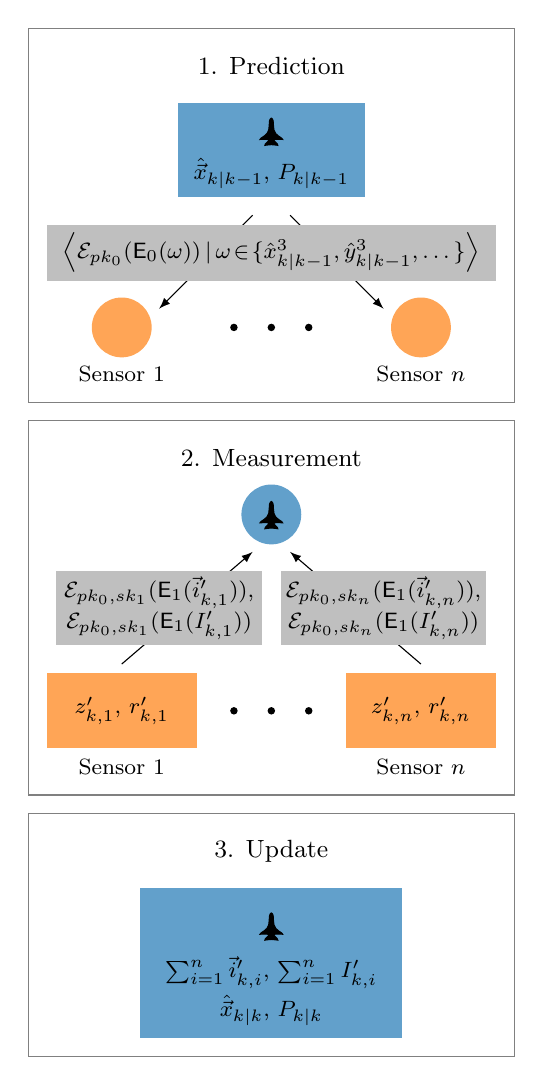
\begin{tikzpicture}[font=\footnotesize,scale=0.95]
    % Prediction
    \draw [gray] (0,3) rectangle (6.5,8);
    \node at (3.25,7.5) {\small 1. Prediction};

    % Navigator
    \fill  [pyplotblue!70] (2,7) rectangle (4.5,5.75);
    \pic[xscale=0.22,yscale=0.3] at (3.25,6.7975) {plane};
    \node at (3.25,6.0625) {$\hat{\vec{x}}_{k|k-1}$, $\mat{P}_{k|k-1}$};
    
    % Sensors
    \fill  (1.25,4) [pyplotorange!70] ellipse (0.4 and 0.4);
    \node at (1.25,3.375) {Sensor $1$};
    \fill  (5.25,4) [pyplotorange!70] ellipse (0.4 and 0.4);
    \node at (5.25,3.375) {Sensor $n$};
        
    \fill [black] (2.75,4) circle (0.05);
    \fill [black] (3.25,4) circle (0.05);
    \fill [black] (3.75,4) circle (0.05);
        
    % Arrows
    \draw [-latex] plot[smooth, tension=.7] coordinates {(3,5.5) (1.75,4.25)};
    \draw [-latex] plot[smooth, tension=.7] coordinates {(3.5,5.5) (4.75,4.25)};
    
    \fill [lightgray]  (0.25,5.375) rectangle (6.25,4.625);
    \node at (3.25,5) {$\left\langle\mathcal{E}_{pk_0}(\mathsf{E}_0(\omega)) \,|\, \omega \!\in\! \{\hat{x}^3_{k|k-1}, \hat{y}^3_{k|k-1}, \dots\}\right\rangle$};
    
    
    % Measurement
    \draw [gray] (0,-2.25) rectangle (6.5,2.75);
    \node at (3.25,2.25) {\small 2. Measurement};
    
    % Navigator
    \fill  (3.25,1.5) [pyplotblue!70] ellipse (0.4 and 0.4);
    \pic[xscale=0.22,yscale=0.3] at (3.25,1.6725) {plane};
        
    % Sensors
    \fill  [pyplotorange!70] (6.25,-1.625)  rectangle (4.25,-0.625);
    \node at (1.25,-1.875) {Sensor $1$};
    \fill  [pyplotorange!70] (2.25,-1.625)  rectangle (0.25,-0.625);
    \node at (5.25,-1.875) {Sensor $n$};
    
    \node at (1.25,-1.125) {$z'_{k,1}$, $r'_{k,1}$};
    \node at (5.25,-1.125) {$z'_{k,n}$, $r'_{k,n}$};
    
    \fill [black] (2.75,-1.125) circle (0.05);
    \fill [black] (3.25,-1.125) circle (0.05);
    \fill [black] (3.75,-1.125) circle (0.05);
    
    % Arrows
    \draw [-latex] plot[smooth, tension=.7] coordinates {(1.25,-0.5) (3,1)};
    \draw [-latex] plot[smooth, tension=.7] coordinates {(5.25,-0.5) (3.5,1)};
    
    \fill [lightgray]  (0.375,0.75) rectangle (3.125,-0.25);
    \node[align=center] at (1.75,0.25) {$\mathcal{E}_{pk_0,sk_1}(\mathsf{E}_1(\vec{i}'_{k,1}))$,\\$\mathcal{E}_{pk_0,sk_1}(\mathsf{E}_1(\mat{I}'_{k,1}))$};
    \fill [lightgray]  (3.375,0.75) rectangle (6.125,-0.25);
    \node[align=center] at (4.75,0.25) {$\mathcal{E}_{pk_0,sk_n}(\mathsf{E}_1(\vec{i}'_{k,n}))$,\\$\mathcal{E}_{pk_0,sk_n}(\mathsf{E}_1(\mat{I}'_{k,n}))$};
    
    
    % Update
    \draw [gray] (0,-5.75) rectangle (6.5,-2.5);
    \node at (3.25,-3) {\small 3. Update};
    
    % Navigator
    \fill  [pyplotblue!70] (1.5,-3.5) rectangle (5,-5.5);
    \pic[xscale=0.22,yscale=0.3] at (3.25,-3.8275) {plane};
    \node at (3.25,-4.625) {$\sum_{i=1}^n \vec{i}'_{k,i}$, $\sum_{i=1}^n\mat{I}'_{k,i}$};
    \node at (3.25,-5.125) {$\hat{\vec{x}}_{k|k}$, $\mat{P}_{k|k}$};
\end{tikzpicture}
\caption{Procedure at timestep $k$ for the proposed confidential range-only EIF.}
\label{fig:nonlin_fusion:alg_steps}
% TODO change the x and P to y and Y as per the EIF. Make parts subfigures as with the previous diagram.
\end{figure}

% 
%  ######      ######  ##          ###     ######   ######  
% ##    ##    ##    ## ##         ## ##   ##    ## ##    ## 
% ##          ##       ##        ##   ##  ##       ##       
%  ######     ##       ##       ##     ##  ######   ######  
%       ##    ##       ##       #########       ##       ## 
% ##    ##    ##    ## ##       ##     ## ##    ## ##    ## 
%  ######      ######  ######## ##     ##  ######   ######  
% 

\subsection{Solvable Sub-Class of Non-Linear Measurement Models}\label{subsec:nonlin_fusion:solvable_nonlin_class}
So far in this chapter, we have presented a method for measurement fusion in the context of range-only navigation that meets our desired security goals. As originally introduced, this solution aims to establish the foundations for a general fusion method for non-linear measurements that achieves the same data confidentiality guarantees and can itself be generalised to solving a sub-class of non-linear measurement problems not limited to range-only navigation. Recalling our aim of rewriting \eqref{eq:nonlin_fusion:measurement_vec} and \eqref{eq:nonlin_fusion:measurement_mat} as a linear combination of functions of $\hat{\vec{x}}_{k|k-1}$, and noting that this was possible when the measurement function $h_i$ could be rewritten in the same way, a more general solution can be seen. That is, \textit{any} non-linear measurement functions $\vec{h}_{k,i}$ that can be written in the form
\begin{equation}\label{eq:nonlin_fusion:measurement_func_of_solvable_class}
    \vec{h}_{k,i}(\vec{x}) = \sum_{j=1}^\nu a_j\vec{\mathcal{H}}_j(\vec{x})\,,
\end{equation}
where all functions $\vec{\mathcal{H}}_j$, $1\leq j\leq \nu$, do not depend on any sensitive sensor information, are sufficient for rearranging measurement vectors and matrices, $\vec{i}_{k, i}$ and $\mat{I}_{k, i}$, in a similar form and applying the scheme in section \ref{sec:nonlin_fusion:lcao_scheme} to the distributed fusion problem. 

To stress the applicability of the solution to this sub-class of non-linear problems, we note that the presented solution with range-only measurements does not directly fit into this category as shown in section \ref{subsec:nonlin_fusion:measurement_modification}, requiring a modification to measurements to achieve the desired form in \eqref{eq:nonlin_fusion:measurement_func_of_solvable_class}. Similarly, other non-linear measurements that do not directly suit the required form but can be modified accordingly are also solvable by the presented method.

% 
%  ######  ########  ######  
% ##    ## ##       ##    ## 
% ##       ##       ##       
%  ######  ######   ##       
%       ## ##       ##       
% ##    ## ##       ##    ## 
%  ######  ########  ######  
% 

\subsection{Security Analysis}\label{subsec:nonlin_fusion:security}
With the confidential EIF defined, we can interpret the aggregation leakage of an LCAO scheme in the context of range sensor localisation. The leakage function from the $\mathsf{AggDec}$ algorithm corresponds to the information vector and matrix sums, $\sum_{i=1}^n\vec{i}'_{k, i}$ and $\sum_{i=1}^n\mat{I}'_{k, i}$, respectively, but recalling that a compromised navigator can learn the individual sums weighted by the same weight, sums
\begin{equation*}
    \left\{\sum_{i=1}^n2r^{-1}_{k, i},\ \sum_{i=1}^n-r^{-1}_{k, i}s_{x, i},\ \sum_{i=1}^n-2r^{-1}_{k, i}s_{x, i},\ \dots\right\}
\end{equation*}
can be leaked as well. From this leakage, we can see that sensitive sensor information, $z'_{k, i}$, $r'_{k, i}$ and $\vec{s}_i$, is present only in their complete sums

\begin{equation}\label{eq:nonlin_fusion:localisation_leakage}
    \sum_{i=1}^nz'_{k,i}\,,\ \sum_{i=1}^nr'_{k,i}\,,\ \sum_{i=1}^ns_{x,i} \text{ and } \sum_{i=1}^ns_{y,i}\,,
\end{equation}
which in practice can be interpreted as their averages. Therefore, in the context of our proposed localisation method, LCAO leakage corresponds to the averages of sensors' sensitive information, while individual sensor information remains private.
% TODO extend to the general case from the previous subsection

% 
%  ######  #### ##     ## 
% ##    ##  ##  ###   ### 
% ##        ##  #### #### 
%  ######   ##  ## ### ## 
%       ##  ##  ##     ## 
% ##    ##  ##  ##     ## 
%  ######  #### ##     ## 
% 

\subsection{Simulation}\label{subsec:nonlin_fusion:simulation}
As well as having shown the theoretical backing for the security of our scheme, we have simulated the proposed localisation method to evaluate its performance. A two-dimensional, linear, constant-velocity system model,
\begin{equation*}
    \vec{x}_{k} = 
    \begin{bmatrix}
        1 & 0 & 0.5 & 0\\
        0 & 1 & 0 & 0.5\\
        0 & 0 & 1 & 0\\
        0 & 0 & 0 & 1
    \end{bmatrix} \cdot \vec{x}_{k-1} + \vec{w}_k\,,
\end{equation*}
where noise term $\vec{w}_k \sim \mathcal{N}(\vec{0}, \mat{Q})$ and
\begin{equation*}
    \mat{Q} = \frac{1}{10^3} \cdot
    \begin{bmatrix}
        0.4 & 0 & 1.3 & 0\\
        0 & 0.4 & 0 & 1.3\\
        1.3 & 0 & 5.0 & 0\\
        0 & 1.3 & 0 & 5.0
    \end{bmatrix}\,,
\end{equation*}
was simulated and tracked with the algorithms in section~\ref{subsec:nonlin_fusion:pseudocode}, using a linear Kalman filter for the navigator's local state prediction. Code was written in the C programming language using the MPI library [theopenmpiprojectOpenMPI2020] to support asynchronous computations by the sensors and the navigator. The MG1 mask generation function and the SHA256 hash function, from the OpenSSL library [theopensslprojectOpenSSL2020], were used to implement the required hash function $H$, and the Libpaillier library [bethencourtLibpaillier2010] was used for the Paillier encryption scheme. Additionally, GNU libraries, GSL [thegsldevelopmentteamGSLGNUScientific2019] and GMP [granlundGMPGNUMultiple2020], were used for algebraic operations and multiple-precision encoded integers, respectively. All execution was performed on a 3.33GHz Xeon W3680 CPU, running on the Windows Subsystem for Linux (WSL).

We have considered multiple sensor layouts, each with four sensors, to capture the dependence of estimated modified measurement variances $r'_{k,i}$ on the original measurements $z_{k,i}$. These layouts of varying sensor distances are shown next to the simulation initial state and a sample track in figure \ref{fig:sim_layouts}.
\begin{figure}[htbp]
    \centering
    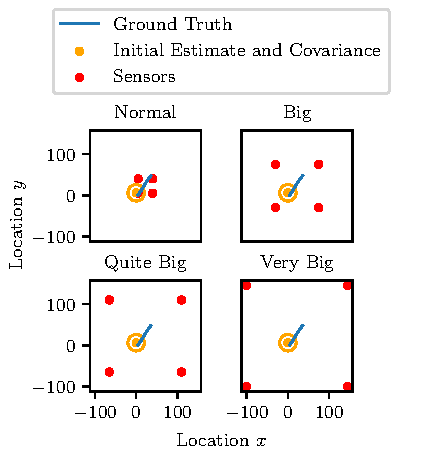
\includegraphics{figures/layouts.pdf}
    \caption{Different simulation layouts with varying distances between navigator and sensors.}
    \label{fig:sim_layouts}
\end{figure}
To demonstrate the accuracy of the method, we have compared the root mean square error (RMSE) of the privacy-preserving filter to the standard EIF using unmodified measurements, which is algebraically equivalent to the EKF typically used in industry for linearising non-linear state estimation. Estimation in each layout from figure \ref{fig:sim_layouts} consisted of $50$ filter iterations and was run $1000$ times. Unmodified measurement variances were taken as $r_{k,i}=5$ for all $k>0$ and a large fractional precision factor, $\phi=2^{32}$, was chosen. The results can be seen in figure \ref{fig:sim_layout_errors}.
\begin{figure}[htbp]
    \centering
    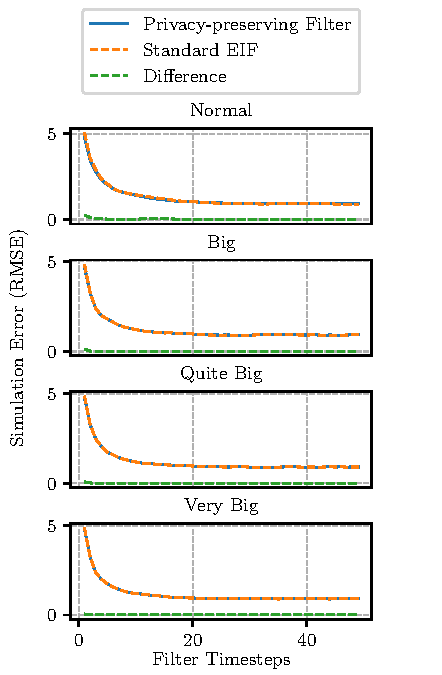
\includegraphics{figures/layout_errors.pdf}
    \caption{Average RMSE of our privacy-preserving filter and the standard EIF for different layouts.}
    \vspace{-\baselineskip}
    \label{fig:sim_layout_errors}
\end{figure}
From these results, we can see a strong similarity in filter performance between the privacy-preserving method and that of the traditional EIF. We can also see that the varying average distances between sensors and the navigator have little impact on the differences in performance. We attribute this similarity in RMSE to the conservativeness of estimated modified measurement variances $r'_{k,i}$, eliminating additional filter divergences, and to the high fractional precision factor, keeping computations consistent with the floating-point arithmetic of the EIF.

In addition to filter error, computational performance is important to consider when relying on cryptographic methods. Figure \ref{fig:sim_timing} shows the averages of $10$ execution times when varying the numbers of sensors and key sizes (bit lengths of $N$). Here, increasing the number of sensors primarily affects the number of inter-process communications and aggregation steps due to the asynchronous implementation.
\begin{figure}[htbp]
    \centering
    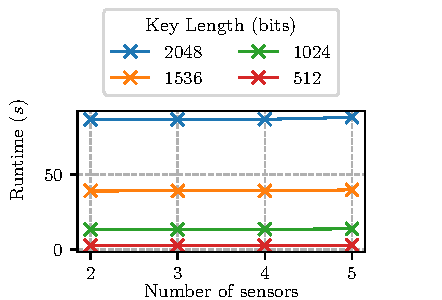
\includegraphics{figures/timing.pdf}
    \caption{Runtimes for varying key sizes and numbers of sensors.}
    \label{fig:sim_timing}
\end{figure}
We can see that the predominant computational costs stem from cryptographic computations and are directly dependent on the chosen key size. In practice, choosing a key size should take into account the duration of secrecy and the secret key lifetime. When relying on the DCRA for security, the current recommendation for encrypting government documents is the use of $2048$ bit length keys [barkerRecommendationPairwiseKey2019]. For our implementation and aforementioned hardware, this results in a filter update roughly every $1.7s$. In a scenario where sensors are mobile and past navigations can be made public, reduced key sizes can be considered, while a further decrease in computation time could be achieved with code optimisations and more powerful hardware.

% 
%  .d8888b.   .d88888b.  888b    888  .d8888b.  
% d88P  Y88b d88P" "Y88b 8888b   888 d88P  Y88b 
% 888    888 888     888 88888b  888 888    888 
% 888        888     888 888Y88b 888 888        
% 888        888     888 888 Y88b888 888        
% 888    888 888     888 888  Y88888 888    888 
% Y88b  d88P Y88b. .d88P 888   Y8888 Y88b  d88P 
%  "Y8888P"   "Y88888P"  888    Y888  "Y8888P"  
%                                               
%                                               
%                                               
% 

\section{Conclusions on Confidential Distributed Non-Linear Measurement Fusion}\label{sec:nonlin_fusion:conclusion}
We have presented a localisation filter in the presence of range-only sensors, which preserves both navigator and sensor privacies. A suitable cryptographic scheme has been introduced and a filter implementation compared and evaluated. Privacy-preserving range-only localisation is suitable for use in environments where sensor networks are untrusted or location is considered private and we hope to extend the method to broader measurement models in the future. Additional future work includes exploring more computationally efficient encryption schemes, the security implications of sensors that are not only honest-but-curious and expanding the LCAO notion to enforce the consistent broadcast assumption.

\chapter{Provable Estimation Performances}\label{ch:priv_estimation}

% 
% 8888888b.  8888888b.   .d88888b.  888888b.   
% 888   Y88b 888   Y88b d88P" "Y88b 888  "88b  
% 888    888 888    888 888     888 888  .88P  
% 888   d88P 888   d88P 888     888 8888888K.  
% 8888888P"  8888888P"  888     888 888  "Y88b 
% 888        888 T88b   888     888 888    888 
% 888        888  T88b  Y88b. .d88P 888   d88P 
% 888        888   T88b  "Y88888P"  8888888P"  
%                                              
%                                              
%                                              
% 

\section{Problem Formulation}\label{sec:priv_estimation:problem}
In this chapter, we look at the problem of formalising estimation performances from a cryptographic perspective and allowing meaningful cryptographic guarantees when comparing estimators. The scenario that we will use to build this formalisation is one where system and measurement models are known and stochastic, and state estimators can have access to secret keys, providing them with a certain privilege. Estimators holding no keys are termed unprivileged. Our goal is to develop a single-sensor scheme that quantifies and cryptographically guarantees a difference between privileged and unprivileged estimator performances when both estimators have access to the same measurements and when models are Gaussian and linear. Further, we look at the extension to multiple sensors and the effect of fusion on cryptographic estimation performance guarantees as well as the applicability of the method to non-linear models.

To capture the aim of comparing a privileged and unprivileged estimator, we first define how to assess the estimation difference between them, and which algorithms are required to characterise a privileged estimation scheme. After giving relevant formal cryptographic definitions, the considered single-sensor privileged estimation problem and its extension to multiple sensors are presented.

% 
%  ######  ########  ##    ## ########  ########  #######     ########  ########   #######  ########  
% ##    ## ##     ##  ##  ##  ##     ##    ##    ##     ##    ##     ## ##     ## ##     ## ##     ## 
% ##       ##     ##   ####   ##     ##    ##    ##     ##    ##     ## ##     ## ##     ## ##     ## 
% ##       ########     ##    ########     ##    ##     ##    ########  ########  ##     ## ########  
% ##       ##   ##      ##    ##           ##    ##     ##    ##        ##   ##   ##     ## ##     ## 
% ##    ## ##    ##     ##    ##           ##    ##     ##    ##        ##    ##  ##     ## ##     ## 
%  ######  ##     ##    ##    ##           ##     #######     ##        ##     ##  #######  ########  
% 

\subsection{Formal Cryptographic Problem}\label{subsec:priv_estimation:crypto_problem}
While we later introduce assumptions on the system and measurement models, it is more practical to define a broader security notion that can be satisfied under arbitrary specified conditions on the models. This lends the use of the notion to future literature and is more in line with typical cryptographic practice.

We aim to give the security notion in terms of probabilistic polynomial-time (PPT) attackers and capture the desired leakage as well as attacker capabilities. The most commonly desired leakage, cryptographic indistinguishability, is not suitable for our scenario due to our desire for both estimators to gain \textit{some} information from measurements. Instead, we define security in terms of a time series of semi-definite matrices, given arbitrary known models, such that the difference in estimation error covariances between the estimators with and without access to a privilege, respectively, is bounded by the series at all times.

To formalize this, we introduce the following notations and definitions. We assume the existence of an arbitrary process (not necessarily Gaussian or linear) following a known system model exactly, with the state at timestep $k$ denoted by $\vec{x}_k\in\mathbb{R}^d$ and model parameters $\mathcal{M}_{\mathsf{S}}$. Similarly, we assume the existence of a means of process measurement following a known measurement model exactly, with the measurement at timestep $k$ denoted by $\vec{z}_k\in\mathbb{R}^m$ and model parameters $\mathcal{M}_{\mathsf{M}}$. We can now define a relevant scheme.
\begin{definition}
    A \textit{privileged estimation scheme} is a pair of probabilistic algorithms $(\mathsf{Setup},\mathsf{Noise})$, given by
    \begin{description}
        \item[$\mathsf{Setup}(\mathcal{M}_{\mathsf{S}}, \mathcal{M}_{\mathsf{M}}, \kappa)$] On the input of models $\mathcal{M}_{\mathsf{S}}$ and $\mathcal{M}_{\mathsf{M}}$, and the security parameter $\kappa$, public parameters $\mathsf{pub}$ and a secret key $\mathsf{sk}_{\mathsf{g}}$ are created.
        \item[$\mathsf{Noise}(\mathsf{pub}, \mathsf{sk}_{\mathsf{g}}, k, \mathcal{M}_{\mathsf{S}}, \mathcal{M}_{\mathsf{M}}, \vec{z}_1, \dots, \vec{z}_k)$] On input of public parameters $\mathsf{pub}$, secret key $\mathsf{sk}_{\mathsf{g}}$, timestep $k$, models $\mathcal{M}_{\mathsf{S}}$ and $\mathcal{M}_{\mathsf{M}}$, and measurements $\vec{z}_1,\dots,\vec{z}_k$, a privileged and unprivileged modified measurement (with no required model constraints) are returned, $\vec{z}_k^{\{\mathsf{p}\}}$ and $\vec{z}_k^{\{\mathsf{up}\}}$, respectively.
    \end{description}
\end{definition}
In addition to the scheme above, we also give the following definitions to help formalize our desired security notion.
\begin{definition}\label{def:priv_estimation:crypto_estimator}
    An \textit{estimator} is any probabilistic algorithm that produces a guess of the state $\vec{x}_k$ for a given timestep $k$.
\end{definition}
\begin{definition}\label{def:priv_estimation:negligible_covariance}
    A \textit{negligible covariance function},
    \begin{equation}
        \mathsf{neglCov}_m(\kappa):\mathbb{N}\rightarrow \mathbb{R}^{m\times m}\,,
    \end{equation}
    is a function that returns a matrix $\mat{A}$ such that $\mat{A}$ is a valid covariance ($\mat{A}\succ 0$ and $\mat{A}=\mat{A}^\top$) and for each of its eigenvalues $a\in\mathsf{eig}(\mat{A})$, there exists a negligible function [Def. 3.4][katzIntroductionModernCryptography2008] $\eta$ such that $a\leq\eta(\kappa)$.
\end{definition}

Now we can give the security notion that captures the formal requirements of the estimation difference we want to capture.
\begin{definition}\label{def:priv_estimation:covariance_privilege_notion}
    A privileged estimation scheme meets the notion \textit{$\{\mat{D}_1,\mat{D}_2,\dots\}$-Covariance Privilege for Models $\mathcal{M}_{\mathsf{S}}$ and $\mathcal{M}_{\mathsf{M}}$} if for any PPT estimator $\mathcal{A}$, there exists a PPT estimator $\mathcal{A}^\prime$, such that
    \begin{equation}\label{eq:priv_estimation:covariance_privilege}
        \begin{split}
            &\mathsf{Cov}\left[\mathcal{A}\left(k, \kappa, \mathsf{pub}, \mathcal{M}_S, \mathcal{M}_M, \vec{z}_1^{\{\mathsf{up}\}},\dots,\vec{z}_k^{\{\mathsf{up}\}}\right) - \vec{x}_k \right]\\
            &-\mathsf{Cov}\left[\mathcal{A}^\prime\left(k, \kappa, \mathsf{pub}, \mathcal{M}_S, \mathcal{M}_M, \vec{z}_1^{\{\mathsf{p}\}},\dots,\vec{z}_k^{\{\mathsf{p}\}}\right) - \vec{x}_k \right]\\
            &\quad\succeq \mat{D}_k - \mathsf{neglCov}_m(\kappa)
        \end{split}
    \end{equation}
   for all $k>0$, some negligible covariance function and where matrices $\mat{D}_k$ are semi-definite, \textit{i.e.} $\mat{D}_k\preceq 0$ or $\mat{D}_k\succeq 0$. Here, estimators $\mathcal{A}$ and $\mathcal{A}^\prime$ are running in polynomial-time with respect to the security parameter $\kappa$, and all probabilities are taken over randomness introduced in models $\mathcal{M}_{\mathsf{S}}$ and $\mathcal{M}_{\mathsf{M}}$, estimators $\mathcal{A}$ and $\mathcal{A}^\prime$, and algorithms $\mathsf{Setup}$ and $\mathsf{Noise}$.
\end{definition}

Informally, the above definition states that no estimator that can only access unprivileged measurements $\vec{z}_1^{\{\mathsf{up}\}},\dots,\vec{z}_k^{\{\mathsf{up}\}}$ can estimate a state $\vec{x}_k$ for a timestep $k$ with a mean square error (MSE) covariance less than an equivalent estimator with access to privileged measurements $\vec{z}_1^{\{\mathsf{p}\}},\dots,\vec{z}_k^{\{\mathsf{p}\}}$, by a margin of at least $\mat{D}_k$. We also note that by taking probabilities over randomness introduced in the system model, and therefore the possible true states $\vec{x}_k$, the definition fits a Bayesian interpretation of probability for any stochastic system model.

% 
% ########  ######  ########    ########  ########   #######  ########  
% ##       ##    ##    ##       ##     ## ##     ## ##     ## ##     ## 
% ##       ##          ##       ##     ## ##     ## ##     ## ##     ## 
% ######    ######     ##       ########  ########  ##     ## ########  
% ##             ##    ##       ##        ##   ##   ##     ## ##     ## 
% ##       ##    ##    ##       ##        ##    ##  ##     ## ##     ## 
% ########  ######     ##       ##        ##     ##  #######  ########  
% 

\subsection{Estimation Problem}\label{subsec:priv_estimation:estimation_problem}
To make use of the introduced cryptographic notion, we consider specific estimation models to use in the single-sensor case when developing a privileged estimation scheme with a provable estimation performance difference between privileged and unprivileged estimators. A system model gives the state $\vec{x}_k\in\mathbb{R}^d$ at an integer timestep $k$ and is given by
\begin{equation}\label{eq:priv_estimation:system_model}
    \vec{x}_k = \mat{F}_k\vec{x}_{k-1} + \vec{w}_k\,,
\end{equation}
with noise term $\vec{w}_k\sim \mathcal{N}(\vec{0}, \mat{Q}_k)$ and a known non-zero covariance $\mat{Q}_k\in \mathbb{R}^{d\times d}$. Similarly, the measurement model gives a measurement $\vec{z}_k$ at a timestep $k$ and is given by
\begin{equation}\label{eq:priv_estimation:single_sensor_measurement_model}
    \vec{z}_k = \mat{H}_k\vec{x}_k + \vec{v}_k\,,
\end{equation}
with noise term $\vec{v}_k\sim \mathcal{N}(\vec{0}, \mat{R}_k)$ and a known non-zero covariance $\mat{R}_k\in \mathbb{R}^{m\times m}$.

In this scenario, the sensor holds a secret key $\mathsf{sk}_{\mathsf{g}}$ that it uses to modify its measurements, and privileged estimators hold this shared key while unprivileged estimators do not. We also assume that sensors and estimators are synchronised in timestep $k$ to simplify later cryptographic evaluation.% Lastly, an extension to a single-sensor multiple-privilege scheme is also considered and discussed further in section \ref{sec:priv_estimation:privileged_estimation}.

% 
% ######## ##     ##  ######     ########  ########   #######  ########  
% ##       ##     ## ##    ##    ##     ## ##     ## ##     ## ##     ## 
% ##       ##     ## ##          ##     ## ##     ## ##     ## ##     ## 
% ######   ##     ##  ######     ########  ########  ##     ## ########  
% ##       ##     ##       ##    ##        ##   ##   ##     ## ##     ## 
% ##       ##     ## ##    ##    ##        ##    ##  ##     ## ##     ## 
% ##        #######   ######     ##        ##     ##  #######  ########  
% 

\subsection{Multi-Sensor Problem}\label{subsec:priv_estimation:fusion_problem}
As well as the single-sensor problem, we are also interested in the extension to environments with multiple sensors, where the fusion of measurements can also lead to better estimation performance irrespective of privilege. Here, we only consider multiple privileges, such that estimators with a higher privilege should perform better than those with a lower one while taking into consideration the estimation benefits from fusing additional measurements. We again consider linear and Gaussian models, where the state $\vec{x}_k \in \mathbb{R}^d$ follows the system model \eqref{eq:priv_estimation:system_model}. Measurements $\vec{z}_{k,i} \in \mathbb{R}^m$ are now indexed by sensor $i$, $1\leq i\leq n$, and follow the measurement models
\begin{equation}\label{eq:priv_estimation:multi_sensor_measurement_models}
    \vec{y}_{k,i} = \mat{H}_{k,i} \vec{x}_k + \vec{v}_{k,i}\,,
\end{equation}
with noise terms $\vec{v}_{k,i} \sim \mathcal{N}(\vec{0},\mat{R}_{k,i})$ and known non-zero covariances $\mat{R}_{k,i} \in \mathbb{R}^{m \times m}$. In addition to these models, we again assume synchronisation, between all estimators and sensors $i$, in timesteps $k$, simplifying later cryptographic evaluation.

Now, each sensor holds its own secret key $\mathsf{sk}_{\mathsf{g}, i}$, $1\leq i\leq n$, which is shared with estimators of appropriate privileges. The privileges that we consider, in terms of access to keys and measurements, will be defined by sequential sensor access. That is, in the presence of $n$ sensors, we will consider exactly $n$ possible privilege levels, where each privilege $\pi>0$ corresponds to holding the sequential secret keys $\mathsf{sk}_{\mathsf{g},j}$, $1\leq j\leq \pi$, while being unprivileged, $\pi=0$, corresponds to holding none. Additionally, we assume that estimators have access to all privileged measurements, those from sensors whose keys they hold, but can fuse additional unprivileged measurements, from those whose keys they do not hold. To simplify notation, we consider access to unprivileged measurements to be sequential as well, and can therefore capture estimator capabilities by letting $\mathsf{e}^{[\pi,\tau]}$ denote an estimator with privilege $\pi$ and access to measurements from $\tau\geq\pi$ sensors $i$, $1\leq i\leq \tau$.

Multiple measurements and the effects of privilege and fusion on estimation performance complicate the cryptographic analysis in the case of multiple sensors. To demonstrate that a presented scheme guarantees better performance for higher privilege estimators while limiting the benefit from fusing unprivileged measurements, the covariance privilege notion in section \ref{subsec:priv_estimation:crypto_problem} will be used to guarantee two estimation performance differences for each privilege $\pi$.
\begin{description}
    \item[Performance Loss Lower Bound] Here, we aim to guarantee a lower bound on the estimation performance loss of any unprivileged estimator $\mathsf{e}^{[0, n]}$ on a privilege-$\pi$ estimator $\mathsf{e}^{[\pi,\pi]}$. Naturally, this will remain a lower bound when unprivileged estimators have access to fewer unprivileged measurements or privileged estimators have access to more.
    \item[Performance Gain Upper Bound] This bound aims to guarantee an upper bound on the estimation performance gain of any estimator $\mathsf{e}^{[\pi, n]}$ on a privilege-$\pi$ estimator $\mathsf{e}^{[\pi,\pi]}$. The bound similarly remains an upper bound when fewer unprivileged measurements are fused.
\end{description}
Lastly, a suitable scheme should be one with at least two free parameters responsible for controlling the values of these two bounds.
\begin{remark}
  We stress that the two bounds that will be guaranteed only bound the performances of estimators of the specified forms. That is, nothing is said about estimators which may corrupt sensors to obtain keys beyond their privilege or additional unprivileged measurements. Bounds on leakage caused by corrupting sensors can in some cases be captured by estimators of a new form $\mathsf{e}^{[\pi^\prime,\tau^\prime]}$, but are in general beyond the scope of this thesis.
\end{remark}


% 
% 8888888b.  8888888b.  8888888 888     888      8888888888 .d8888b. 88888888888 
% 888   Y88b 888   Y88b   888   888     888      888       d88P  Y88b    888     
% 888    888 888    888   888   888     888      888       Y88b.         888     
% 888   d88P 888   d88P   888   Y88b   d88P      8888888    "Y888b.      888     
% 8888888P"  8888888P"    888    Y88b d88P       888           "Y88b.    888     
% 888        888 T88b     888     Y88o88P        888             "888    888     
% 888        888  T88b    888      Y888P         888       Y88b  d88P    888     
% 888        888   T88b 8888888     Y8P          8888888888 "Y8888P"     888     
%                                                                                
%                                                                                
%                                                                                
% 

\section{Privileged Estimation for Linear Systems}\label{sec:priv_estimation:privileged_estimation}
In this section, we propose a privileged estimation scheme meeting the security notion in section \ref{subsec:priv_estimation:crypto_problem} for a derivable series of semi-definite matrices when models $\mathcal{M}_{\mathsf{S}}$ and $\mathcal{M}_{\mathsf{M}}$ are given by \eqref{eq:priv_estimation:system_model} and \eqref{eq:priv_estimation:single_sensor_measurement_model}, respectively. The key idea behind the method is to add pseudorandom Gaussian noise to existing measurement noise at the sensor, degrading estimation at estimators that cannot remove it. This added noise is a keystream generated by the sensor's secret key and can only be removed from measurements by an estimator holding the same key.

% 
% ##    ## ######## ##    ##  ######  ######## ########  ########    ###    ##     ## 
% ##   ##  ##        ##  ##  ##    ##    ##    ##     ## ##         ## ##   ###   ### 
% ##  ##   ##         ####   ##          ##    ##     ## ##        ##   ##  #### #### 
% #####    ######      ##     ######     ##    ########  ######   ##     ## ## ### ## 
% ##  ##   ##          ##          ##    ##    ##   ##   ##       ######### ##     ## 
% ##   ##  ##          ##    ##    ##    ##    ##    ##  ##       ##     ## ##     ## 
% ##    ## ########    ##     ######     ##    ##     ## ######## ##     ## ##     ## 
% 

\subsection{Gaussian Keystream}\label{subsec:priv_estimation:est_gaussian_keystream}
To generate the desired pseudorandom Gaussian noise that can be added to existing measurements, the sensor first generates a typical cryptographic pseudorandom bitstream with its secret key $\mathsf{sk}_{\mathsf{g}}$. This can be done with any cryptographic stream cipher and reduces the security of the method to a single, well-studied and replaceable component. This bitstream can be interpreted as sequential pseudorandom integers of a suitable size and used to generate a sequence of pseudorandom uniform real numbers $\upsilon_t\ \dot{\sim}\ \mathcal{U}(0,1)$ for sequence indices $t>0$.

Here, we note that the conversion to real numbers $\upsilon_t$ is cryptographically non-trivial due to floating-point representation affecting the pseudorandomness of the samples, and complicating the meeting of a desired cryptographic notion. Instead, we assume that floating-point numbers are sufficiently close to real numbers and rely on any common method for choosing the bit size of pseudorandom integers and the generation of uniform numbers $\upsilon_t$ [goualardGeneratingRandomFloatingPoint2020]. This assumption will be further discussed with the security of the presented scheme in section \ref{subsec:priv_estimation:est_security}.

With this assumption, we are left with generating a series of pseudorandom standard normal Gaussian samples, which can be readily computed using the Box-Muller transform [paleyFourierTransformsComplex1934]. This is given by
\begin{equation}
    \psi_t = \sqrt{-2\ln (\upsilon_t)}\cos(2\pi \upsilon_{t+1})
\end{equation}
and
\begin{equation}
    \psi_{t+1} = \sqrt{-2\ln (\upsilon_t)}\sin(2\pi \upsilon_{t+1})\,,
\end{equation}
obtaining two, independent, standard normal Gaussian samples from two uniform ones. To generate noise that can be added by the sensor and removed by a privileged estimator using this series, a conversion to a $d$-dimension zero-mean multivariate Gaussian sample is required at every timestep $k$. As control over the difference in estimation error between privileged and unprivileged estimators is desired, a symmetric matrix parameter $\mat{S}\succ 0$ is introduced, such that added pseudorandom noise $\vec{g}_k$ follows distribution $\vec{g}_k\ \dot{\sim}\ \mathcal{N}(\vec{0},\mat{S})$. Given $\mat{S}$, $\vec{g}_k$ can be computed using the next $d$ Gaussian keystream samples,
\begin{equation}\label{eq:priv_estimation:est_gaussian_standard_noise_stream}
    \vec{\psi}_k =
    \begin{bmatrix}
        \psi_{(k-1)d+1} & \dots & \psi_{kd}
    \end{bmatrix}^\top\,,
\end{equation}
as
\begin{equation}\label{eq:priv_estimation:est_gaussian_noise_stream}
    \vec{g}_k = \mat{S}^{\frac{1}{2}}\vec{\psi}_k
\end{equation}
for any matrix $\mat{S}^{\frac{1}{2}}$ such that $\mat{S}^{\frac{1}{2}}\mat{S}^{\frac{1}{2}\top}=\mat{S}$. We also note that for the correct removal of noise terms $\vec{g}_k$ by the privileged estimator, index information $k$ is required but available when sensors and estimators are synchronised, as per the problem definition.

% 
% ##     ##  #######  ########  
% ###   ### ##     ## ##     ## 
% #### #### ##     ## ##     ## 
% ## ### ## ##     ## ##     ## 
% ##     ## ##     ## ##     ## 
% ##     ## ##     ## ##     ## 
% ##     ##  #######  ########  
% 

\subsection{Measurement Modification}\label{subsec:priv_estimation:est_measurement_mod}
Using the noise in \eqref{eq:priv_estimation:est_gaussian_noise_stream}, the sensor can now modify measurements $\vec{z}_k$ by
\begin{equation}\label{eq:priv_estimation:est_modified_measurement}
    \vec{z}^\prime_k = \vec{z}_k + \vec{g}_k\,,
\end{equation}
resulting in a new measurement model
\begin{equation}
    \vec{z}^\prime_k = \mat{H}_k\vec{x}_k + \vec{v}_k + \vec{g}_k\,,
\end{equation}
with noise terms $\vec{v}_k\sim \mathcal{N}(\vec{0},\mat{R}_k)$ and $\vec{g}_k\ \dot{\sim}\ \mathcal{N}(\vec{0},\mat{S})$. This leads to two estimation problems for the privileged and unprivileged estimators, respectively.
\begin{description}
    \item[Privileged estimation] An estimator that holds the secret key $\mathsf{sk}_{\mathsf{g}}$ can compute the Gaussian key stream $\psi_t$, $t>0$, and therefore the added noise vectors $\vec{g}_k$ at every timestep $k$. Given the modified measurements \eqref{eq:priv_estimation:est_modified_measurement}, computing $\vec{z}_k = \vec{z}^\prime_k - \vec{g}_k$  obtains measurements following the measurement model \eqref{eq:priv_estimation:single_sensor_measurement_model} exactly.
    \item[Unprivileged estimation] In the case where pseudorandomness is indistinguishable from randomness, as is the case for an unprivileged estimator when a cryptographically secure keystream is used and the secret key $\mathsf{sk}_{\mathsf{g}}$ is not known, modified measurements are indistinguishable from those following the unprivileged measurement model 
    \begin{equation}\label{eq:priv_estimation:est_unpriv_measurement_model}
        \vec{z}^\prime_k = \mat{H}_k\vec{x}_k + \vec{v}^\prime_k\,,
    \end{equation}
   with $\vec{v}^\prime_k\sim \mathcal{N}(\vec{0},\mat{R}_k+\mat{S})$, exactly.
\end{description}

Intuitively, we can see that the two types of estimators have the difference between their estimation errors dependent on matrix $\mat{S}$.

% 
%  ######  ########  ######  
% ##    ## ##       ##    ## 
% ##       ##       ##       
%  ######  ######   ##       
%       ## ##       ##       
% ##    ## ##       ##    ## 
%  ######  ########  ######  
% 

\subsection{Security Analysis}\label{subsec:priv_estimation:est_security}
Recalling definition \ref{def:priv_estimation:covariance_privilege_notion}, we aim to show how the notion is met by the proposed estimation scheme. Before the proof sketch, we look at our scheme in the context of a formal privileged estimation scheme with model constraints and give some relevant optimality properties.

We consider the stochastic system model \eqref{eq:priv_estimation:system_model} and measurement model \eqref{eq:priv_estimation:single_sensor_measurement_model} exactly, that is, any linear models with known covariance, zero-mean, Gaussian additive noises. We define these as our model conditions and capture all relevant parameters in the respective equations in $\mathcal{M}_{\mathsf{S}}$ and $\mathcal{M}_{\mathsf{M}}$. Our scheme meets the definition of a formal privileged estimation scheme by defining the required algorithms $\mathsf{Setup}$ and $\mathsf{Noise}$ as
\begin{description}
    \item[$\mathsf{Setup}(\mathcal{M}_{\mathsf{S}}, \mathcal{M}_{\mathsf{M}}, \kappa)$] Initialize a cryptographically indistinguishable stream cipher with the parameter $\kappa$, set the secret key $\mathsf{sk}_{\mathsf{g}}$ to the stream cipher key and include an initial filter estimate $\hat{\vec{x}}_0$, error covariance $\mat{P}_0$ and added noise covariance $\mat{S}$ in the public parameters $\mathsf{pub}$.
    \item[$\mathsf{Noise}(\mathsf{pub}, \mathsf{sk}_{\mathsf{g}}, k, \mathcal{M}_{\mathsf{S}}, \mathcal{M}_{\mathsf{M}}, \vec{z}_1, \dots, \vec{z}_k)$] Using the stream cipher key $\mathsf{sk}_{\mathsf{g}}$ and public parameters $\mathsf{pub}$, create an unprivileged measurement by \eqref{eq:priv_estimation:est_modified_measurement}. Set and return the privileged measurement $\vec{z}^{\{\mathsf{p}\}}_k=\vec{z}_k$ and unprivileged measurement $\vec{z}^{\{\mathsf{up}\}}_k=\vec{z}^\prime_k$.
\end{description}
Here, we note that in the $\mathsf{Setup}$ algorithm above, the inclusion of an initial state estimate, its error covariance and the generated noise covariance in the public parameters $\mathsf{pub}$ are present only for the completeness of the cryptographic definition and not a requirement for the security of the scheme.

The idea behind our proof sketch relies on the optimality of the linear Kalman Filter (KF) introduced in section \ref{subsec:prelims:kf_opt}. Given an initial estimate and its error covariance, the KF produces updated estimates with the minimum mean square error (MSE) achievable for \textit{any} estimator when all measurements $\vec{z}_1,\dots,\vec{z}_k$ are observed, models are Gaussian and linear, and the same initialization is used. Since the KF also preserves the initial error covariance order,
\begin{equation}
   \mat{P}_k \preceq \mat{P}_k^\prime \implies \mat{P}_{k+1} \preceq \mat{P}_{k+1}^\prime\,,
\end{equation}
for two different filter estimate error covariances $\mat{P}_k$ and $\mat{P}_k^\prime$, we can define an error covariance lower-bound $\mat{P}_k^{(l)}$ for all possible initialisations by setting $\mat{P}_0^{(l)} = \mat{0}$ and computing the KF error covariance using the combined predict and update equations
\begin{equation}\label{eq:priv_estimation:est_lower_bound_error_cov}
    \begin{split}
        \mat{P}_k^{(l)} =& \Bigl( \mat{I} - (\mat{F}_k\mat{P}_{k-1}^{(l)}\mat{F}_k^\top + \mat{Q}_k)\mat{H}_k^\top \bigl(\mat{H}_k(\mat{F}_k\mat{P}_{k-1}^{(l)}\mat{F}_k^\top + \mat{Q}_k)\mat{H}_k^\top + \mat{R}_k\bigr)^{-1}\mat{H}_k\Bigr)\cdot\\
        &\quad\Bigl(\mat{F}_k\mat{P}_{k-1}^{(l)}\mat{F}_k^\top + \mat{Q}_k\Bigr)\,.
    \end{split}
\end{equation}
This gives us a lower bound at every timestep $k$, such that
\begin{equation}
    \mat{P}_k^{(l)} \preceq \mathsf{Cov}\left[\mathcal{A}\left(k, \mathcal{M}_{\mathsf{S}}, \mathcal{M}_{\mathsf{M}}, \vec{z}_1,\dots,\vec{z}_k\right) - \vec{x}_k \right]
\end{equation}
for \textit{any} estimator $\mathcal{A}$ following definition \ref{def:priv_estimation:crypto_estimator} and any Gaussian and linear models $\mathcal{M}_{\mathsf{S}}$ and $\mathcal{M}_{\mathsf{M}}$. This leads us to the proof sketch.

% 
% .########..########...#######...#######..########
% .##.....##.##.....##.##.....##.##.....##.##......
% .##.....##.##.....##.##.....##.##.....##.##......
% .########..########..##.....##.##.....##.######..
% .##........##...##...##.....##.##.....##.##......
% .##........##....##..##.....##.##.....##.##......
% .##........##.....##..#######...#######..##......
% 

\subsubsection{Proof Sketch}
We wish to show that the scheme in section \ref{subsec:priv_estimation:est_measurement_mod} meets $\{\mat{D}_1,\mat{D}_2,\dots\}$-Covariance Privilege for Models $\mathcal{M}_{\mathsf{S}}$ and $\mathcal{M}_{\mathsf{M}}$, for a computable series $\mat{D}_k$, $k>0$ dependent on a noise parameter $\mat{S}$, when $\mathcal{M}_{\mathsf{S}}$ and $\mathcal{M}_{\mathsf{M}}$ are Gaussian and linear. 

Since a cryptographically pseudorandom stream cipher is used, the stream integers, and therefore the uniform samples $\upsilon_t$ and normal Gaussian samples $\psi_t$, are indistinguishable from those generated from a truly random stream for any PPT estimator without the secret key. We persist with the previous assumption that floating-point representations of $\psi_t$ are sufficiently close to Gaussian and assume the KF to provide optimal estimation when using floating-point arithmetic. Using the $\mathsf{Setup}$ and $\mathsf{Noise}$ algorithms given in section \ref{subsec:priv_estimation:est_security} leads to pseudorandom measurements $\vec{z}^\prime_k$ that are indistinguishable from measurements following the unprivileged measurement model \eqref{eq:priv_estimation:est_unpriv_measurement_model}. We can then compute a lower-bound $\mat{P}_k^{\prime(l)}$ for any unprivileged estimator as $\mat{P}_0^{\prime(l)}=\mat{0}$ and
\begin{equation}\label{eq:priv_estimation:est_unprivileged_lower_bound_error_cov}
   \begin{split}
      \mat{P}_k^{\prime(l)} =& \Bigl( \mat{I} - (\mat{F}_k\mat{P}_{k-1}^{\prime(l)}\mat{F}_k^\top + \mat{Q}_k)\mat{H}_k^\top\bigl(\mat{H}_k(\mat{F}_k\mat{P}_{k-1}^{\prime(l)}\mat{F}_k^\top + \mat{Q}_k)\mat{H}_k^\top + \mat{R}_k+\mat{S}\bigr)^{-1}\mat{H}_k\Bigr)\cdot\\
      &\quad\Bigl(\mat{F}_k\mat{P}_{k-1}^{\prime(l)}\mat{F}_k^\top + \mat{Q}_k\Bigr)\,.
   \end{split}
\end{equation}
Taking the difference of \eqref{eq:priv_estimation:est_unprivileged_lower_bound_error_cov} and the lower bound error covariances for privileged estimators \eqref{eq:priv_estimation:est_lower_bound_error_cov} produces the series
\begin{equation}\label{eq:priv_estimation:est_covariance_difference_series}
   \mat{D}_k = \mat{P}_k^{\prime(l)} - \mat{P}_k^{(l)}\,,
\end{equation}
for $k>0$, which can be tuned by the parameter $\mat{S}$. Since both series $\mat{P}_k^{(l)}$ and $\mat{P}_k^{\prime(l)}$ give the lowest possible error covariance of the respective estimators, an estimator following the true model \eqref{eq:priv_estimation:single_sensor_measurement_model} can always be created for one following the unprivileged model \eqref{eq:priv_estimation:est_unpriv_measurement_model} such that their error covariances differ by at least $\mat{D}_k$ for each timestep $k$. A reduction proof can therefore be constructed, in which the existence of an unprivileged estimator that produces estimates such that \eqref{eq:priv_estimation:covariance_privilege} does not hold, implies the existence of an estimator with an error covariance lower than $\mat{P}_k^{\prime(l)}$ following model \eqref{eq:priv_estimation:est_unpriv_measurement_model}. As no such estimator exists, we conclude that our scheme meets $\{\mat{D}_1,\mat{D}_2,\dots\}$-Covariance Privilege for Models $\mathcal{M}_S$ and $\mathcal{M}_M$, when models are Gaussian and linear, concluding our proof sketch.

% 
% ....###.....######...######..##.....##.##.....##.########.
% ...##.##...##....##.##....##.##.....##.###...###.##.....##
% ..##...##..##.......##.......##.....##.####.####.##.....##
% .##.....##..######...######..##.....##.##.###.##.########.
% .#########.......##.......##.##.....##.##.....##.##.......
% .##.....##.##....##.##....##.##.....##.##.....##.##.......
% .##.....##..######...######...#######..##.....##.##.......
% 

\subsubsection{Implicit Assumptions}
In addition to the proof sketch, we stress some comments on accepting cryptographic guarantees in terms of estimation models $\mathcal{M}_{\mathsf{S}}$ and $\mathcal{M}_{\mathsf{M}}$ when used to estimate a physical process or approximate continuous models. The following assumptions are made in this scenario.
\begin{description}
    \item[Exact models] When assigning a model to a physical process, any cryptographic guarantees about the model assumes it describes the process \textit{exactly}. Often, models assume a Bayesian interpretation of probability (a stochastic state) or are chosen to simplify estimation, resulting in the possibility of better estimation given alternative or more complicated models. Although the standard for state estimation, we state the assumption to highlight the distinction between models and a physical process.
    \item[Floating-point approximation] As stated in section \ref{subsec:priv_estimation:est_gaussian_keystream} and the proof sketch above, floating-point approximations to real numbers complicate cryptographic guarantees when relying on proofs using real numbers such as KF optimality. While optimal estimation with floating-point numbers is beyond the scope of this thesis, their prevalence in the field of state estimation justifies the assumption of sufficient similarity and the insignificance of associated error introduced to the security notion.
\end{description}

% 
% .##....##..#######..##....##.........##.......####.##....##
% .###...##.##.....##.###...##.........##........##..###...##
% .####..##.##.....##.####..##.........##........##..####..##
% .##.##.##.##.....##.##.##.##.#######.##........##..##.##.##
% .##..####.##.....##.##..####.........##........##..##..####
% .##...###.##.....##.##...###.........##........##..##...###
% .##....##..#######..##....##.........########.####.##....##
% 

\subsubsection{Non-Linear Systems}
As the presented scheme provides a provable performance difference between privileged and unprivileged estimators when models are Gaussian and linear, it leaves the question of what can be said about the covariance privilege notion in our scheme when models are arbitrary non-linear functions. The basis of our cryptographic guarantee is that optimal estimators for the considered models are known and therefore guarantee a certain difference between privileged and unprivileged estimators' performances. Here, we assume that models are exact but accept that the cryptographic guarantee is useful even when physical processes are not modelled perfectly, as long as optimal linear estimators exist and estimate the process sufficiently well. With this reasoning, we argue that the covariance privilege proof sketch can be similarly applied to non-linear methods when using a non-linear (and non-optimal) estimator. In this case, the difference is no longer cryptographically guaranteed, even if models were exact, since better estimators may exist. However, a derivable difference in performance between known and well-performing estimators, with access to privileged and unprivileged measurements, respectively, still provides meaningful and valuable security information.

% 
%  ######  #### ##     ## 
% ##    ##  ##  ###   ### 
% ##        ##  #### #### 
%  ######   ##  ## ### ## 
%       ##  ##  ##     ## 
% ##    ##  ##  ##     ## 
%  ######  #### ##     ## 
% 

\subsection{Simulation}\label{subsec:priv_estimation:est_simulation}
Simulation results of the presented privileged estimation scheme are shown here in addition to the theoretical backing above. As in previous chapters, we simulated the two-dimension time-invariant constant velocity system model,
\begin{equation}\label{eq:priv_estimation:est_simulation_system_model}
    \vec{x}_k = 
    \begin{bmatrix}
        1 & 0 & 0.5 & 0\\
        0 & 1 & 0 & 0.5\\
        0 & 0 & 1 & 0\\
        0 & 0 & 0 & 1
    \end{bmatrix}
    \vec{x}_{k-1} + \vec{w}_k\,,
\end{equation}
with noise term
\begin{equation}
    \vec{w}_k \sim \mathcal{N}\left(\vec{0}, 
    \begin{bmatrix}
        0.42 & 0 & 1.25 & 0\\
        0 & 0.42 & 0 & 1.25\\
        1.25 & 0 & 5.0 & 0\\
        0 & 1.25 & 0 & 5.0
    \end{bmatrix}
    \right)\,.
\end{equation}
Two measurement models were considered, with bounded and unbounded system errors, respectively, and estimators were implemented using the linear Kalman filter with initial error covariance $\mat{0}$. Simulations were written in the Python programming language and the AES block cipher in CTR mode (AES-CTR) [gueronIntelAdvancedEncryption2010] was used as the cryptographically secure stream cipher.

The first measurement model measured state location, leading to an observable system with bounded error covariances as $k \rightarrow \infty$. It was given by 
\begin{equation}\label{eq:priv_estimation:est_simulation_measurement_model_bounded}
    \mat{z}_k=
    \begin{bmatrix}
        1 & 0 & 0 & 0\\
        0 & 1 & 0 & 0
    \end{bmatrix}
    \vec{x}_k + \vec{v}_k
\end{equation}
and
\begin{equation}
    \vec{v}_k \sim \mathcal{N}\left(\vec{0},
    \begin{bmatrix}
        5 & 2\\
        2 & 5
    \end{bmatrix}\right)\,.
\end{equation}
The sensor added pseudorandom Gaussian samples with a covariance $\mat{S}=35 \cdot \mat{I}$ according to our scheme in section \ref{subsec:priv_estimation:est_measurement_mod}. Figure \ref{fig:priv_estimation:est_sim_bounded} shows the average error covariance traces and the mean square error (MSE) of a privileged and unprivileged estimator for $1000$ simulations runs using the models \eqref{eq:priv_estimation:est_simulation_system_model} and \eqref{eq:priv_estimation:est_simulation_measurement_model_bounded}. 
\begin{figure}[htbp]
    \centering
    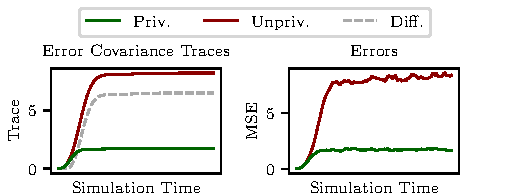
\includegraphics{figures/single_level_bounded.pdf}
    \caption{Privileged estimation with bounded error covariance.}
    \label{fig:priv_estimation:est_sim_bounded}
    % TODO Make larger and make the colours match. Also, add a grid
\end{figure}
As expected, it can be seen that the privileged estimator's error covariance trace is lower than the unprivileged estimator's and that the privileged estimator has a lower MSE. The difference in trace between the two estimators has also been plotted and equals the trace of the series \eqref{eq:priv_estimation:est_covariance_difference_series} due to the simulation initial error covariance $\mat{0}$.

The second simulation considers an unobservable system where only state velocity is measured and has an unbounded error covariance as $k \rightarrow \infty$. It is given by 
\begin{equation}\label{eq:priv_estimation:est_simulation_measurement_model_unbounded}
    \mat{z}_k=
    \begin{bmatrix}
        0 & 0 & 1 & 0\\
        0 & 0 & 0 & 1
    \end{bmatrix}
    \vec{x}_k + \vec{v}_k\,,
\end{equation}
and the same noise distribution and keystream covariance $\mat{S}$ as in the bounded case. Figure \ref{fig:priv_estimation:est_sim_unbounded} shows the average error covariance traces and MSE of estimation from $1000$ simulation runs with models \eqref{eq:priv_estimation:est_simulation_system_model} and \eqref{eq:priv_estimation:est_simulation_measurement_model_unbounded} and shows similar results.
\begin{figure}[htbp]
    \centering
    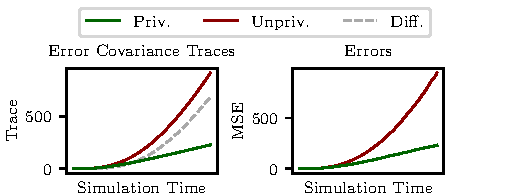
\includegraphics{figures/single_level_unbounded.pdf}
    \caption{Privileged estimation with unbounded error covariance.}
    \label{fig:priv_estimation:est_sim_unbounded}
    % TODO Make larger and make the colours match. Also, add a grid
\end{figure}

Both figures capture the difference in estimation error between the best possible estimators given the simulated processes (in terms of MSE) and support the security proof sketch in section \ref{subsec:priv_estimation:est_security}.

% 
% 8888888b.  8888888b.  8888888 888     888      8888888888 888     888  .d8888b.  8888888888 
% 888   Y88b 888   Y88b   888   888     888      888        888     888 d88P  Y88b 888        
% 888    888 888    888   888   888     888      888        888     888 Y88b.      888        
% 888   d88P 888   d88P   888   Y88b   d88P      8888888    888     888  "Y888b.   8888888    
% 8888888P"  8888888P"    888    Y88b d88P       888        888     888     "Y88b. 888        
% 888        888 T88b     888     Y88o88P        888        888     888       "888 888        
% 888        888  T88b    888      Y888P         888        Y88b. .d88P Y88b  d88P 888        
% 888        888   T88b 8888888     Y8P          888         "Y88888P"   "Y8888P"  8888888888 
%                                                                                             
%                                                                                             
%                                                                                             
% 

\section{Fusion in Privileged Estimation Environments}\label{sec:priv_estimation:privileged_fusion}
Recalling the problem formulation in section \ref{subsec:priv_estimation:fusion_problem}, an effective single-sensor privileged estimation scheme leads to interest in the extension to environments with multiple sensors, where multiple privileges and accesses to measurements are possible, affecting the estimation performance of present estimators. We aim to present a privileged fusion scheme where the Performance Loss Lower Bound (PLLB) and the Performance Gain Upper Bound (PGUB), defined in section \ref{subsec:priv_estimation:fusion_problem}, can be derived and proved using the covariance privilege notation in definition \ref{def:priv_estimation:covariance_privilege_notion}. The idea behind the scheme is to add \textit{correlated} Gaussian keystreams to the measurements from each sensor. These noises can be computed and subtracted by estimators holding respective sensor keys, while their correlation limits the additional information gained from fusing unprivileged measurements.

% 
%  ######   #######  ########  ########     ##    ## ######## ##    ##  ######  
% ##    ## ##     ## ##     ## ##     ##    ##   ##  ##        ##  ##  ##    ## 
% ##       ##     ## ##     ## ##     ##    ##  ##   ##         ####   ##       
% ##       ##     ## ########  ########     #####    ######      ##     ######  
% ##       ##     ## ##   ##   ##   ##      ##  ##   ##          ##          ## 
% ##    ## ##     ## ##    ##  ##    ##     ##   ##  ##          ##    ##    ## 
%  ######   #######  ##     ## ##     ##    ##    ## ########    ##     ######  
% 

\subsection{Correlated Gaussian Keystreams}\label{subsec:priv_estimation:fus_gaussian_keystreams}
Similarly to the multivariate Gaussian keystream in section \ref{subsec:priv_estimation:est_gaussian_keystream}, pseudorandom samples can be correlated in this way even when generated using different stream cipher keys. To parameterise the correlation between noises at each sensor, we introduce a fully correlated component $\mat{V}\in\mathbb{R}^{m\times m}$, $\mat{V}\succ\mat{0}$, and an uncorrelated component $\mat{W}\in\mathbb{R}^{m\times m}$, $\mat{W}\succ\mat{0}$, and define a noise cross-correlation matrix for $x$ noises as $\mat{S}^{(x)} \in \mathbb{R}^{xm\times xm}$,
\begin{equation}\label{eq:priv_estimation:fus_noise_correlation_matrix}
    \mat{S}^{(x)}=
    \begin{bmatrix}
        \mat{V} & \cdots & \mat{V}\\
        \vdots & \ddots & \vdots\\
        \mat{V} & \cdots & \mat{V}\\
    \end{bmatrix}+
    \begin{bmatrix}
        \mat{W} & \mat{0} & \mat{0}\\
        \mat{0} & \ddots & \mat{0}\\
        \mat{0} & \mat{0} & \mat{W}\\
    \end{bmatrix}\,,
\end{equation}
and $\mat{S}^{(1)}=\mat{V}+\mat{W}$. Denoting generated multivariate standard Gaussian noise \eqref{eq:priv_estimation:est_gaussian_standard_noise_stream} and added Gaussian noise \eqref{eq:priv_estimation:est_gaussian_noise_stream} for sensor $i$ at timestep $k$ as $\vec{\psi}_{k, i}$ and $\vec{g}_{k, i}$, respectively, the generation of all $n$ multivariate Gaussian noises at timestep $k$, $\vec{g}_k^{(1:n)}$, can be computed. This can be done by
\begin{equation}\label{eq:priv_estimation:fus_all_correlated_noises_generation}
    \vec{g}_k^{(1:n)}=
    \begin{bmatrix}
        \vec{g}_{k,1}\\
        \vdots\\
        \vec{g}_{k,n}
    \end{bmatrix}=
    \mat{S}^{(n)\frac{1}{2}}\cdot
    \begin{bmatrix}
        \vec{\psi}_{k,1}\\
        \vdots\\
        \vec{\psi}_{k,n}
    \end{bmatrix}\,,
\end{equation}
where each $\vec{\psi}_{k, i}$ is computed as $\vec{\psi}_k$ in \eqref{eq:priv_estimation:est_gaussian_standard_noise_stream} using uniform samples generated with key $\mathsf{sk}_{\mathsf{g}, i}$, and $\mat{S}^{(n)\frac{1}{2}}$ is a matrix such that $\mat{S}^{(n)\frac{1}{2}}\mat{S}^{(n)\frac{1}{2}\top}=\mat{S}^{(n)}$. Notably, as we consider sequential access to keys, it is important that the vector of the first $\pi$ noises $\vec{g}_{k, i}$, $1\leq i\leq \pi$, in \eqref{eq:priv_estimation:fus_all_correlated_noises_generation}, denoted $\vec{g}_k^{(1:\pi)}$, can be reproduced by an estimator of privilege $\pi$, holding only the keys $\mathsf{sk}_{\mathsf{g}, i}$, $1\leq i\leq \pi$. One case where this is possible is when a lower-triangular decomposition, such as the Cholesky decomposition, is used to compute $\mat{S}^{(n)\frac{1}{2}}$ from $\mat{S}^{(n)}$. Then, each correlated Gaussian sample $\vec{g}_{k,i}$ is computable from preceding standard samples $\vec{\psi}_{k,j}$, $j\leq i$ only, and the generalised noise generation equation
\begin{equation}\label{eq:priv_estimation:fus_p_correlated_noises_generation}
  \vec{g}_k^{(1:\pi)}=
  \mat{S}^{(\pi)\frac{1}{2}}\cdot
  \begin{bmatrix}
    \vec{\psi}_{k,1}\\
    \vdots\\
    \vec{\psi}_{k,\pi}
  \end{bmatrix}
\end{equation}
generates the same first $\pi$ noises $\vec{g}_k^{(1:\pi)}$ as would be obtained from \eqref{eq:priv_estimation:fus_all_correlated_noises_generation}. This is due to $\mat{S}^{(\pi)\frac{1}{2}}\in\mathbb{R}^{\pi m\times \pi m}$ equalling the top left block of matrix $\mat{S}^{(n)\frac{1}{2}}$ when using the lower-triangular decomposition.

At every timestep $k$, $\vec{g}_k^{(1:n)}$ can be generated with \eqref{eq:priv_estimation:fus_p_correlated_noises_generation} using all $n$ keys and used to modify sensor measurements, while the subset $\vec{g}_k^{(1:\pi)}$ can be generated by estimators of privilege $\pi$ using only the keys they hold.

% 
% ##     ##  #######  ########  
% ###   ### ##     ## ##     ## 
% #### #### ##     ## ##     ## 
% ## ### ## ##     ## ##     ## 
% ##     ## ##     ## ##     ## 
% ##     ## ##     ## ##     ## 
% ##     ##  #######  ########  
% 

\subsection{Measurement Modification}\label{subsec:priv_estimation:fus_measurement_mod}
With a way to generate noises for sensors and estimators, we can introduce the means of measurement modification and the observable measurement models for different estimators in the multiple-sensor environment. Measurement modification is performed by adding noises $\vec{g}_k^{(1:n)}$ to measurements from each sensor $i$ before making them public, resulting in modified measurement equations for each sensor,
\begin{equation}\label{eq:priv_estimation:fus_modified_measurements}
    \vec{z}_{k,i}^\prime = \vec{z}_{k,i} + \vec{g}_{k, i} = \mat{H}_{k,i}\vec{x}_k + \vec{v}_{k,i} + \vec{g}_{k,i}\,,
\end{equation}
with measurement noise $\vec{v}_{k,i}\sim\mathcal{N}(\vec{0},\mat{R}_{k,i})$ and the vector of all added pseudorandom noises $\vec{g}_k^{(1:n)}\ \dot{\sim}\ \mathcal{N}(\vec{0}, \mat{S}^{(n)})$. As we assume that sensors are synchronised in $k$, we can capture the correlation between these modified measurements exactly by considering the stacked measurement model for any estimator with access to $\tau$ measurements at timestep $k$, as
\begin{equation}\label{eq:priv_estimation:fus_measurement_equation}
    \vec{z}_k^{\prime(1:\tau)} = \vec{z}_k^{(1:\tau)} + \vec{g}_k^{(1:\tau)} = \mat{H}_k^{(1:\tau)}\vec{x}_k + \vec{v}_k^{(1:\tau)} + \vec{g}_k^{(1:\tau)}\,,
\end{equation}
with $\vec{v}_k^{(1:\tau)}\sim\mathcal{N}(\vec{0},\mat{R}_k^{(1:\tau)})$ and $\vec{g}_k^{(1:\tau)}\ \dot{\sim}\ \mathcal{N}(\vec{0},\mat{S}^{(\tau)})$, where
\begin{equation*}
  \vec{z}_k^{\prime(1:\tau)}=
  \begin{bmatrix}
    \vec{z}_{k,1}^\prime\\
    \vdots\\
    \vec{z}_{k,\tau}^\prime
  \end{bmatrix},\ 
  \vec{z}_k^{(1:\tau)}=
  \begin{bmatrix}
    \vec{z}_{k,1}\\
    \vdots\\
    \vec{z}_{k,\tau}
  \end{bmatrix},\ 
  \mat{H}_k^{(1:\tau)}=
  \begin{bmatrix}
    \mat{H}_{k,1}\\
    \vdots\\
    \mat{H}_{k,\tau}\\
  \end{bmatrix}\,,
\end{equation*}
\begin{equation*}
  \vec{v}_k^{(1:\tau)}=
  \begin{bmatrix}
    \vec{v}_{k,1}\\
    \vdots\\
    \vec{v}_{k,\tau}
  \end{bmatrix},\ 
  \mat{R}_k^{(1:\tau)}=
    \begin{bmatrix}
      \mat{R}_{k,1} & \mat{0} & \mat{0}\\
      \mat{0} & \ddots & \mat{0}\\
      \mat{0} & \mat{0} & \mat{R}_{k,\tau}
    \end{bmatrix}\,
\end{equation*}
and $\mat{S}^{(\tau)} \in \mathbb{R}^{\tau m\times \tau m}$ defined by \eqref{eq:priv_estimation:fus_noise_correlation_matrix}.

Since we are using a cryptographically sound stream cipher to generate the added Gaussian keystream, the pseudorandom samples are indistinguishable from truly random ones to estimators without appropriate keys, which leads us to three observable measurement models, \textit{i.e.}, the models that capture all the information available to an estimator exactly, for three types of mutually exhaustive estimators. Recalling the estimator notation introduced in section \ref{subsec:priv_estimation:fusion_problem}, we have
\begin{description}
    \item[Estimators of the form $\mathsf{e}^{[0,\tau]}$] Here, no keys are held by an unprivileged estimator with access to $\tau$ measurements, thus all generated noises $\vec{g}_k^{(1:\tau)}$ are indistinguishable from noises from the truly random distribution $\mathcal{N}(\vec{0}, \mat{S}^{(\tau)})$. For these estimators, we can rewrite the measurement equation \eqref{eq:priv_estimation:fus_measurement_equation} as the observed measurement model
    \begin{equation}\label{eq:priv_estimation:fus_0q_obs_measurement_model}
        \vec{z}_k^{[0,\tau]} = \mat{H}_k^{(1:\tau)}\vec{x}_k + \vec{v}_k^{\prime}\,,
    \end{equation}
    with truly Gaussian term $\vec{v}_k^{\prime} \sim \mathcal{N}(\vec{0}, \mat{R}_k^{(1:\tau)}+\mat{S}^{(\tau)})$.
  
    \item[Estimators of the form $\mathsf{e}^{[\pi,\pi]}$] Estimators with keys for all the sensors to which they have access can generate all added noises and subtract them from the received measurements. That is, $\vec{g}_k^{(1:\pi)}$ can be generated and $\vec{z}_k^{[\pi,\pi]}=\vec{z}_k^{\prime(1:\pi)}-\vec{g}_k^{(1:\pi)}$ computed to give the observed measurement model equal to receiving unmodified measurements only,
    \begin{equation}\label{eq:priv_estimation:fus_pp_obs_measurement_model}
        \vec{z}_k^{[\pi,\pi]} = \mat{H}_k^{(1:\pi)}\vec{x}_k + \vec{v}_k^{(1:\pi)}\,,
    \end{equation}
    where $\vec{v}_k^{(1:\pi)} \sim \mathcal{N}(\vec{0}, \mat{R}_k^{(1:\pi)})$.

    \item[Estimators of the form $\mathsf{e}^{[\pi,\tau]}$, $\pi<\tau$] Lastly, we want the observed measurement model when only some accessible measurements can have their noises removed. Here, the noises from sensors $i>\pi$ which cannot be removed are conditionally dependent on the known noises $\vec{g}_k^{(1:\pi)}$. Since we can generate the noises $\vec{g}_k^{(1:\pi)}$ and know that $\vec{g}_k^{(1:\tau)}\ \dot{\sim}\ \mathcal{N}(\vec{0}, \mat{S}^{(\tau)})$, we can write 
    \begin{equation}\label{eq:priv_estimation:fus_block_noises_and_correlation}
        \vec{g}_k^{(1:\tau)}=
        \begin{bmatrix}
            \vec{g}_k^{(1:\pi)}\\
            \vec{g}_k^{(\pi+1:\tau)}\\
        \end{bmatrix}
        \ \dot{\sim}\ \mathcal{N}\left(
        \begin{bmatrix}
            \vec{0}\\
            \vec{0}
        \end{bmatrix},
        \begin{bmatrix}
            \mat{S}^{(\pi)} & \bar{\mat{V}}\\
            \bar{\mat{V}}^\top & \mat{S}^{(\tau-\pi)}
        \end{bmatrix}\right)\,,
    \end{equation}
    where $\bar{\mat{V}} \in \mathbb{R}^{\pi m \times (\tau-\pi)m}$ is a block matrix with every block equal to $\mat{V}$, and compute the conditional pseudorandom Gaussian distribution
    \begin{equation}\label{eq:priv_estimation:fus_conditional_noise_distribution}
        \vec{g}_k^{(\pi+1:\tau)} \mid \vec{g}_k^{(1:\pi)}
        \ \dot{\sim}\ \mathcal{N}\left(\bar{\mat{V}}^\top\mat{S}^{(\pi)-1}\vec{g}_k^{(1:\pi)},
        \mat{S}^{(\tau-\pi)} - \bar{\mat{V}}^\top\mat{S}^{(\pi)-1}\bar{\mat{V}}\right)\,.
    \end{equation}
    Now, subtracting the known noises $\vec{g}_k^{(1:\pi)}$ and the means of the unknown noises \eqref{eq:priv_estimation:fus_conditional_noise_distribution} from received measurements,
    \begin{equation}\label{eq:priv_estimation:fus_pq_measurement_offset}
        \vec{z}_k^{[\pi,\tau]}=\vec{z}_k^{\prime(1:\tau)} - 
        \begin{bmatrix}
        \vec{g}_k^{(1:\pi)}\\
        \bar{\mat{V}}^\top\mat{S}^{(\pi)-1}\vec{g}_k^{(1:\pi)}
        \end{bmatrix}\,,
    \end{equation}
    and accounting for unknown pseudorandom noises being indistinguishable from random, a zero-mean observed measurement model can be written as
    \begin{equation}\label{eq:priv_estimation:fus_pq_obs_measurement_model}
        \vec{z}_k^{[\pi,\tau]} = \mat{H}_k^{(1:\tau)}\vec{x}_k + \vec{v}_k^{\prime}
    \end{equation}
    where 
    \begin{equation}
        \vec{v}_k^{\prime} \sim \mathcal{N}\left(\vec{0},
        \begin{bmatrix}
            \mat{R}_k^{(1:\pi)} & \mat{0}\\
            \mat{0} & \mat{S}^{(\tau-\pi)} - \bar{\mat{V}}^\top\mat{S}^{(\pi)-1}\bar{\mat{V}} + \mat{R}_k^{(\pi+1:\tau)}
        \end{bmatrix}\right).
    \end{equation}
\end{description}
\begin{remark}
    Recalling that we assume estimators access unprivileged measurements sequentially to simplify notation, \eqref{eq:priv_estimation:fus_block_noises_and_correlation}, \eqref{eq:priv_estimation:fus_pq_measurement_offset} and \eqref{eq:priv_estimation:fus_pq_obs_measurement_model} can be generalised when having access to arbitrary $\tau-\pi$ non-sequential unprivileged measurements $\vec{z}_{k, i}$, $\pi <i\leq \tau$, by appropriately rearranging the columns of $\mat{S}^{(\tau-\pi)}$ in \eqref{eq:priv_estimation:fus_block_noises_and_correlation}.
\end{remark}

From the observed measurement models \eqref{eq:priv_estimation:fus_0q_obs_measurement_model}, \eqref{eq:priv_estimation:fus_pp_obs_measurement_model} and \eqref{eq:priv_estimation:fus_pq_obs_measurement_model} we can tell that the parameters $\mat{V}$ and $\mat{W}$ (within matrices $\mat{S}^{(\tau)}$, $\mat{S}^{(\pi)}$ and $\mat{S}^{(\tau-\pi)}$) will control the difference in estimation performance between the three types of estimators. Computing the two bounds we wish to cryptographically guarantee, PLLB and PGUB, respectively, and how $\mat{V}$ and $\mat{W}$ affect them, will be more formally explored in sections \ref{subsec:priv_estimation:fus_security} and \ref{subsec:priv_estimation:fus_simulation}.

% 
% ##    ##  #######  ####  ######  ########    ########  ####  ######  ######## 
% ###   ## ##     ##  ##  ##    ## ##          ##     ##  ##  ##    ##    ##    
% ####  ## ##     ##  ##  ##       ##          ##     ##  ##  ##          ##    
% ## ## ## ##     ##  ##   ######  ######      ##     ##  ##   ######     ##    
% ##  #### ##     ##  ##        ## ##          ##     ##  ##        ##    ##    
% ##   ### ##     ##  ##  ##    ## ##          ##     ##  ##  ##    ##    ##    
% ##    ##  #######  ####  ######  ########    ########  ####  ######     ##    
% 

\subsection{Distribution of Noise Terms}\label{subsec:priv_estimation:fus_noise_dist}
While we have described a method for generating noises that modify $n$ measurements and result in different observed measurement models depending on estimator privilege, we have not discussed where the noise is generated and how it is distributed to sensors. To handle the inherent correlation of the noises $\vec{g}_{k}^{(1:n)}$, here we briefly consider how they can be generated either centrally before distribution to sensors or sequentially at the sensors themselves, given previously generated values.
\begin{description}
    \item[Central noise generation] To compute noises centrally, \eqref{eq:priv_estimation:fus_p_correlated_noises_generation} can be computed for all $n$ noises at a central processor and each noise $\vec{g}_{k,i}$ sent to the respective sensor $i$ before it modifies its local measurement by \eqref{eq:priv_estimation:fus_modified_measurements}.
    \item[Sequential noise generation] To compute the same noises sequentially for each timestep $k$, sensor $1$ can generate its noise independently using its current standard Gaussian sample $\vec{z}_{k,1}$, by $\vec{g}_{k,1} = \mat{S}^{(1)\frac{1}{2}}\vec{\psi}_{k,1}$. Each following sensor $i>1$ can generate its noise $\vec{g}_{k,i}$ given the preceding noises $\vec{g}_k^{(1:i-1)}$ and following the conditional reasoning in \eqref{eq:priv_estimation:fus_conditional_noise_distribution}, as
    \begin{equation}
        \vec{g}_{k,i} = \bar{\mat{V}}^\top\mat{S}^{(i-1)-1}\vec{g}_k^{(1:i-1)} +
        (\mat{S}^{(1)}-\bar{\mat{V}}^\top\mat{S}^{(i-1)-1}\bar{\mat{V}})^\frac{1}{2}\vec{\psi}_{k,i}\,.
    \end{equation}
    After local noise generation, sensor $i$ sends its and preceding noises, $\vec{g}_k^{(1:i)}$, to the next sensor $i+1$. This method has the clear downside of increasing communication costs with each successive generation but requires no central communicator.
\end{description}
In both cases above, the computation of all noises $\vec{g}_k^{(1:n)}$ can be performed offline, reducing the complexity of real-time measurement modification.

% 
%  ######  ########  ##    ## ########  ########  #######  
% ##    ## ##     ##  ##  ##  ##     ##    ##    ##     ## 
% ##       ##     ##   ####   ##     ##    ##    ##     ## 
% ##       ########     ##    ########     ##    ##     ## 
% ##       ##   ##      ##    ##           ##    ##     ## 
% ##    ## ##    ##     ##    ##           ##    ##     ## 
%  ######  ##     ##    ##    ##           ##     #######  
% 
\subsection{Security Analysis}\label{subsec:priv_estimation:fus_security}
The security analysis of the fusion problem aims to give proof sketches of the desired estimation performance differences. As in the single-sensor case, we again assume floating-point numbers to be sufficiently close to real random numbers such that the optimality of the linear KF in section \ref{subsec:prelims:kf_opt} holds, and recall that all sensors are synchronised in timestep $k$, leading to observed measurement models \eqref{eq:priv_estimation:fus_0q_obs_measurement_model}, \eqref{eq:priv_estimation:fus_pp_obs_measurement_model} and \eqref{eq:priv_estimation:fus_pq_obs_measurement_model} being exactly correct. Similarly to the proof sketch in section \ref{subsec:priv_estimation:est_security}, these assumptions are used to produce a series of covariances for optimal estimators before taking their difference to obtain the semi-definite series corresponding to the PLLB and PGUB. The series can then be used as the sequence $\mat{D}_1,\mat{D}_2,\dots$ in definition \ref{def:priv_estimation:covariance_privilege_notion} for individual proofs of appropriate privilege estimation schemes for the two bounds. As before, the existence of an estimator violating the notion implies the existence of a linear estimator with error covariance lower than the KF, proving the bounds by contrapositive.

% 
% .##........#######...######...######.....########...#######..##.....##.##....##.########.
% .##.......##.....##.##....##.##....##....##.....##.##.....##.##.....##.###...##.##.....##
% .##.......##.....##.##.......##..........##.....##.##.....##.##.....##.####..##.##.....##
% .##.......##.....##..######...######.....########..##.....##.##.....##.##.##.##.##.....##
% .##.......##.....##.......##.......##....##.....##.##.....##.##.....##.##..####.##.....##
% .##.......##.....##.##....##.##....##....##.....##.##.....##.##.....##.##...###.##.....##
% .########..#######...######...######.....########...#######...#######..##....##.########.
% 

\subsubsection{Performance Loss Lower Bound (PLLB)}
First, we consider the lower bound to the loss in estimation performance an estimator $\mathsf{e}^{[0,N]}$ has on an estimator $\mathsf{e}^{[p,p]}$ when measurements follow the presented scheme. Since the observed measurement models for these estimators, \eqref{eqn:0q_obs_measurement_model} and \eqref{eqn:pp_obs_measurement_model}, interpret available measurements as a single stacked measurement, and since we do not consider estimators that corrupt sensors, we can treat the stacked measurement as coming from a single sensor and use the notion of covariance privilege in definition [def:cov\_priv\_security\_notion] to guarantee the bound. The associated privileged estimation scheme for the PLLB can be written for each privilege $p$ as
\begin{description}
  \item[$\mathsf{Setup}$] Given the system model [eqn:system\_model], all measurements models [eqn:measurement\_models] (interpretable as a single stacked measurement model) and a security parameter $\kappa$ used by all sensors, generate $N$ stream cipher keys $\mathsf{sk_i}$, $1\leq i \leq N$, and let the secret key $\mathsf{sk}$ include all $N$ keys. Generate the correlated and uncorrelated noise components $\mat{Z}$ and $\mat{Y}$, an initial estimate and error covariance $\hat{\vec{x}}_0$ and $\mat{P}_0$, and include these in the public parameters $\mathsf{pub}$.
  
  \item[$\mathsf{Noise}_{\mathsf{PLLB}}$] Given parameters, cipher keys, a timestep $k$ and true sensor measurements $\vec{y}_k^{(1:N)}$, let $\vec{y}_k^{\{\mathsf{up}\}}=\vec{y}_k^{[0,N]}$ following \eqref{eqn:0q_obs_measurement_model} and $\vec{y}_k^{\{\mathsf{p}\}}=\vec{y}_k^{[p,p]}$ following \eqref{eqn:pp_obs_measurement_model}.
\end{description}
With the above formulation, we can use the KF to recursively compute the optimal estimate error covariances for estimators with access to only measurements $\vec{y}_k^{\{\mathsf{up}\}}$ or $\vec{y}_k^{\{\mathsf{p}\}}$, for all $k$. Since the KF preserves initial covariance order, $\mat{P}_k \succeq \mat{P}_k^\prime \implies \mat{P}_{k+1} \succeq \mat{P}_{k+1}^\prime$, a lower bound can be guaranteed when using the initial covariance $\mat{P}_0=\mat{0}$. Therefore, the minimum achievable error covariance for an estimator $\mathsf{e}^{[0,N]}$, with access to measurements $\vec{y}_k^{\{\mathsf{up}\}}=\vec{y}_k^{[0,N]}$, is given by the combined KF predict and update equations
\begin{equation}\label{eqn:0N_lower_bound_covariance}
  \begin{split}
    \mat{P}_k^{[0,N]} =& \Bigl( \mat{I} - (\mat{F}_k\mat{P}_{k-1}^{[0,N]}\mat{F}_k^\top + \mat{Q}_k)\mat{H}_k^{(1:N)\top} \cdot \\
    &\quad\bigl(\mat{H}_k^{(1:N)}(\mat{F}_k\mat{P}_{k-1}^{[0,N]}\mat{F}_k^\top + \mat{Q}_k)\mat{H}_k^{(1:N)\top} \\
    &\quad+ \mat{R}_k^{(1:N)} + \mat{S}^{(N)}\bigr)^{-1}\mat{H}_k^{(1:N)}\Bigr)\cdot\\
    &\Bigl(\mat{F}_k\mat{P}_{k-1}^{[0,N]}\mat{F}_k^\top + \mat{Q}_k\Bigr)\,,
 \end{split}
\end{equation}
when $\mat{P}_0^{[0,N]}=\mat{0}$. Similarly, the same can be done for an estimator $\mathsf{e}^{[p,p]}$, with access to measurements $\vec{y}_k^{\{\mathsf{p}\}}=\vec{y}_k^{[p,p]}$, as
\begin{equation}\label{eqn:pp_lower_bound_covariance}
  \begin{split}
    \mat{P}_k^{[p,p]} =& \Bigl( \mat{I} - (\mat{F}_k\mat{P}_{k-1}^{[p,p]}\mat{F}_k^\top + \mat{Q}_k)\mat{H}_k^{(1:p)\top} \cdot \\
    &\quad\bigl(\mat{H}_k^{(1:p)}(\mat{F}_k\mat{P}_{k-1}^{[p,p]}\mat{F}_k^\top + \mat{Q}_k)\mat{H}_k^{(1:p)\top} \\
    &\quad+ \mat{R}_k^{(1:p)}\bigr)^{-1}\mat{H}_k^{(1:p)}\Bigr)\cdot\\
    &\Bigl(\mat{F}_k\mat{P}_{k-1}^{[p,p]}\mat{F}_k^\top + \mat{Q}_k\Bigr)
  \end{split}
\end{equation}
and $\mat{P}_0^{[p,p]}=\mat{0}$. The bounds \eqref{eqn:0N_lower_bound_covariance} and \eqref{eqn:pp_lower_bound_covariance} are constructed such that at every timestep $k$,
\begin{equation}\label{eqn:0N_cov_bound}
  \begin{split}
    &\mat{P}_k^{[0,N]} \preceq\\
    &\qquad \mathsf{Cov}\left[\mathcal{A}\left(k,\mathcal{M}_S,\mathcal{M}_M,\vec{y}_1^{[0,N]},\dots,\vec{y}_k^{[0,N]}\right) - \vec{x}_k\right]
  \end{split}
\end{equation}
and
\begin{equation}\label{eqn:pp_cov_bound}
  \begin{split}
    &\mat{P}_k^{[p,p]} \preceq\\
    &\qquad \mathsf{Cov}\left[\mathcal{A}\left(k,\mathcal{M}_S,\mathcal{M}_M,\vec{y}_1^{[p,p]},\dots,\vec{y}_k^{[p,p]}\right) - \vec{x}_k\right]
  \end{split}
\end{equation}
hold. Recalling definition [def:cov\_priv\_security\_notion], and knowing that the minimum achievable covariance of the estimators is produced using the KF, it can be seen that the difference 
\begin{equation}\label{eqn:unpriv_priv_pllb_difference_series}
  \mat{D}_{\mathsf{PLLB},k} = \mat{P}_k^{[0,N]} - \mat{P}_k^{[p,p]}\,
\end{equation}
produces a series where for any PPT estimator $\mathsf{e}^{[0,N]}$, an equivalent PPT estimator $\mathsf{e}^{[p,p]}$, lower bounded in error by \eqref{eqn:pp_lower_bound_covariance}, can always be created such that the difference between their error covariances at time $k$ is at least $\mat{D}_{\mathsf{PLLB},k}$. Here, the PPT requirement guarantees the indistinguishabilty of pseudorandom streams to truly random ones and a negligible performance gain for $\mathsf{e}^{[0,N]}$ is present on average if secret keys or keystreams are guessed. The existence of an estimator of the form $\mathsf{e}^{[0,N]}$ where this condition cannot be met, implies the existence of an estimator with error covariances smaller than the KF for linear models. As no such estimator exists, we conclude that the $\mathsf{Setup}$ and $\mathsf{Noise_{\mathsf{PLLB}}}$ algorithms above meet \textit{$\{\mat{D}_{\mathsf{PLLB},1},\mat{D}_{\mathsf{PLLB},2},\dots\}$-Covariance Privilege for System Model [eqn:system\_model] and Stacked Measurement Models [eqn:measurement\_models]}.

In the above, we lower bound the estimation performance loss an estimator $\mathsf{e}^{[0,N]}$ has on estimators $\mathsf{e}^{[p,p]}$. In the cases where the unprivileged estimator has access to fewer measurements, $\mathsf{e}^{[0,q]}$, $q<N$, or the privileged one to more, $\mathsf{e}^{[p,q]}$, $q>p$, the achievable difference can only increase (fewer measurements can only increase error covariance while more can only decrease it). This ensures the computed bound remains a lower bound for \textit{any} unprivileged estimator.

% 
% ..######......###....####.##....##....########...#######..##.....##.##....##.########.
% .##....##....##.##....##..###...##....##.....##.##.....##.##.....##.###...##.##.....##
% .##.........##...##...##..####..##....##.....##.##.....##.##.....##.####..##.##.....##
% .##...####.##.....##..##..##.##.##....########..##.....##.##.....##.##.##.##.##.....##
% .##....##..#########..##..##..####....##.....##.##.....##.##.....##.##..####.##.....##
% .##....##..##.....##..##..##...###....##.....##.##.....##.##.....##.##...###.##.....##
% ..######...##.....##.####.##....##....########...#######...#######..##....##.########.
% 

\subsubsection{Performance Gain Upper Bound (PGUB)}
Similar to the lower bound above, we can use the same properties of the KF to give an upper bound to the gain in estimation performance an estimator $\mathsf{e}^{[p,N]}$ has on an estimator $\mathsf{e}^{[p,p]}$ when measurements follow the presented scheme. The associated privileged estimation scheme for the PGUB for each privilege $p$ is given by the same $\mathsf{Setup}$ algorithm as in section [subsec:crypto\_performance\_loss\_lower\_bound] and
\begin{description}
  \item[$\mathsf{Noise}_{\mathsf{PGUB}}$] Given parameters, cipher keys, a timestep $k$ and true sensor measurements $\vec{y}_k^{(1:N)}$, let $\vec{y}_k^{\{\mathsf{up}\}}=\vec{y}_k^{[p,N]}$ following \eqref{eqn:pq_obs_measurement_model} and $\vec{y}_k^{\{\mathsf{p}\}}=\vec{y}_k^{[p,p]}$ following \eqref{eqn:pp_obs_measurement_model}.
\end{description}
The minimum error covariances achievable by an estimator $\mathsf{e}^{[p,p]}$ is again given by \eqref{eqn:pp_lower_bound_covariance} and $\mat{P}_0^{[p,p]} = \mat{0}$. For an estimator $\mathsf{e}^{[p,N]}$ with access to measurements $\vec{y}_k^{\{\mathsf{up}\}}=\vec{y}_k^{[p,N]}$ it is given by
\begin{equation}\label{eqn:pN_lower_bound_covariance}
  \begin{split}
    \mat{P}_k^{[p,N]} =& \Bigl( \mat{I} - (\mat{F}_k\mat{P}_{k-1}^{[p,N]}\mat{F}_k^\top + \mat{Q}_k)\mat{H}_k^{(1:N)\top} \cdot \\
    &\quad\bigl(\mat{H}_k^{(1:N)}(\mat{F}_k\mat{P}_{k-1}^{[p,N]}\mat{F}_k^\top + \mat{Q}_k)\mat{H}_k^{(1:N)\top} \\
    &\quad+ \mat{X}\bigr)^{-1}\mat{H}_k^{(1:N)}\Bigr)\Bigl(\mat{F}_k\mat{P}_{k-1}^{[p,N]}\mat{F}_k^\top + \mat{Q}_k\Bigr)\,,
 \end{split}
\end{equation}
where
\begin{equation}
  \mat{X} = 
  \begin{bmatrix}
    \mat{R}_k^{(1:p)} & \mat{0}\\
    \mat{0} & \mat{S}^{(N-p)} - \bar{\mat{Z}}^\top\mat{S}^{(p)-1}\bar{\mat{Z}} + \mat{R}_k^{(p+1:N)}
  \end{bmatrix}
\end{equation}
and $\mat{P}_0^{[p,N]} = \mat{0}$. Again, the bounding series are such that \eqref{eqn:pp_cov_bound} and
\begin{equation}\label{eqn:pN_cov_bound}
  \begin{split}
    &\mat{P}_k^{[p,N]} \preceq\\
    &\qquad \mathsf{Cov}\left[\mathcal{A}\left(k,\mathcal{M}_S,\mathcal{M}_M,\vec{y}_1^{[p,N]},\dots,\vec{y}_k^{[p,N]}\right) - \vec{x}_k\right]
  \end{split}
\end{equation}
hold. Now, the difference
\begin{equation}\label{eqn:unpriv_priv_pgub_difference_series}
  \mat{D}_{\mathsf{PGUB},k} = \mat{P}_k^{[p,N]} - \mat{P}_k^{[p,p]}\,
\end{equation}
produces a series where for any PPT estimator $\mathsf{e}^{[p,N]}$, an equivalent PPT estimator $\mathsf{e}^{[p,p]}$, lower bounded in error by \eqref{eqn:pp_lower_bound_covariance}, can always be created such that the difference between their error covariances at time $k$ is at least $\mat{D}_{\mathsf{PGUB},k}$. With the same reasoning as for the lower bound, we conclude that the $\mathsf{Setup}$ and $\mathsf{Noise}_{\mathsf{PGUB}}$ algorithms above meet \textit{$\{\mat{D}_{\mathsf{PGUB},1},\mat{D}_{\mathsf{PGUB},2},\dots\}$-Covariance Privilege for System Model [eqn:system\_model] and Stacked Measurement Models [eqn:measurement\_models]}.

In \eqref{eqn:unpriv_priv_pgub_difference_series}, $\mat{D}_{\mathsf{PGUB},k} \preceq 0$ for all $k>0$ and lower bounds the (negative) loss in performance an estimator $\mathsf{e}^{[p,N]}$ has on estimators $\mathsf{e}^{[p,p]}$. We refer to the bound as an upper bound as its negation $-\mat{D}_{\mathsf{PGUB},k}$, $k>0$, upper bounds the estimation performance gain achievable by $\mathsf{e}^{[p,N]}$ on the estimators $\mathsf{e}^{[p,p]}$, as desired in section [sec:prob]. In the case where fewer unprivileged measurements are accessible, $\mathsf{e}^{[p,q]}$, $q<N$, this gain can only decrease, keeping the upper bound valid for any estimators $\mathsf{e}^{[p,q]}$, $q>p$.

% 
% .##....##..#######..##....##.........##.......####.##....##
% .###...##.##.....##.###...##.........##........##..###...##
% .####..##.##.....##.####..##.........##........##..####..##
% .##.##.##.##.....##.##.##.##.#######.##........##..##.##.##
% .##..####.##.....##.##..####.........##........##..##..####
% .##...###.##.....##.##...###.........##........##..##...###
% .##....##..#######..##....##.........########.####.##....##
% 

\subsubsection{Non-Linear Systems}

% 
%  ######  #### ##     ## 
% ##    ##  ##  ###   ### 
% ##        ##  #### #### 
%  ######   ##  ## ### ## 
%       ##  ##  ##     ## 
% ##    ##  ##  ##     ## 
%  ######  #### ##     ## 
% 
\subsection{Simulation}\label{subsec:priv_estimation:fus_simulation}
In addition to showing how the estimation performance loss and gain bounds can be computed, we have simulated optimal estimators to demonstrate the effects of the correlated and uncorrelated components, $\mat{Z}$ and $\mat{Y}$, respectively. The state of an aircraft $\begin{bmatrix}x & y & v_x & v_y\end{bmatrix}^\top$, capturing its position $x$, $y$ (m) and velocity $v_x$, $v_y$ (m/s), was simulated following a constant velocity system model given by [eqn:system\_model] with parameters
\begin{equation}
  \mat{F}_k=
  \begin{bmatrix}
     1 & 0.5 & 0 & 0\\
     0 & 1 & 0 & 0\\
     0 & 0 & 1 & 0.5\\
     0 & 0 & 0 & 1
  \end{bmatrix}\,,
\end{equation}
and
\begin{equation}
  \mat{Q}_k=10^{-3}\cdot
  \begin{bmatrix}
     0.42 & 1.25 & 0 & 0\\
     1.25 & 5 & 0 & 0\\
     0 & 0 & 0.42 & 1.25\\
     0 & 0 & 1.25 & 5
  \end{bmatrix}\,,
\end{equation}
for all $k$, and measured independently by location sensors $i$, $1\leq i \leq N=4$, following [eqn:measurement\_models] with constant parameters
\begin{equation}
  \mat{H}_{k,i}=
  \begin{bmatrix}
     1 & 0 & 0 & 0\\
     0 & 0 & 1 & 0
  \end{bmatrix}
  \text{ and }
  \mat{R}_{k,i}=
  \begin{bmatrix}
     5 & 2\\
     2 & 5
  \end{bmatrix}\,,
\end{equation}
for all $k$. Simulations were implemented in the Python programming language and the considered correlated and uncorrelated parameters were restricted to the forms $\mat{Z}=\Sigma_z\cdot\mat{I}$ and $\mat{Y}=\Sigma_y\cdot\mat{I}$ for simplicity. All estimators executed linear Kalman filters with the parameters above and the exact knowledge of the initial state ($\mat{P}_0=\mat{0}$).

Figure \ref{fig:mse_privs} shows the errors of different privileged estimators with access to varying sensor measurements when added noise parameters $\Sigma_z$ and $\Sigma_y$ are held constant. As would be expected, the error decreases when more keys are available, while a further decrease is achieved as more additional unprivileged measurements are fused. Here, the difference in mean squared error (MSE) between $\mathsf{e}^{[0,4]}$ and $\mathsf{e}^{[p,p]}$ (shaded blue region), and between $\mathsf{e}^{[p,p]}$ and $\mathsf{e}^{[p,4]}$ (shaded red region), are bounded on average by the trace of the PLLB series \eqref{eqn:unpriv_priv_pllb_difference_series} and PGUB series \eqref{eqn:unpriv_priv_pgub_difference_series}, respectively, when $\Sigma_z=2$ and $\Sigma_y=10$.
\begin{figure}[htbp]
  \centering
  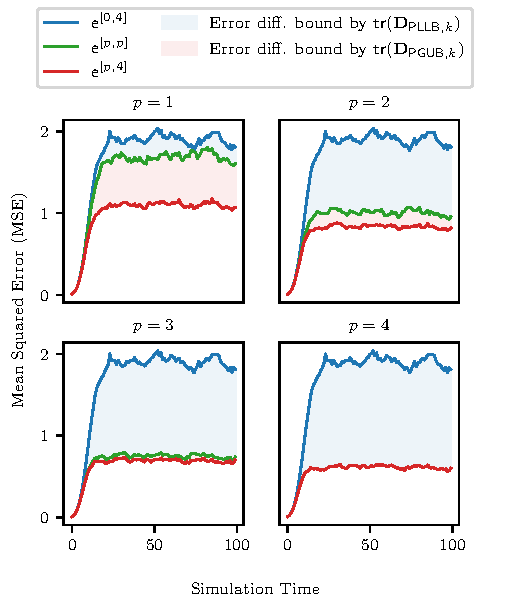
\includegraphics{figures/mse_privs.pdf}
  \caption{The average errors of different estimators for $1000$ simulation runs when $\Sigma_z=2$ and $\Sigma_y=10$.}
  \label{fig:mse_privs}
\end{figure}

To demonstrate the effect of parameters $\Sigma_z$ and $\Sigma_y$ (and therefore $\mat{Z}$ and $\mat{Y}$), figure \ref{fig:mse_params} shows their effect on the MSE given fixed estimators. It can be seen that $\Sigma_z$ has a more prominent effect on the PLLB while $\Sigma_y$ has it on the PGUB. However, it can also be observed that both parameters affect both bounds to some degree, revealing some limitations when specific bounds are desired using the proposed scheme.
\begin{figure}[htbp]
  \centering
  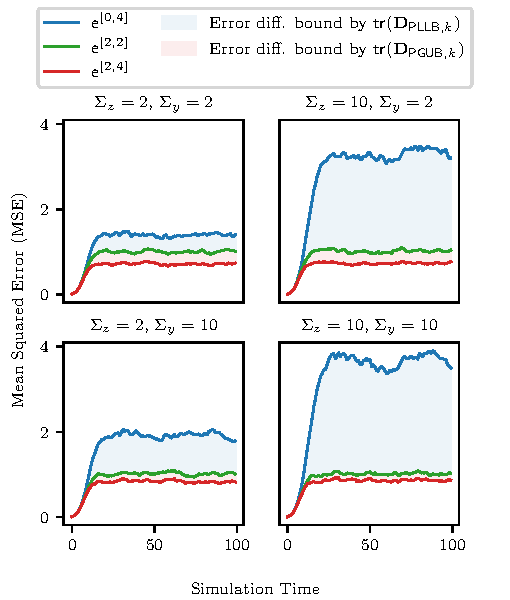
\includegraphics{figures/mse_params.pdf}
  \caption{The average errors of unprivileged and privilege-$2$ estimators for $1000$ simulation runs when varying $\Sigma_z$ and $\Sigma_y$.}
  \label{fig:mse_params}
\end{figure}
Figure \ref{fig:trace_params} further captures this relation between the bounds and the parameters $\Sigma_z$ and $\Sigma_y$. As the simulated system is asymptotically stable, steady-state error covariances are reached as $k \to \infty$, and therefore $\mat{D}_{\mathsf{PLLB},k}$ and $\mat{D}_{\mathsf{PGUB},k}$ stabilise as well. From the plot, we can see that increasing the fully correlated noise parameter $\Sigma_z$ cannot greatly reduce the PGUB (\textit{i.e.}, bring $\mathsf{tr}(\mat{D}_{\mathsf{PGUB},k})$ closer to $0$), likely due to the accurate estimation of this component by privileged estimators and the remaining uncorrelated component staying unchanged. Simultaneously, however, the fully correlated component can greatly increase the PLLB (\textit{i.e.}, take $\mathsf{tr}(\mat{D}_{\mathsf{PLLB},k})$ further from $0$) as it increases the redundancy of fusing only unprivileged measurements. The effects of increasing $\Sigma_y$ are less one-sided. The PGUB is reduced due to sufficient uncorrelated noise making the fusion of unprivileged measurements hold little information even when some keys are known, but the PLLB is increased, as uncorrelated noise still affects estimators fusing only unprivileged measurements, albeit less drastically.

Figure \ref{fig:trace_params} also shows how the bounds are affected by the privilege $p$ they are computed for. Predictably, a higher privilege results in fewer additional unprivileged measurements to fuse, lowering the PGUB, but also producing better privileged estimates, increasing the PLLB. We can also see that when the fully correlated noise term $\Sigma_z$ is small and privilege is low ($p=1$), unprivileged estimators with access to all measurements can perform better than privileged ones accessing only privileged measurements (resulting in a negative $\mathsf{tr}(\mat{D}_{\mathsf{PLLB},k})$).
\begin{figure}[htbp]
  \centering
  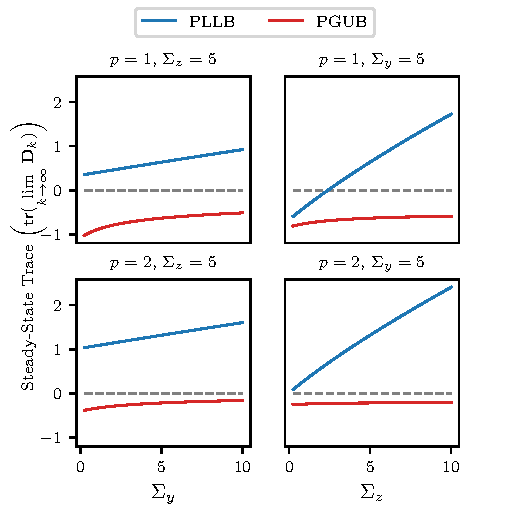
\includegraphics{figures/trace_params.pdf}
  \caption{Steady-state traces of the PLLB and PGUB for privileges $p=1$ and $p=2$ when $\Sigma_z$ and $\Sigma_y$ are varied.}
  \label{fig:trace_params}
\end{figure}

% 
%  .d8888b.   .d88888b.  888b    888  .d8888b.  
% d88P  Y88b d88P" "Y88b 8888b   888 d88P  Y88b 
% 888    888 888     888 88888b  888 888    888 
% 888        888     888 888Y88b 888 888        
% 888        888     888 888 Y88b888 888        
% 888    888 888     888 888  Y88888 888    888 
% Y88b  d88P Y88b. .d88P 888   Y8888 Y88b  d88P 
%  "Y8888P"   "Y88888P"  888    Y888  "Y8888P"  
%                                               
%                                               
%                                               
% 

\section{Conclusions on Provable Estimation Performances}\label{sec:priv_estimation:conclusion}
% In this work, we have presented the idea of a privileged estimation scheme and given a formal cryptographic definition for its security. A concrete scheme was provided that meets this notion and an intuitive extension to multiple privilege levels was discussed. A simulation demonstrating a simple use case has been presented, while the benefits of controlling estimation accuracy on a per-party basis have wide application from privatized localization hardware to subscription-based data access. Future work on the topic includes achieving formal security for broader model requirements and testing our scheme on dedicated hardware to demonstrate the method's real-time capability. 



% The presented method demonstrates how different levels of estimation performance can be cryptographically guaranteed in a network of multiple sensors. The problem considered requires sequential access to sensors and sensor keys and allows for two free parameters, $\mat{Z}$ and $\mat{Y}$, to loosely control the two relevant cryptographic bounds. The different bounds for each privilege, changing bounds over time and the relation between these parameters and the bounds themselves mean that choosing these parameters is a task-specific problem where care must be taken to meet any desired bounds without overly affecting others. The resulting cryptographic bounds can, however, always be computed exactly.

% Future work on this topic includes deriving parameters that affect the relevant cryptographic bounds independently, relaxing sequential sensor and key access requirements and exploring methods for decentralised correlated noise generation with fewer communication costs.

\chapter{Conclusion}\label{ch:conclusion}


Led to the publication of several works in peer-reviewed journals, journal letters and conferences [].

% 
%        d8888 8888888b.  8888888b.  8888888888 888b    888 8888888b. 8888888 Y88b   d88P 
%       d88888 888   Y88b 888   Y88b 888        8888b   888 888  "Y88b  888    Y88b d88P  
%      d88P888 888    888 888    888 888        88888b  888 888    888  888     Y88o88P   
%     d88P 888 888   d88P 888   d88P 8888888    888Y88b 888 888    888  888      Y888P    
%    d88P  888 8888888P"  8888888P"  888        888 Y88b888 888    888  888      d888b    
%   d88P   888 888        888        888        888  Y88888 888    888  888     d88888b   
%  d8888888888 888        888        888        888   Y8888 888  .d88P  888    d88P Y88b  
% d88P     888 888        888        8888888888 888    Y888 8888888P" 8888888 d88P   Y88b 
%                                                                                         
%                                                                                         
%                                                                                         
% 
\appendix

\chapter{Linear-Combination Aggregator Obliviousness}\label{app:lcao_definition}
The following game between attacker and challenger defines the security notion of LCAO.
\begin{description}
    \item[Setup] The challenger chooses security parameter $\kappa$, runs the $\mathsf{Setup}(\kappa)$ algorithm and gives $\mathsf{pub}$, $m$ and $pk_0$ to the attacker
    \item[Queries] The attacker can now perform encryptions or submit queries that are answered by the challenger. The types of actions are:
    \begin{enumerate}
        \item \textit{Encryption:} The attacker chooses a value $x$ and computes an encryption of $x$ under the aggregator's public key $pk_0$, obtaining $\mathcal{E}_{pk_0}(x)$.
        \item \textit{Weight Queries:} The attacker chooses an instance $t$ and receives the weights for that instance encrypted with the aggregator's public key, $\mathcal{E}_{pk_0}(\omega^{(t)}_{j}),\,j\in\{1,\dots,m\}$.
        \item \textit{Combine Queries:} The attacker chooses a tuple $(i,t,a^{(t)}_{i,1},\dots,a^{(t)}_{i,m})$ such that for any two chosen combine query tuples $(i,t,a^{(t)}_{i,1},\dots,a^{(t)}_{i,m})$ and $(i',t',a^{\prime(t')}_{i',1},\dots,a^{\prime(t')}_{i',m})$, the following condition holds:
        \begin{equation*}
            i = i' \wedge t = t' \implies a^{(t)}_{i,j} = a^{\prime(t')}_{i',j},\,j\in\{1,\dots,m\}\,.
        \end{equation*}
        The attacker is then given back the encryption of the linear combination $\mathcal{E}_{pk_0,sk_i}(\sum^m_{j=1}a^{(t)}_{i,j}\omega^{(t)}_j)$ encrypted under both the aggregator public key $pk_0$ and the secret key $sk_i$.
        \item \textit{Compromise queries:} The attacker chooses $i$ and receives the secret key $sk_i$. The aggregator's secret key may also be compromised (when choosing $i=0$).
    \end{enumerate} 
    \item[Challenge] Next, the attacker chooses an instance $t^*$, and a subset of users $S \subseteq U$ where $U$ is the complete set of users for which no combine queries, for the instance $t^*$, and no compromise queries, are made for the duration of the game. The attacker then chooses two series of tuples
    \begin{equation*}
        \left\langle\left(i,t^*,a^{(t^*)(0)}_{i,1},\dots,a^{(t^*)(0)}_{i,m}\right)\,\middle|\,i \in S\right\rangle
    \end{equation*}
    and
    \begin{equation*}
        \left\langle\left(i,t^*,a^{(t^*)(1)}_{i,1},\dots,a^{(t^*)(1)}_{i,m}\right)\,\middle|\, i \in S\right\rangle\,,
    \end{equation*}
    and gives them to the challenger. In the case that $0 \in S$ (\textit{i.e.}, the aggregator is compromised) and $S = U$, it is additionally required that
    \begin{equation*}
        \sum_{i\in S}\sum^{m}_{j=1} a^{(t^*)(0)}_{i,j}\omega^{(t^*)}_j = \sum_{i \in S}\sum^{m}_{j=1} a^{(t^*)(1)}_{i,j}\omega^{(t^*)}_j\,,
    \end{equation*}
    for weights $\omega^{(t^*)}_j,\,j\in\{1,\dots,m\}$ returned by a \textit{Weight Query} with chosen instance $t^*$. The challenger then chooses a random bit $b \in \{1,0\}$ and returns encryptions 
    \begin{equation*}
        \left\langle\mathcal{E}_{pk_0,sk_i}\left(\sum^m_{j=1}a^{(t^*)(b)}_{i,j}\omega^{(t^*)}_j\right)\,\middle|\,i\in S\right\rangle\,.
    \end{equation*}
    \item[More Queries] The attacker can now perform more encryptions and submit queries, so long as the queries do not break the requirements in the Challenge stage. That is, $S \subseteq U$.
    \item[Guess] At the end, the attacker outputs a bit $b'$ and wins the game if and only if $b' = b$. The advantage of an attacker $\mathcal{A}$ is defined as
    \begin{equation*}
        \mathsf{Adv}^{LCAO}(\mathcal{A}) \coloneqq \left\lvert \Pr [b'=b] - \frac{1}{2}\right\rvert\,.
    \end{equation*} 
\end{description}

\begin{definition}
    An encryption scheme meets LCAO security if no probabilistic adversary, running in polynomial-time with respect to security parameter $\kappa$, has more than a negligible advantage in winning the above security game. That is, for all adversaries $\mathcal{A}$, there exists a negligible function $\eta$, such that
    \begin{equation*}
        \mathsf{Adv}^{LCAO}(\mathcal{A}) \leq \eta(\kappa)\,,
    \end{equation*}
    with probabilities taken over randomness introduced by $\mathcal{A}$, and in $\mathsf{Setup}$, $\mathsf{Enc}$ and $\mathsf{CombEnc}$.
\end{definition}

\chapter{Cryptographic Proof of LCAO Scheme Security}

% 
% 8888888b.  8888888888 8888888888 .d8888b.  
% 888   Y88b 888        888       d88P  Y88b 
% 888    888 888        888       Y88b.      
% 888   d88P 8888888    8888888    "Y888b.   
% 8888888P"  888        888           "Y88b. 
% 888 T88b   888        888             "888 
% 888  T88b  888        888       Y88b  d88P 
% 888   T88b 8888888888 888        "Y8888P"  
%                                            
%                                            
%                                            
% 
\backmatter
% List of algorithms
\listoffigures
\listoftables
% Bibliography
\bibliographystyle{IEEEtran}
\bibliography{bibliography/dissertation-marko-ristic}
% Index

\end{document}